\documentclass[lang=cn,10pt]{elegantbook}

\title{Project 02: 多重网格(Multigrid)}

\author{Wenchong Huang}
\date{April 10, 2023}

\setcounter{tocdepth}{3}

\logo{logo-blue.jpg}
\cover{cover.jpeg}
\usepackage{multirow}
\usepackage{xpatch}
\makeatletter
\xpatchcmd{\chapter}
  {\if@openright\cleardoublepage\else\clearpage\fi}{\par\relax}
  {}{}
\makeatother

% 本文档命令
\usepackage{array, float}
\newcommand{\ccr}[1]{\makecell{{\color{#1}\rule{1cm}{1cm}}}}

% 修改标题页的橙色带
% \definecolor{customcolor}{RGB}{32,178,170}
% \colorlet{coverlinecolor}{customcolor}

\begin{document}

\maketitle
\frontmatter

\tableofcontents

\mainmatter

\chapter{用户手册}

\section{编译与测试说明}

若想编译并运行本文的所有测试(不包含第六章),请在项目根目录下执行:
\begin{lstlisting}
  make run
\end{lstlisting}

初次编译需要编译jsoncpp,大约需要一分钟。

本文有一些极限测试,这些测试使用的网格极大,因此会占用您大量的系统内存,请保证至少4G的可用内存。完整运行测试需要大约20分钟。

若想清除编译过程产生的所有文件,请在项目根目录下执行:
\begin{lstlisting}
  make clean
\end{lstlisting}

\section{方程与参数的自定义说明}

您需要将方程按下列格式描述,并保存为json文件。下面是样例1:
\begin{lstlisting}
  {
    "Condition Type": "Dirichlet",
    "Dimension": 1,
    "Grid Size": 4194304,
    "f": "(sin(x)-cos(x)*cos(x))*exp(sin(x))",
    "g": {
        "x=0": "1",
        "x=1": "exp(sin(1))"
    },
    "Cycle Type": "FMG",
    "Max Iter": 5,
    "eps": 1e-16,
    "Restriction": "full operator",
    "Prolongation": "quadradic",
    "Error Check": true,
    "u": "exp(sin(x))"
  }
\end{lstlisting}

下面是样例2:
\begin{lstlisting}
  {
    "Condition Type": "mixed",
    "Dimension": 2,
    "Reigeon Type": "Irregular",
    "Grid Size": 64,
    "f": "-(1-sin(x)+cos(x)*cos(x))*exp(sin(x)+y)",
    "g": {
        "x=0": ["-cos(x)*exp(sin(x)+y)", "Neumann"],
        "x=1": ["exp(sin(x)+y)", "Dirichlet"],
        "Down Bondary": ["cos(x)*exp(sin(x)+y)*(pi/16*cos(pi*x))/sqrt(pi*pi/256*(cos(pi*x))^2+1)+exp(sin(x)+y)*(-1)/sqrt(pi*pi/256*(cos(pi*x))^2+1)", "Neumann"],
        "y=1": ["exp(sin(x)+y)", "Neumann"]
    },
    "Cycle Type": "FMG",
    "Restriction": "full operator",
    "Prolongation": "linear",
    "Max Iter": 3,
    "eps": 1e-6,
    "Error Check": true,
    "u": "exp(sin(x)+y)"
}
\end{lstlisting}

各参数说明如下:

\begin{enumerate}[(1)]
\item \verb|Condition Type|是条件的类型,您可以输入\verb|Dirichlet|,\verb|Neumann|或\verb|mixed|;
\item \verb|Dimension|是维数,您可以输入1或2
\item \verb|Reigeon Type|是区域的类型,您可以输入\verb|Regular|或\verb|Irregular|;
\item \verb|Grid Size|是网格的大小,您需要输入一个正整数,并且必须为2的正整数次幂;
\item \verb|Center|与\verb|Radius|用于描述不规则区域的形状;
\item \verb|f|用于描述$-\Delta u$;
\item \verb|g|用于描述边值条件,请按不同边界列出,按样例1所示。如果您的条件类型是\verb|mixed|,您必须按照样例2的写法列出边界条件。
\item \verb|Cycle Type|:Cycle的类型。您可以输入\verb|V|或\verb|FMG|。
\item \verb|Restriction|:限制算子的类型。您可以输入\verb|injection|或\verb|full operator|。
\item \verb|Prolongation|:插值算子的类型。您可以输入\verb|linear|或\verb|quadradic|。
\item \verb|Max Iter|:最大迭代次数。您可以输入一个正整数。
\item \verb|eps|:求解精度需求。您可以输入一个正浮点数。
\item \verb|Check Error|:若您需要验证误差,请设为\verb|true|,否则设为\verb|false|;
\item \verb|u|:真实解。如果您需要验证误差,您必须提供真实解的表达式。
\end{enumerate}

使用
\begin{lstlisting}
    ./solve 文件名
\end{lstlisting}

来求解您的方程。

\newpage

\chapter{设计手册}

\section{求解器类与继承关系}

在这个Project中,我们放弃了10分的模板类附加分,并不是因为不会写,而是我们认为有更加优美的设计方式。事实上,模板类的缺点很明显,您只能将源代码写在\verb|.h|头文件中,这会让您的头文件显得杂乱不堪,您无法像我们一样在头文件中只声明类与函数,在源程序中实现函数。另外,如果您使用了\verb|template<int dim>|,那么您的代码一定四处充斥着诸如\verb|if(dim==1)...else...|的判断,这是丑陋的。现在请让我们向您提供一种更加优美的设计方式。

首先,定义根求解器,如下:
\begin{lstlisting}
  class rootSolver{
    protected:
        int n; // Grid Size
        ColVector cur, b;
        const Operator & restriction;
        const Operator & prolongation;
        std::string bondary;
        BType bonDetail;
        double eps;
        int maxiter;
        int dim;
        std::vector<SparseMatrix> Ah;
        int cycle; // cycle=1:V-Cycle  cycle=2:FMG-Cycle
        bool pure_Neumann;
        double neumannC;
        bool irregular;
        virtual SparseMatrix getAh(const int &n) const = 0;
        void initAh();
        ColVector VC(const int &d, const int &n, ColVector v, const ColVector &f);
        ColVector FMG(const int &d, const int &n, const ColVector &f);
    
    public:
        rootSolver(const Operator & restriction, const Operator & prolongation);
        void init(const int &_n, const Function &f, const Function &g, const std::string &bon);
        virtual void init(const int &_n, const Function &f, const Function &g, const std::string &bon, const BType &bonDetail) = 0;
        void setEps(const double &_eps);
        void setMaxiter(const int &N);
        void setCycle(const std::string &cy);
        void setIrregular(const bool &rhs);
        void solve();
        bool isPureNeumann() const;
        virtual void output(std::ostream& fout) const = 0;
        virtual double calcNeumannC(const Function &u) = 0;
        virtual double checkError(const Function &u, const Norm &norm) const = 0;
    };
\end{lstlisting}

这是一个不能直接实例化的类。事实上,成员变量与大部分成员函数对于一维和二维而言都是一样的,因此我们将其声明在根求解器中,并实现它们。对于一维和二维情况下不一样的函数,我们在根求解器中将其声明为虚函数,由子类实现。下面定义一维与二维求解器:
\begin{lstlisting}
  class Solver1D : public rootSolver{
    private:
        SparseMatrix getAh(const int &n) const;
    public:
        Solver1D(const Operator & restriction, const Operator & prolongation);
        void init(const int &_n, const Function &f, const Function &g, const std::string &bon, const BType &bonDetail);
        void output(std::ostream& fout) const;
        double calcNeumannC(const Function &u);
        double checkError(const Function &u, const Norm &norm) const;
    };
    
    class Solver2D : public rootSolver{
    private:
        SparseMatrix getAh(const int &n) const;
    public:
        Solver2D(const Operator & restriction, const Operator & prolongation);
        void init(const int &_n, const Function &f, const Function &g, const std::string &bon, const BType &bonDetail);
        void output(std::ostream& fout) const;
        double calcNeumannC(const Function &u);
        double checkError(const Function &u, const Norm &norm) const;
    };
\end{lstlisting}

它们继承了根求解器,并将根求解器中的虚函数实化。

\section{算子类与继承关系}

所有的算子都是算子基类的子类。算子基类定义如下:
\begin{lstlisting}
  class Operator{
    protected:
        int dim;
        bool irregular;
    public:
        Operator(const int &_dim);
        virtual ColVector operator () (const ColVector &v) const = 0;
        void setIrregular(const bool &rhs);
    };
\end{lstlisting}

一个算子需要继承算子基类,并定义\verb|()|运算,例如\verb|injection|算子定义如下:
\begin{lstlisting}
  class injection : public Operator{
  public:
      injection(const int &_dim);
      ColVector operator () (const ColVector &v) const;
  };
\end{lstlisting}

\section{表达式解析器}

为了让用户能够自定义方程而不必重新编译,我们设计了一个表达式解析器\verb|mathExpr|,内部实现使用了简单的堆栈与递归,能够支持所有的基本运算与初等函数。声明略。

用户只需将表达式以字符串格式传入,并将变量定义好,再添加一些自定义的常量,就可以求表达式的值。下面是一个例子,计算$u(x,y)=e^{\sin x+y}+C\;(C=2)$在$x=y=0.5$处的点值。
\begin{lstlisting}
  Expression expr;                    // 定义解析器
  expr.setExpr("exp(sin(x)+y)+C");    // 传入表达式
  expr.addConstant("C", 2);           // 声明常量
  expr.addVariable("x");              // 声明变量
  expr.addVariable("y");
  vector<double> parm(2);             // 以vector格式传入各变量值
  parm[0] = parm[1] = 0.5;
  cout << expr(parm) << endl;
\end{lstlisting}

\section{面向用户的二次封装}

考虑到求解器的设计比较复杂,对于用户并不友好,我们进行了二次封装。二次封装实现了一个类\verb|BVP|,声明如下。
\begin{lstlisting}
  class BVP{
  private:
      Json::Value problem;
      rootSolver *solver;

  public:
      BVP();
      BVP(const Json::Value & prob);
      BVP(const char * ifile);
      BVP(const std::string & ifile);

      void checkParse();
      void printProblem();
      void read(const char * ifile);
      void read(const std::string & ifile);
      void read(const Json::Value & prob);
      void solve();
      void output(std::ostream & out);
      void output(const std::string & ofile);
      void output();
      std::vector<double> checkError();
  };
\end{lstlisting}

用户只需写一个json(格式见1.2节)作为输入,既可以用\verb|.json|文件,也可以直接传入一个\verb|Json::Value|对象。这里以文件输入为例,给出用户通过二次封装来调用求解器的示例。
\begin{lstlisting}
  BVP bvp;
  bvp.read("input.json");                 // 读取输入文件input.json
  bvp.printProblem();                     // 将问题的基本信息输出
  bvp.solve();                            // 求解问题
  bvp.output("result.txt");               // 将解输出到文件result.txt中
  vector<double>err = bvp.checkError();   // 检查1范数、2范数、无穷范数下的误差
\end{lstlisting}

\section{迭代的设计要点与优化}

\subsection{正常终止与被迫终止}

正常终止有两种情况:达到给定最大迭代次数,或达到预设求解精度。后者的判断如下。

假设第$i$次迭代的结果为$\mathbf{v}$,第$i+1$次迭代的结果为$\mathbf{v}+\mathbf{v}'$,当$\mathbf{v}'<\text{eps}$时,终止迭代,以$\mathbf{v}+\mathbf{v}'$作为最终结果。

有时候,在用户指定的网格大小下,由于离散误差的存在,无法达到用户的预设精度,此时离散方程组的求解已经达到最佳,再迭代下去毫无意义,因此被迫中止。判断条件如下。

假设第$i$次迭代的结果为$\mathbf{v}$,第$i+1$次迭代的结果为$\mathbf{v}+\mathbf{v}'$,第$i+2$次迭代的结果为$\mathbf{v}+\mathbf{v}'+\mathbf{v}''$,当$||\mathbf{v}''||_\infty>||\mathbf{v}'||_\infty$时,终止迭代,以$\mathbf{v}+\mathbf{v}'$作为最终结果。

\subsection{FMG-Cycle的重复迭代}

很多同学认为,FMG-Cycle没有初始值的输入,因此只能执行一次迭代,所以求解精度不如多次迭代的V-Cycle。这是完全错误的。事实上,假设FMG-Cycle第一次迭代的结果为$\mathbf{v}$,我们可以令$\mathbf{f}'=\mathbf{f}-A\mathbf{v}$,然后将$\mathbf{f'}$作为方程右边提供给求解器,重复FMG-Cycle求得$\mathbf{v}'$,此时$\mathbf{v}+\mathbf{v}'$即为两次FMG-Cycle的结果。如此反复,就可以让FMG-Cycle执行多次迭代,以达到更高的求解精度。

事实上,将V-Cycle的迭代方式也改成这样,比每次传入$\mathbf{v}$重复迭代,效果要更好。因此我们的设计中统一采用了这种迭代方式。

\subsection{$A^h$的预算优化}

在一些naive的设计中,往往是在每一层V-Cycle的开始计算出这一层的$A^h$,然后在这一层返回后,计算出的$A^h$就被销毁。这样会存在大量的内存申请与释放。众所周知,现代计算设备的瓶颈在于内存,而不是CPU,因此上述过程对计算资源的浪费极大。

我们提出的方案是在求解器solve过程的开始,预先算出每一层V-Cycle需要用到的$A^h$,用一个数组存储。接下来每次迭代,每一层V-Cycle,直接以常量引用的方式使用预先算好的$A^h$即可,不存在内存的重复申请与复制。在整个求解过程结束后,再销毁所有的$A^h$。

实验证明,这样的处理方式能将程序提速2至3倍。

\subsection{纯Neumann条件下矩阵不适定的处理方法}

我们不对方程做任何形式的扰动,直接使用多重网格求解。事实上,尽管Jacobi迭代是发散的,但是存在一个一维的解空间,在迭代的过程中,当前解与解空间的距离会越来越小,因此我们总是能收敛到一个解。

我们得到的解与真实解相差一个常数$C$,在检查真实误差时,我们取真实解减去数值解的最大最小值平均,作为$C$的值,然后将数值解加上$C$后进行误差估计。

\newpage

\chapter{一维区域中的BVP}

\section{设计要点}

\subsection{一维区域的二次插值}

考虑用$ih,(i+1)h,(i+2)h$处的点值插值得到$ih+\frac{h}{2}$处的点值。事实上,三点唯一确定一个二次函数,直接待定系数法求出函数,再将$ih+\frac{h}{2}$代入即可,公式为:
\begin{equation}
  U^{h/2}_{2i+1} = \frac{3}{8}U^h_{i} + \frac{6}{8}U^h_{i+1} - \frac{1}{8}U^h_{i+2} + O(h^3).
\end{equation}

这样得到的公式关于$x=ih+\frac{h}{2}$不对称,为了使插值系数更加对称,我们用$(i-1)h,ih,(i+1)h$处的点值再做一次二次插值,得到:
\begin{equation}
  U^{h/2}_{2i+1} = \frac{6}{8}U^h_{i} + \frac{3}{8}U^h_{i+1} - \frac{1}{8}U^h_{i-1} + O(h^3).
\end{equation}

将上面两式相加,再乘$\frac{1}{2}$,即可得到中心对称的二次插值公式:
\begin{equation}
  U^{h/2}_{2i+1} = \frac{9}{16}U^h_{i} + \frac{9}{16}U^h_{i+1} - \frac{1}{16}U^h_{i-1} - \frac{1}{16}U^h_{i+2} + O(h^3).
\end{equation}

对于靠近边界的点,直接使用公式(3.3)会有访问越界风险,需要视点的位置使用不那么对称的(3.1)或(3.2)。

\section{数值实验}

\subsection{Dirichlet边值问题的求解、误差分析、收敛性分析}

考虑由精确解$u(x)=e^{\sin x}$导出的Dirichlet边值问题
\begin{equation}
  \left\{
    \begin{array}{l}
      -u''(x) = (\sin x-\cos^2 x)e^{\sin x},\quad x\in\Omega \\
      u(0)=0,\quad u(1)=e^{\sin 1}
    \end{array}
  \right. .
\end{equation}

我们用$n=512,1024,...,32768$的网格测试,使用FMG-Cycle,限制算子选择Full Operator,插值算子选择二次插值。当$n=512,...,4096$时,误差分布如下图所示。

\begin{figure}[H]
  \centering
  \begin{minipage}[t]{0.24\linewidth}
      \centering
      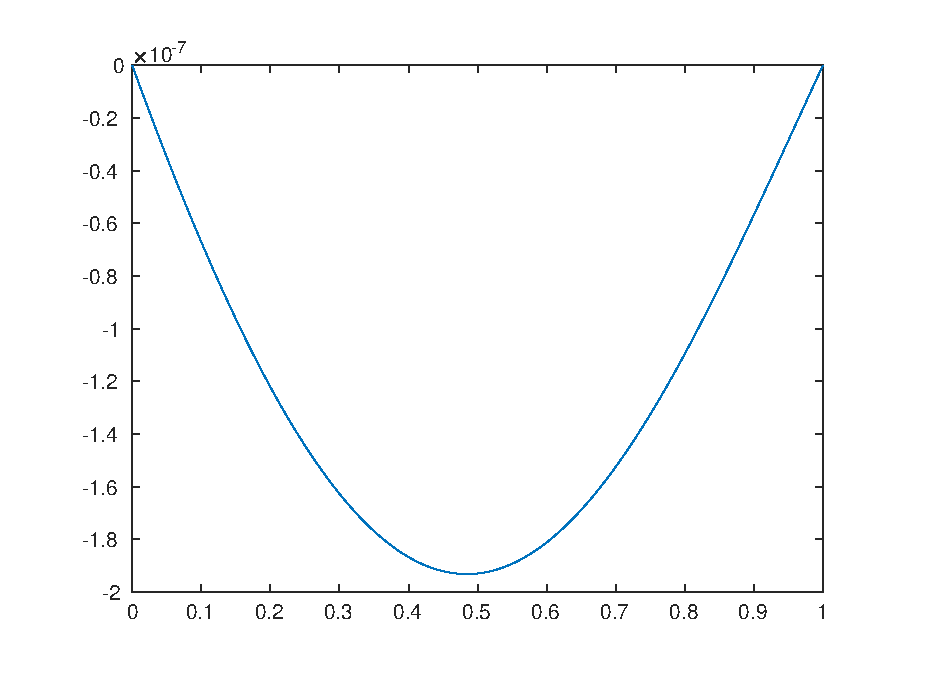
\includegraphics[width=0.95\linewidth]{figure/1-1-1.eps}
      \caption*{$n=512$}
  \end{minipage}
  \begin{minipage}[t]{0.24\linewidth}
    \centering
    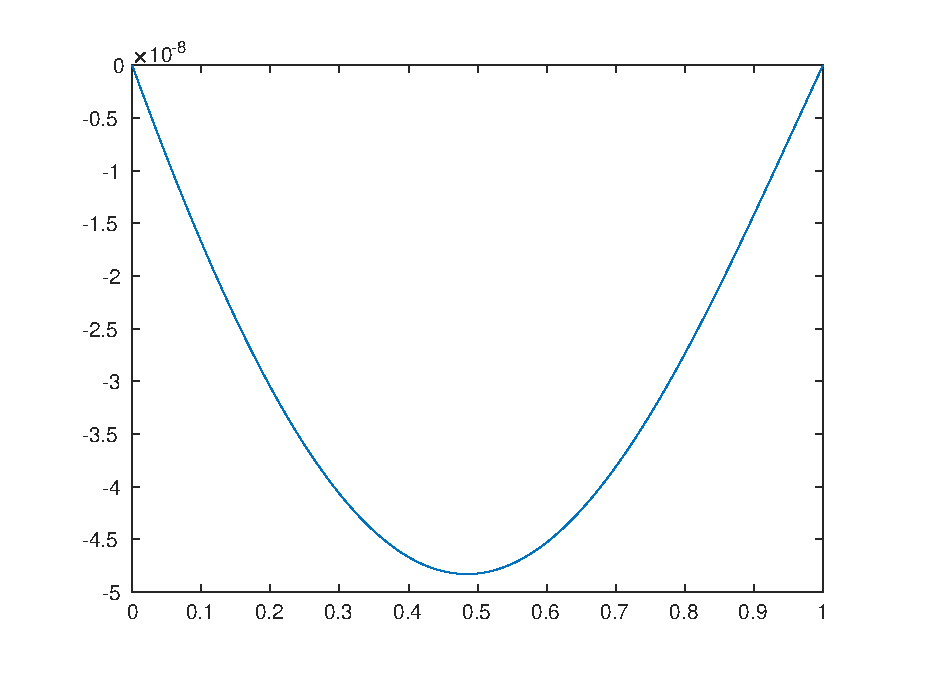
\includegraphics[width=0.95\linewidth]{figure/1-1-2.eps}
    \caption*{$n=1024$}
  \end{minipage}
  \begin{minipage}[t]{0.24\linewidth}
    \centering
    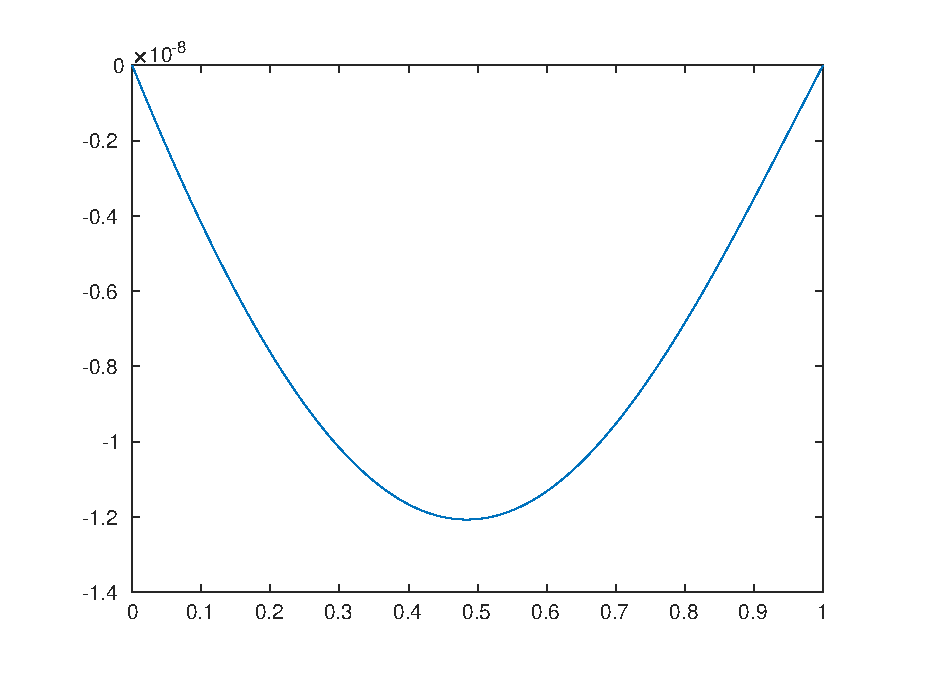
\includegraphics[width=0.95\linewidth]{figure/1-1-3.eps}
    \caption*{$n=2048$}
  \end{minipage}
  \begin{minipage}[t]{0.24\linewidth}
    \centering
    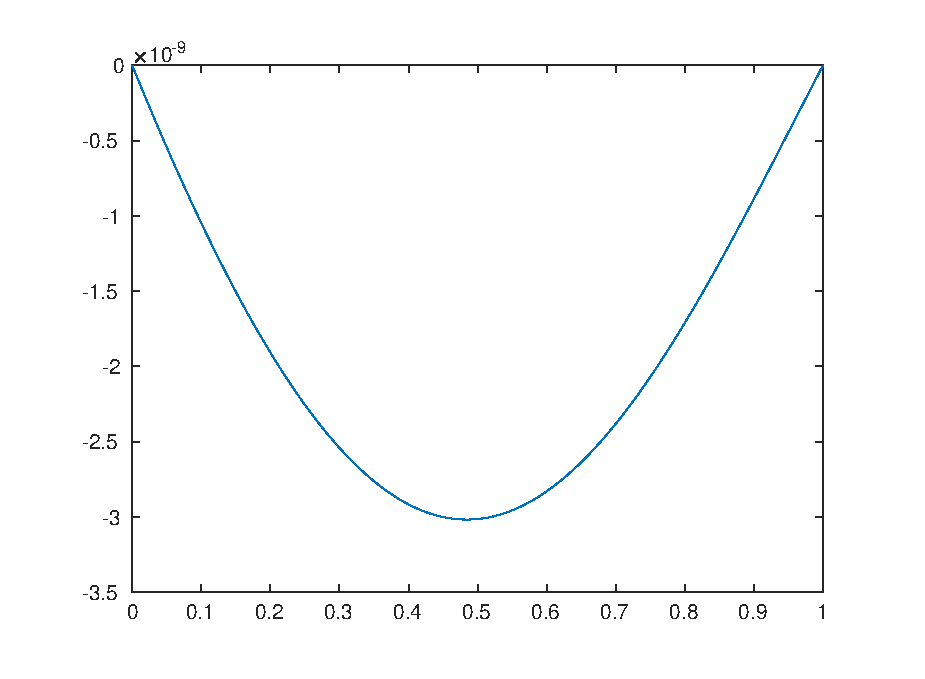
\includegraphics[width=0.95\linewidth]{figure/1-1-4.eps}
    \caption*{$n=4096$}
  \end{minipage}
\end{figure}

可以看到,在Dirichlet条件下,格点越靠近边界,最终的计算误差越小。将数值解与真实解的误差用范数估计,并根据$n=16384$增加到$n=32768$时误差减小的倍数,估计各范数下的收敛阶,结果如下表。

\begin{table}[H]
  \centering
  \small
  \begin{tabular}{c|ccccccc|c}
  \textbf{$n$}        & 512                 & 1024                 & 2048                 & 4096                 & 8192                 & 16384                & 32768                & 收敛阶 \\ \hline
  $||\cdot||_1$      & $1.24\times 10^{-7}$ & $3.10\times 10^{-8}$ & $7.76\times 10^{-9}$ & $1.94\times 10^{-9}$ & $4.85\times 10^{-10}$ & $1.21\times 10^{-10}$ & $3.03\times 10^{-11}$ & $2.000$\\
  $||\cdot||_2$      & $1.37\times 10^{-7}$ & $3.44\times 10^{-8}$ & $8.60\times 10^{-9}$ & $2.15\times 10^{-9}$ & $5.37\times 10^{-10}$ & $1.34\times 10^{-10}$ & $3.36\times 10^{-11}$ & $2.000$\\
  $||\cdot||_\infty$ & $1.93\times 10^{-7}$ & $4.83\times 10^{-8}$ & $1.21\times 10^{-8}$ & $3.02\times 10^{-9}$ & $7.54\times 10^{-10}$ & $1.89\times 10^{-10}$ & $4.72\times 10^{-11}$ & $2.000$
  \end{tabular}
\end{table}

符合二阶收敛的理论结果。

\subsection{Neumann边值问题的求解、误差分析、收敛性分析}

考虑由精确解$u(x)=e^{\sin x}$导出的Neumann边值问题
\begin{equation}
  \left\{
    \begin{array}{l}
      -u''(x) = (\sin x-\cos^2 x)e^{\sin x},\quad x\in\Omega \\
      u'(0)=1,\quad u'(1)=\cos 1\cdot e^{\sin 1}
    \end{array}
  \right. .
\end{equation}

我们用$n=512,1024,...,32768$的网格测试,使用FMG-Cycle,限制算子选择Full Operator,插值算子选择二次插值。当$n=512,...,4096$时,误差分布如下图所示。

\begin{figure}[H]
  \centering
  \begin{minipage}[t]{0.24\linewidth}
      \centering
      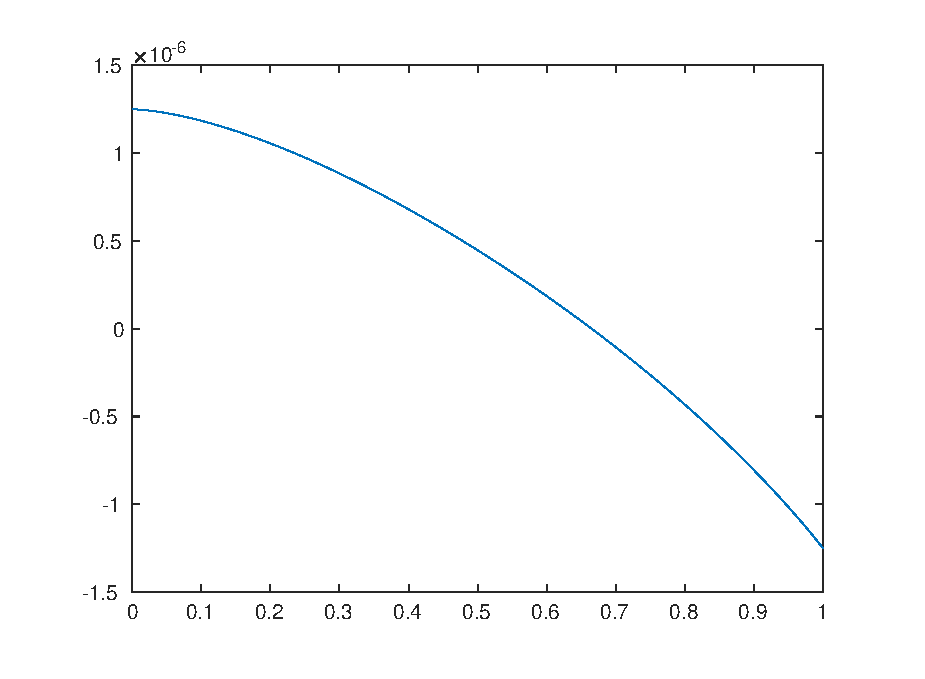
\includegraphics[width=0.8\linewidth]{figure/1-2-1.eps}
      \caption*{$n=512$}
  \end{minipage}
  \begin{minipage}[t]{0.24\linewidth}
    \centering
    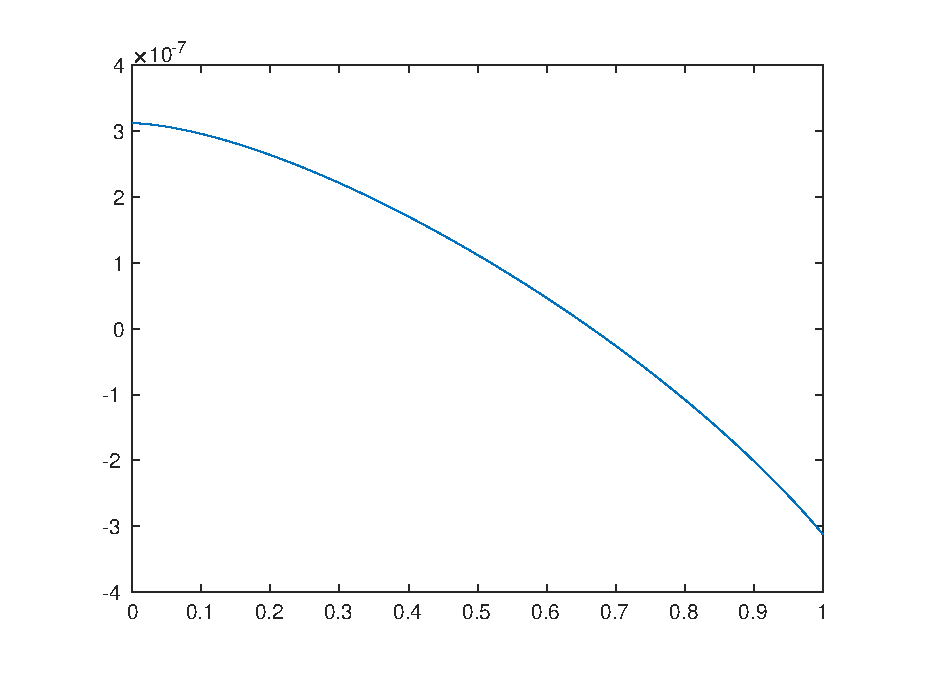
\includegraphics[width=0.8\linewidth]{figure/1-2-2.eps}
    \caption*{$n=1024$}
  \end{minipage}
  \begin{minipage}[t]{0.24\linewidth}
    \centering
    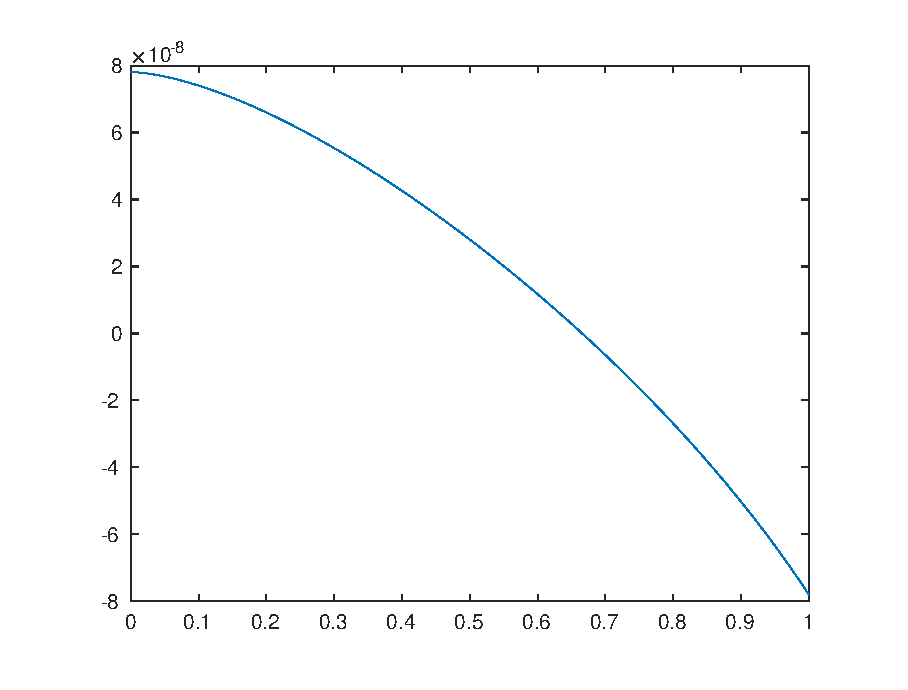
\includegraphics[width=0.8\linewidth]{figure/1-2-3.eps}
    \caption*{$n=2048$}
  \end{minipage}
  \begin{minipage}[t]{0.24\linewidth}
    \centering
    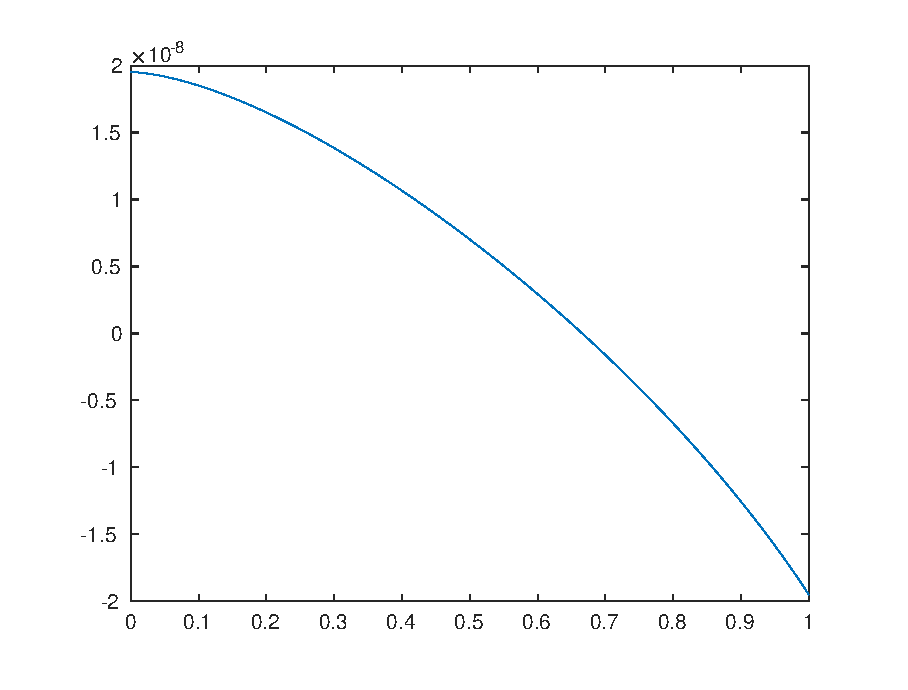
\includegraphics[width=0.8\linewidth]{figure/1-2-4.eps}
    \caption*{$n=4096$}
  \end{minipage}
\end{figure}

将数值解与真实解的误差用范数估计,并根据$n=16384$增加到$n=32768$时误差减小的倍数,估计各范数下的收敛阶,结果如下表。

\begin{table}[H]
  \centering
  \small
  \begin{tabular}{c|ccccccc|c}
  \textbf{$n$}        & 512                 & 1024                 & 2048                 & 4096                 & 8192                 & 16384                & 32768                & 收敛阶 \\ \hline
  $||\cdot||_1$      & $6.98\times 10^{-6}$ & $1.74\times 10^{-7}$ & $4.36\times 10^{-8}$ & $1.09\times 10^{-8}$ & $2.72\times 10^{-9}$ & $6.81\times 10^{-10}$ & $1.70\times 10^{-10}$ & $2.003$\\
  $||\cdot||_2$      & $7.95\times 10^{-6}$ & $1.98\times 10^{-7}$ & $4.96\times 10^{-8}$ & $1.24\times 10^{-8}$ & $3.10\times 10^{-9}$ & $7.75\times 10^{-10}$ & $1.93\times 10^{-10}$ & $2.003$\\
  $||\cdot||_\infty$ & $1.25\times 10^{-6}$ & $3.12\times 10^{-7}$ & $7.81\times 10^{-8}$ & $1.95\times 10^{-8}$ & $4.88\times 10^{-9}$ & $1.22\times 10^{-9}$ & $3.04\times 10^{-10}$ & $2.003$
  \end{tabular}
\end{table}

符合二阶收敛的理论结果。

\subsection{混合边值问题的求解、误差分析、收敛性分析}

考虑由精确解$u(x)=e^{\sin x}$导出的混合边值问题
\begin{equation}
  \left\{
    \begin{array}{l}
      -u''(x) = (\sin x-\cos^2 x)e^{\sin x},\quad x\in\Omega \\
      u(0)=1,\quad u'(1)=\cos 1\cdot e^{\sin 1}
    \end{array}
  \right. .
\end{equation}

我们用$n=512,1024,...,32768$的网格测试,使用FMG-Cycle,限制算子选择Full Operator,插值算子选择二次插值。当$n=512,...,4096$时,误差分布如下图所示。

\begin{figure}[H]
  \centering
  \begin{minipage}[t]{0.24\linewidth}
      \centering
      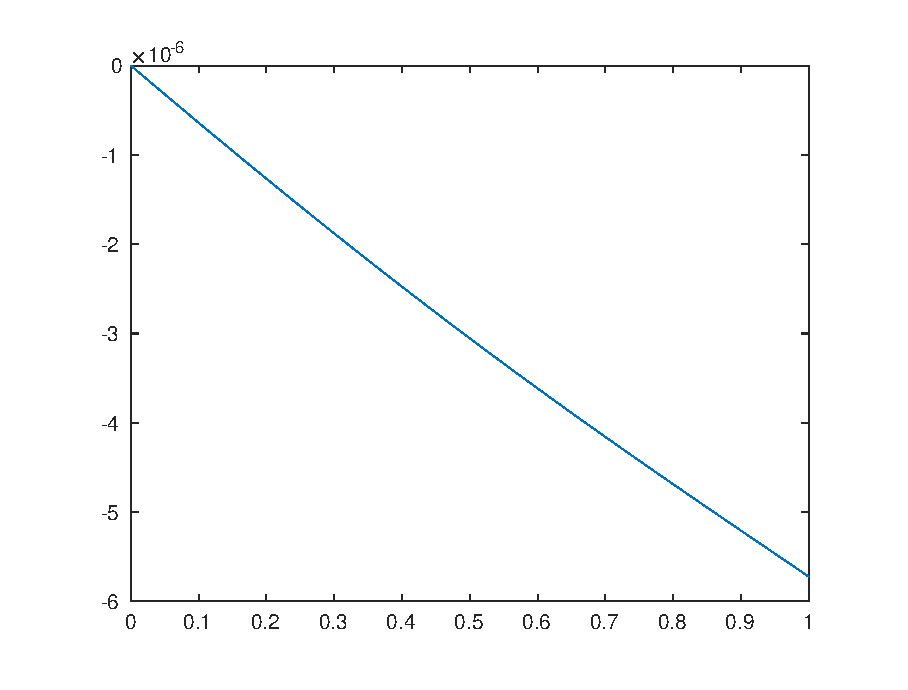
\includegraphics[width=0.8\linewidth]{figure/1-3-1.eps}
      \caption*{$n=512$}
  \end{minipage}
  \begin{minipage}[t]{0.24\linewidth}
    \centering
    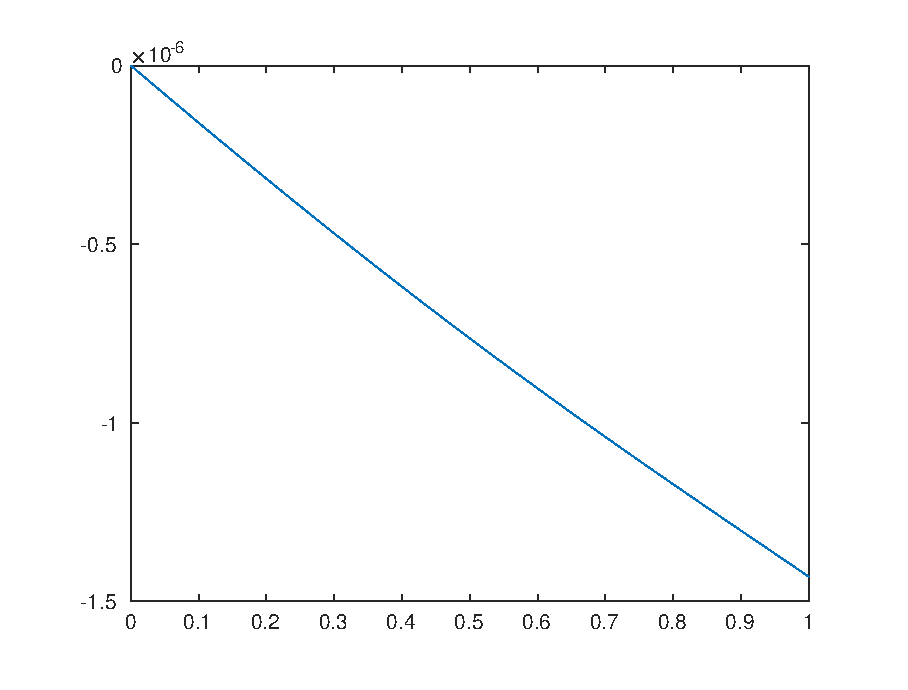
\includegraphics[width=0.8\linewidth]{figure/1-3-2.eps}
    \caption*{$n=1024$}
  \end{minipage}
  \begin{minipage}[t]{0.24\linewidth}
    \centering
    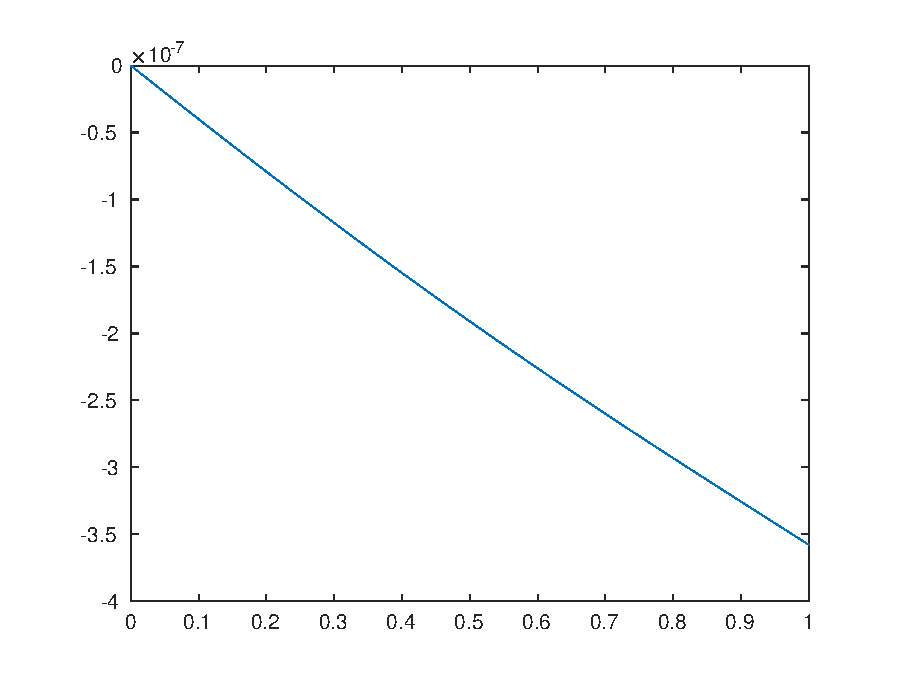
\includegraphics[width=0.8\linewidth]{figure/1-3-3.eps}
    \caption*{$n=2048$}
  \end{minipage}
  \begin{minipage}[t]{0.24\linewidth}
    \centering
    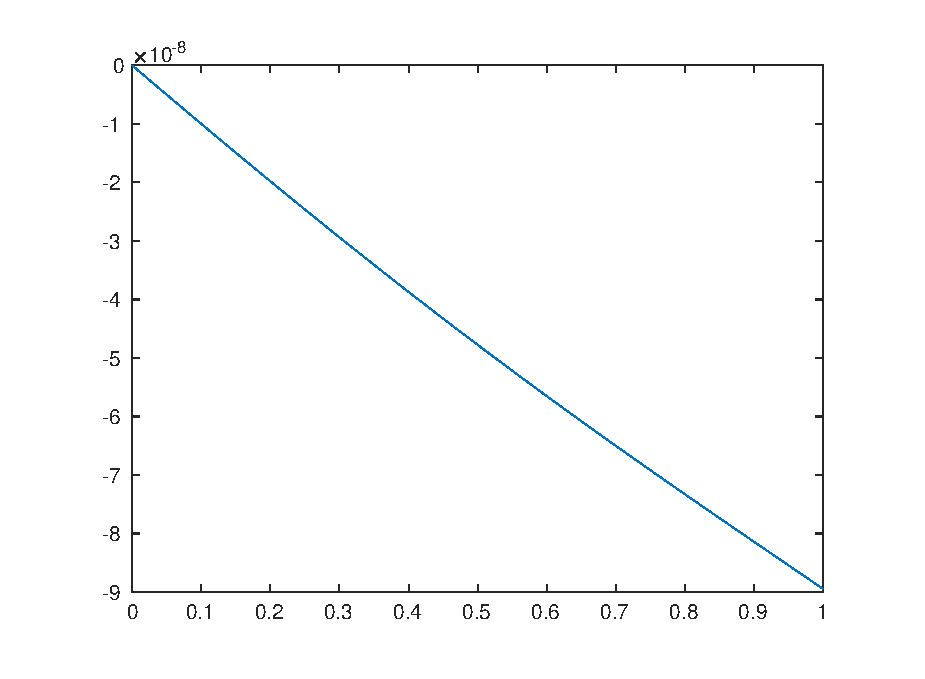
\includegraphics[width=0.8\linewidth]{figure/1-3-4.eps}
    \caption*{$n=4096$}
  \end{minipage}
\end{figure}

可以看到,格点越靠近Dirichlet条件下的边界,最终的计算误差越小。将数值解与真实解的误差用范数估计,并根据$n=16384$增加到$n=32768$时误差减小的倍数,估计各范数下的收敛阶,结果如下表。

\begin{table}[H]
  \centering
  \small
  \begin{tabular}{c|ccccccc|c}
  \textbf{$n$}        & 512                 & 1024                 & 2048                 & 4096                 & 8192                 & 16384                & 32768                & 收敛阶 \\ \hline
  $||\cdot||_1$      & $2.99\times 10^{-6}$ & $7.46\times 10^{-7}$ & $1.87\times 10^{-7}$ & $4.67\times 10^{-8}$ & $1.17\times 10^{-8}$ & $2.91\times 10^{-9}$ & $7.37\times 10^{-10}$ & $1.984$\\
  $||\cdot||_2$      & $3.41\times 10^{-6}$ & $8.53\times 10^{-7}$ & $2.13\times 10^{-7}$ & $5.33\times 10^{-8}$ & $1.33\times 10^{-8}$ & $3.33\times 10^{-9}$ & $8.42\times 10^{-10}$ & $1.984$\\
  $||\cdot||_\infty$ & $5.72\times 10^{-6}$ & $1.43\times 10^{-6}$ & $3.58\times 10^{-7}$ & $8.94\times 10^{-8}$ & $2.24\times 10^{-8}$ & $5.59\times 10^{-9}$ & $1.41\times 10^{-9}$ & $1.985$
  \end{tabular}
\end{table}

符合二阶收敛的理论结果。

\subsection{V-Cycle 与 FMG-Cycle 的对比}

本小节中,我们用Dirichlet边值问题(3.4)做测试。限制算子采用full-weighting,插值算子选择二次插值。

以$n=2^{15}$的网格为例,采用V-Cycle,每一步迭代的误差分布如下图。

\begin{figure}[H]
  \centering
  \begin{minipage}[t]{0.24\linewidth}
      \centering
      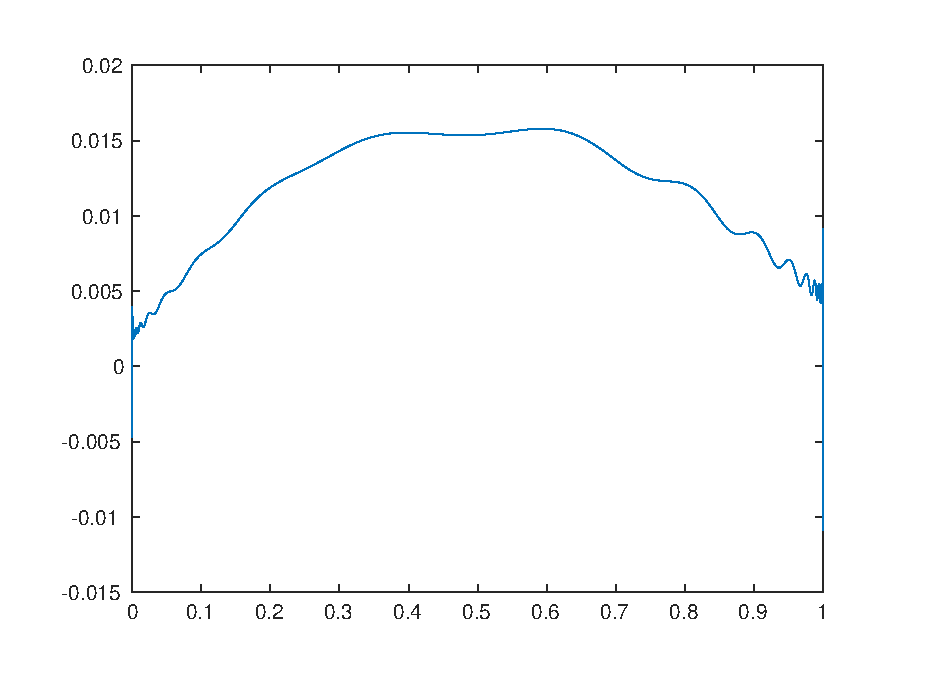
\includegraphics[width=0.9\linewidth]{figure/1-4-1.eps}
      \caption*{\small Iter 1 \\ $||\text{err}||_\infty=0.016$}
  \end{minipage}
  \begin{minipage}[t]{0.24\linewidth}
    \centering
    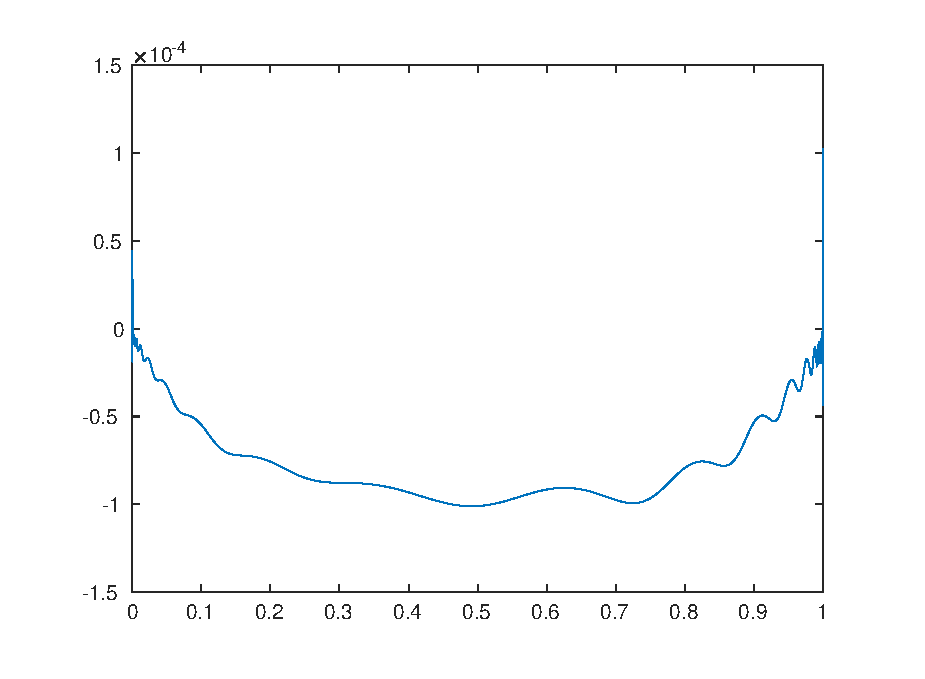
\includegraphics[width=0.9\linewidth]{figure/1-4-2.eps}
    \caption*{\small Iter 2 \\ $||\text{err}||_\infty=0.0001$}
  \end{minipage}
  \begin{minipage}[t]{0.24\linewidth}
    \centering
    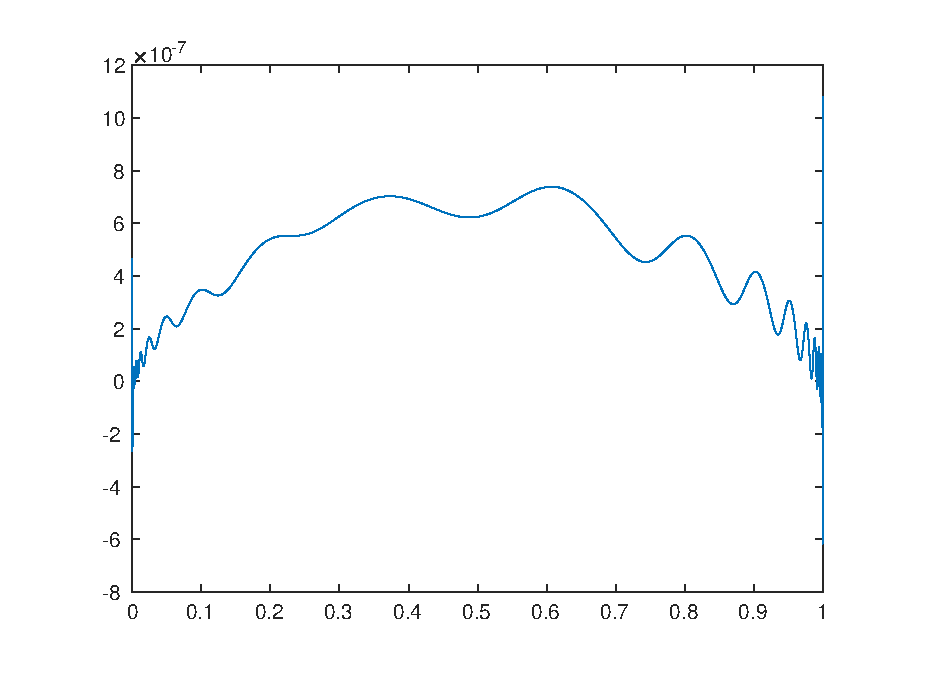
\includegraphics[width=0.9\linewidth]{figure/1-4-3.eps}
    \caption*{\small Iter 3 \\ $||\text{err}||_\infty=1.1\times 10^{-6}$}
  \end{minipage}
  \begin{minipage}[t]{0.24\linewidth}
    \centering
    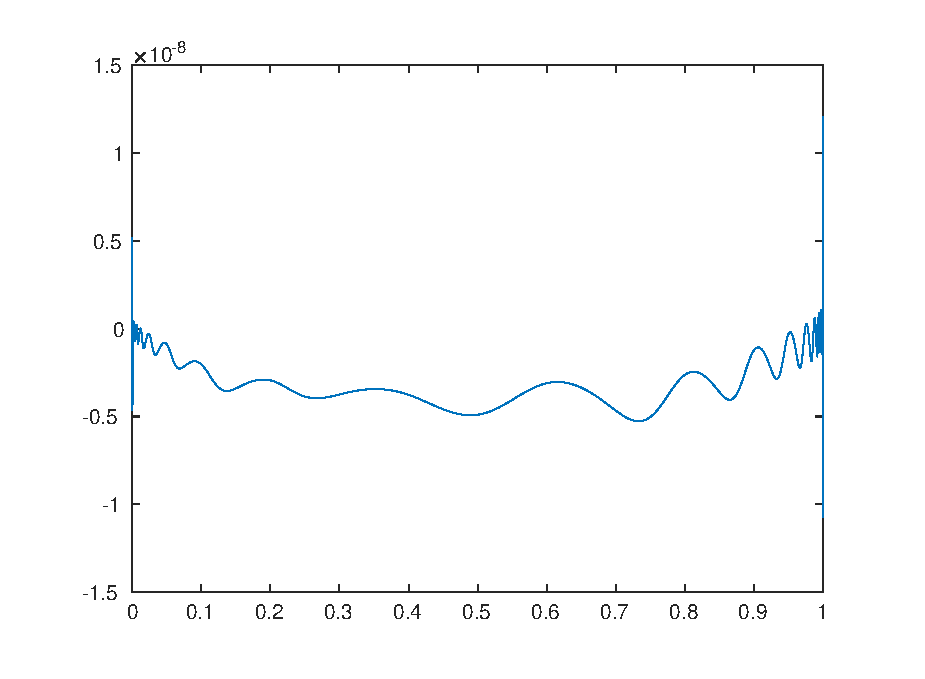
\includegraphics[width=0.9\linewidth]{figure/1-4-4.eps}
    \caption*{\small Iter 4 \\ $||\text{err}||_\infty=1.2\times 10^{-8}$}
  \end{minipage}
\end{figure}

采用FMG-Cycle,只需一步迭代即可收敛到离散误差,误差分布如下图。

\begin{figure}[H]
  \centering
  \begin{minipage}[t]{0.24\linewidth}
      \centering
      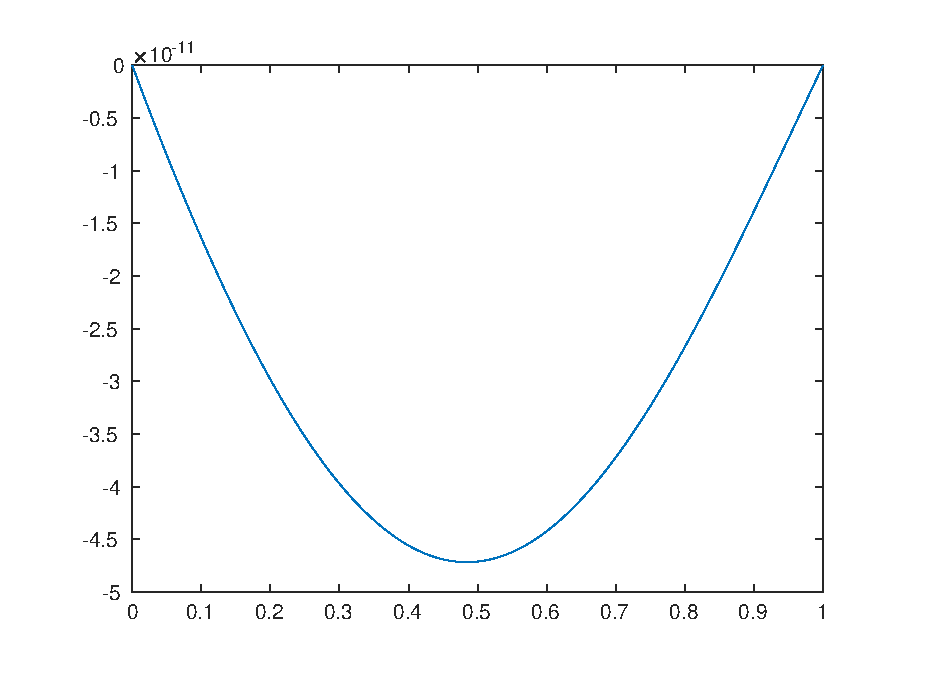
\includegraphics[width=0.9\linewidth]{figure/1-4-5.eps}
      \caption*{\small Iter 1 \\ $||\text{err}||_\infty=4.7\times 10^{-11}$}
  \end{minipage}
\end{figure}

我们使用不同大小的网格,取$n=2^{15},2^{16},2^{17},2^{18}$,用V-Cycle与FMG-Cycle分别迭代,达到离散误差即停。离散误差、迭代次数与求解时间如下表(误差均以无穷范数计)。

\begin{table}[H]
  \centering
  \small
  \begin{tabular}{c|ccccccc}
   $\mathbf{n}$      & $2^{15}$                   & $2^{16}$                   & $2^{17}$                  & $2^{18}$                    \\ \hline
离散误差$(\leq)$   & $4.80\times 10^{-11}$ & $1.18\times 10^{-11}$ & $2.95\times 10^{-12}$ & $7.37\times 10^{-13}$ \\
V-Cycle 迭代次数   & 7 & 7 & 8 & 7 \\
FMG-Cycle 迭代次数   & 1 & 1 & 1 & 1 \\
V-Cycle 耗时$(s)$  & 0.169 & 0.318 & 0.472 & 1.355 \\
FMG-Cycle 耗时$(s)$ & 0.098 & 0.182 & 0.308 & 0.625 
\end{tabular}
\end{table}

可以看出,FMG-Cycle只需一次迭代即可收敛。虽然V-Cycle的单次迭代比FMG-Cycle快,但需要的迭代次数太多。事实上,当$n$继续增大时,FMG-Cycle的快速收敛优势会更加明显,这里不再展示。

\subsection{限制算子与插值算子的选择测试}

本小节中,我们用Dirichlet边值问题(3.4)做测试。迭代方式选择FMG-Cycle,我们比较不同的限制算子与插值算子,设置如下四个实验组:
\begin{enumerate}[(i)]
  \item injection + 线性插值
  \item full-weighting + 线性插值
  \item injection + 二次插值
  \item full-weighting + 二次插值
\end{enumerate}

事实上,不管是怎样的算子组合,都能达到$O(h^2)$的精度,因此最终都能收敛至二阶离散误差。但是二次插值的精度是$O(h^3)$,因此我们有理由相信使用二次插值具有较快的收敛速度。

以$n=2^{15}$的网格为例,采用 injection + 线性插值 组合,每一步迭代的误差分布如下图。

\begin{figure}[H]
  \centering
  \begin{minipage}[t]{0.24\linewidth}
      \centering
      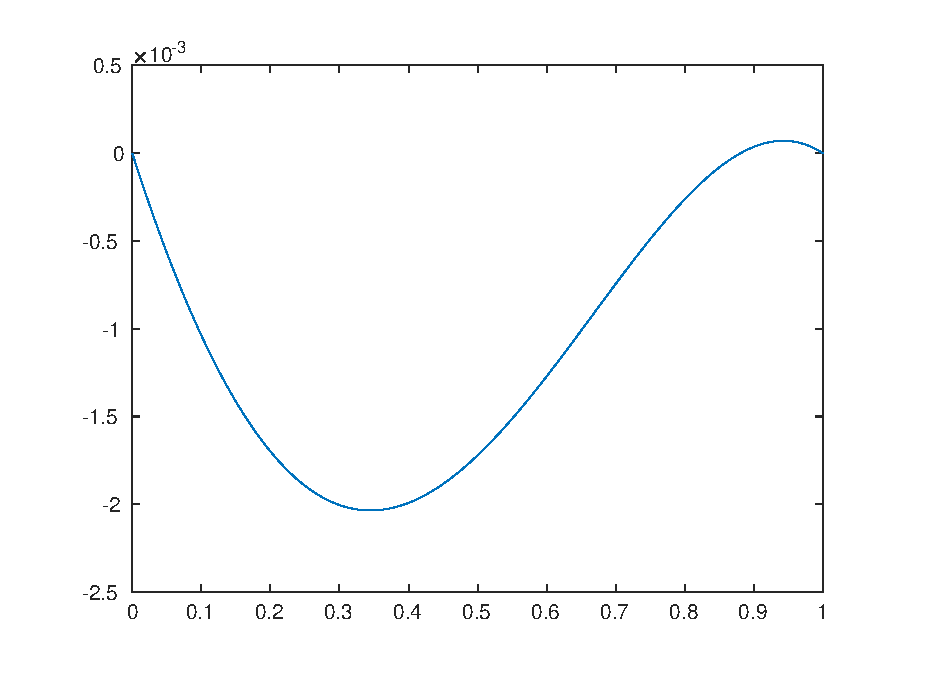
\includegraphics[width=0.9\linewidth]{figure/1-5-1.eps}
      \caption*{\small Iter 1 \\ $||\text{err}||_\infty=0.002$}
  \end{minipage}
  \begin{minipage}[t]{0.24\linewidth}
    \centering
    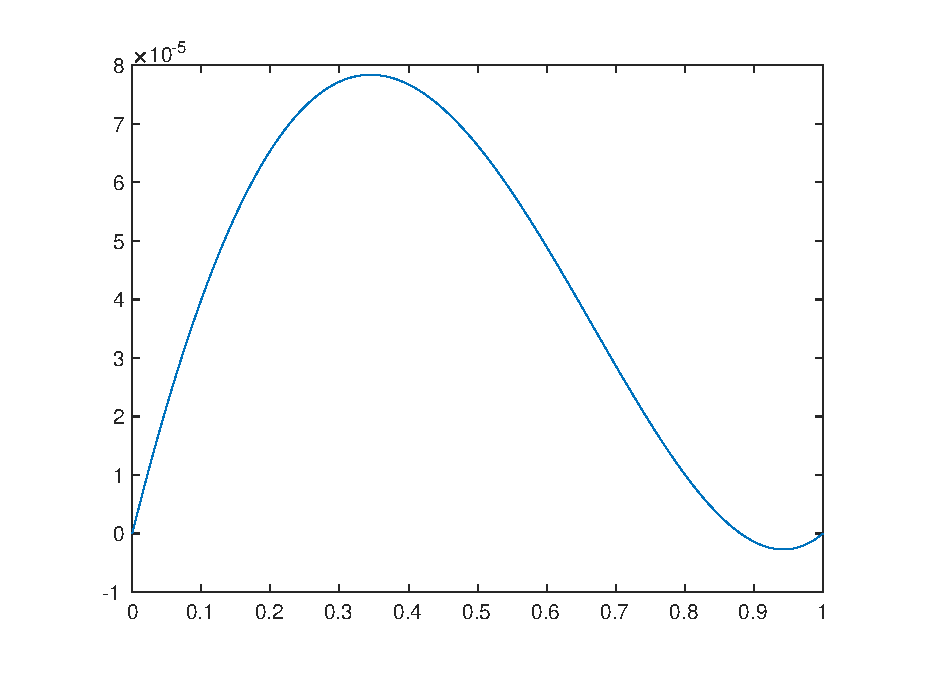
\includegraphics[width=0.9\linewidth]{figure/1-5-2.eps}
    \caption*{\small Iter 2 \\ $||\text{err}||_\infty=7.8\times 10^{-5}$}
  \end{minipage}
  \begin{minipage}[t]{0.24\linewidth}
    \centering
    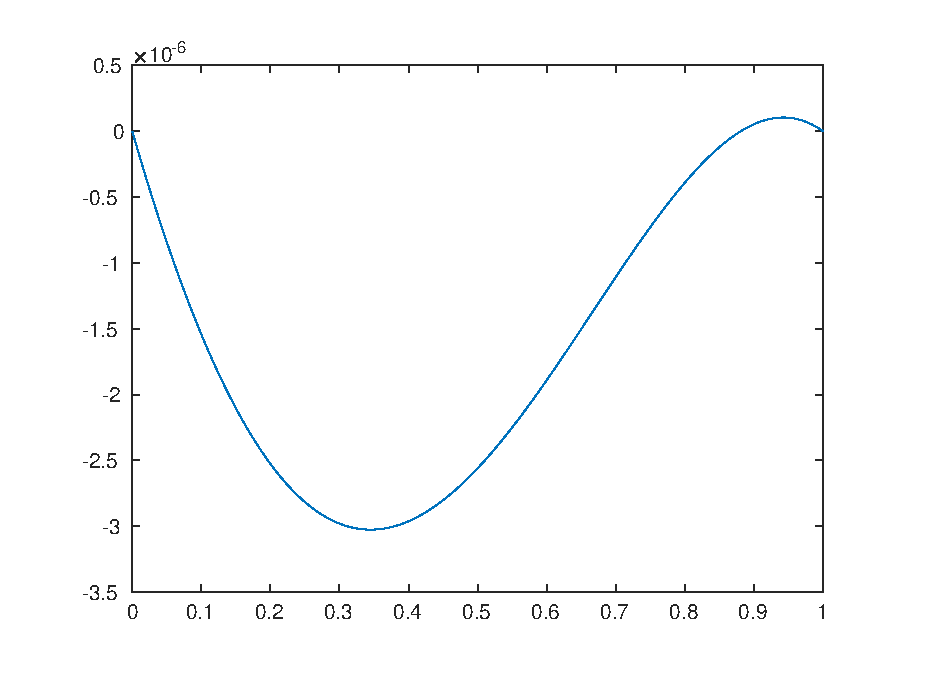
\includegraphics[width=0.9\linewidth]{figure/1-5-3.eps}
    \caption*{\small Iter 3 \\ $||\text{err}||_\infty=3.0\times 10^{-6}$}
  \end{minipage}
  \begin{minipage}[t]{0.24\linewidth}
    \centering
    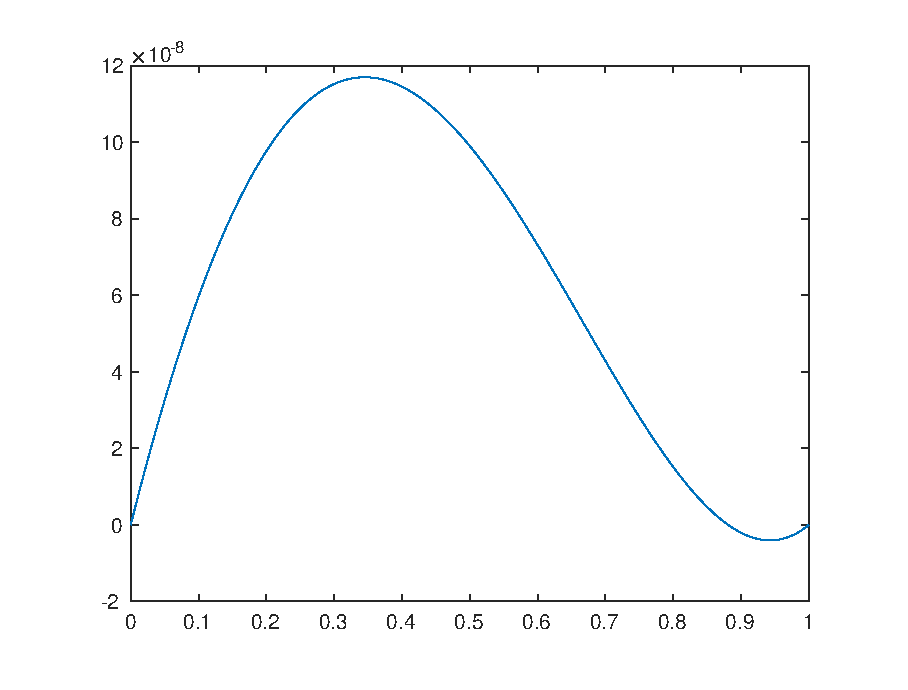
\includegraphics[width=0.9\linewidth]{figure/1-5-4.eps}
    \caption*{\small Iter 4 \\ $||\text{err}||_\infty=1.2\times 10^{-7}$}
  \end{minipage}
\end{figure}

采用 full-weighting + 线性插值 组合,每一步迭代的误差分布如下图。

\begin{figure}[H]
  \centering
  \begin{minipage}[t]{0.24\linewidth}
      \centering
      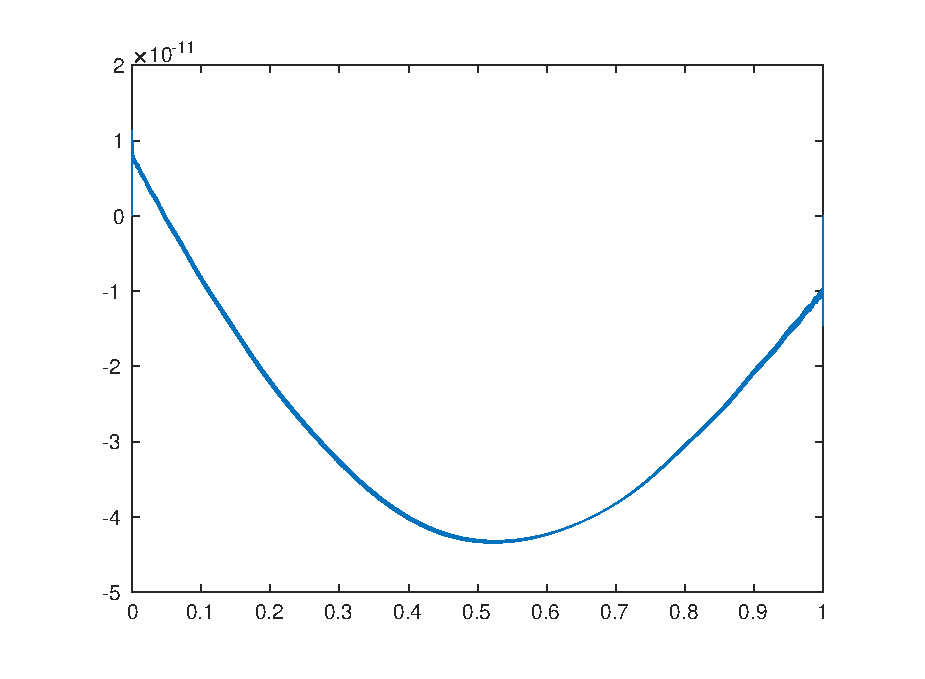
\includegraphics[width=0.9\linewidth]{figure/1-5-5.eps}
      \caption*{\small Iter 1 \\ $||\text{err}||_\infty=4.4\times 10^{-11}$}
  \end{minipage}
  \begin{minipage}[t]{0.24\linewidth}
    \centering
    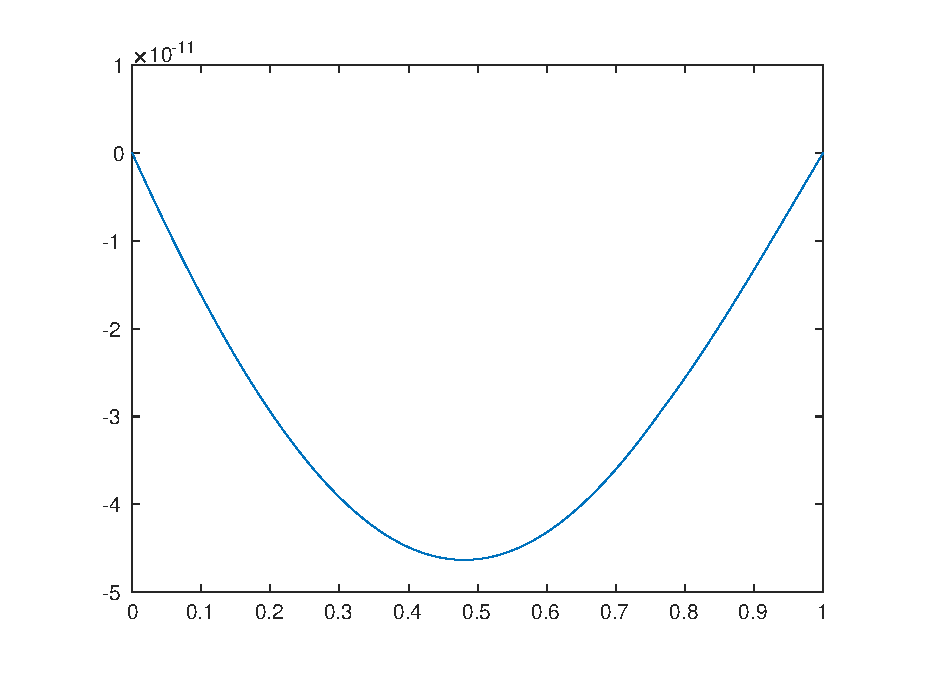
\includegraphics[width=0.9\linewidth]{figure/1-5-6.eps}
    \caption*{\small Iter 2 \\ $||\text{err}||_\infty=4.6\times 10^{-11}$}
  \end{minipage}
\end{figure}

注意,上述第1步到第2步发生了误差增大。其实这是真实误差增大,方程组的求解误差仍在减小,并不能据此认为第1步的结果更好,第1步得到一个比较小的真实误差纯属巧合。

采用 injection + 二次插值 组合,每一步迭代的误差分布如下图。

\begin{figure}[H]
  \centering
  \begin{minipage}[t]{0.24\linewidth}
      \centering
      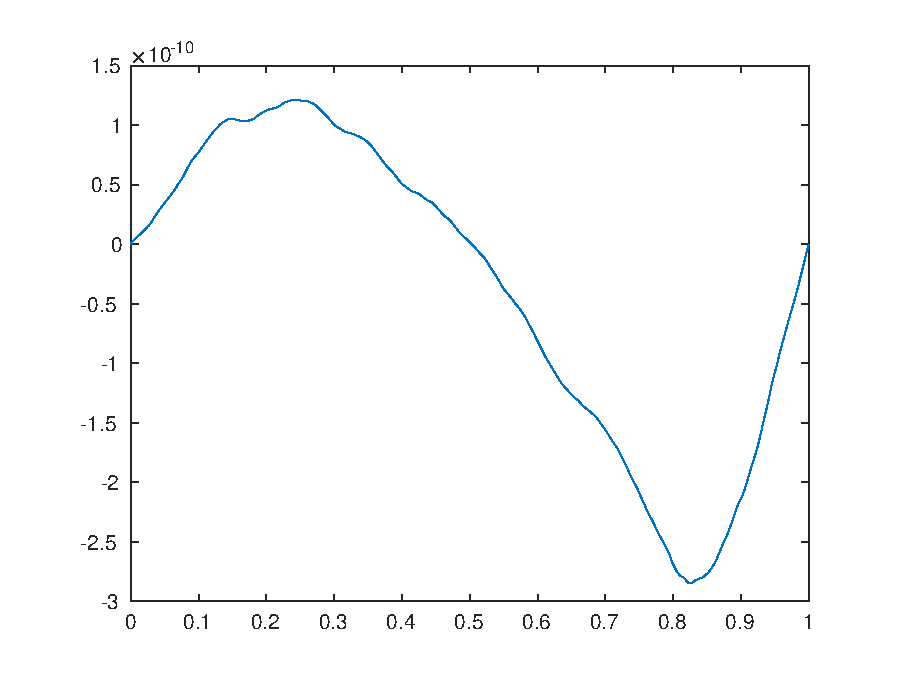
\includegraphics[width=0.9\linewidth]{figure/1-5-7.eps}
      \caption*{\small Iter 1 \\ $||\text{err}||_\infty=2.8\times 10^{-10}$}
  \end{minipage}
  \begin{minipage}[t]{0.24\linewidth}
    \centering
    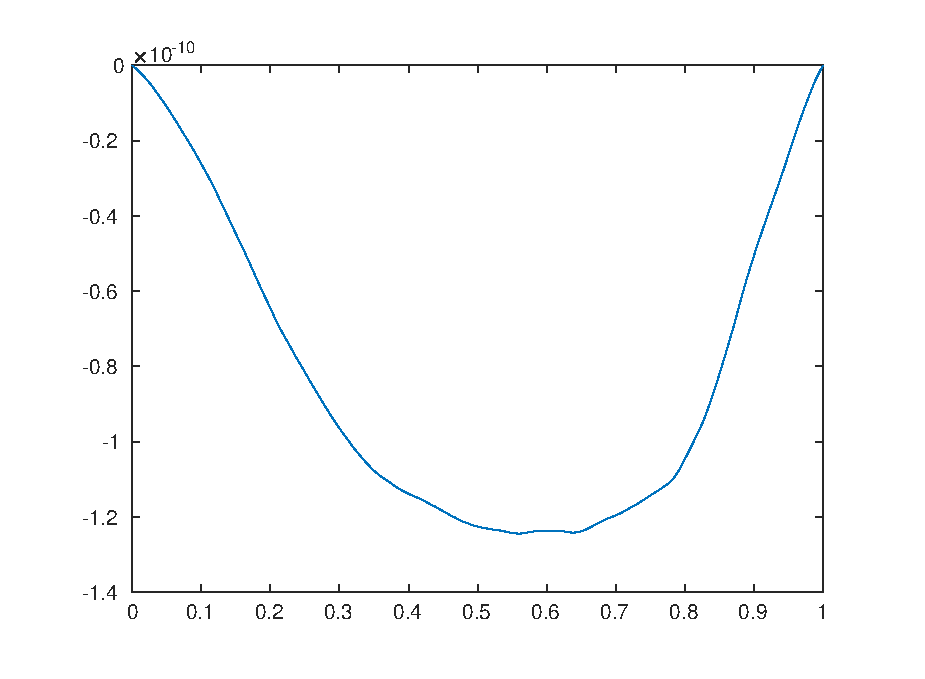
\includegraphics[width=0.9\linewidth]{figure/1-5-8.eps}
    \caption*{\small Iter 2 \\ $||\text{err}||_\infty=1.2\times 10^{-10}$}
  \end{minipage}
  \begin{minipage}[t]{0.24\linewidth}
    \centering
    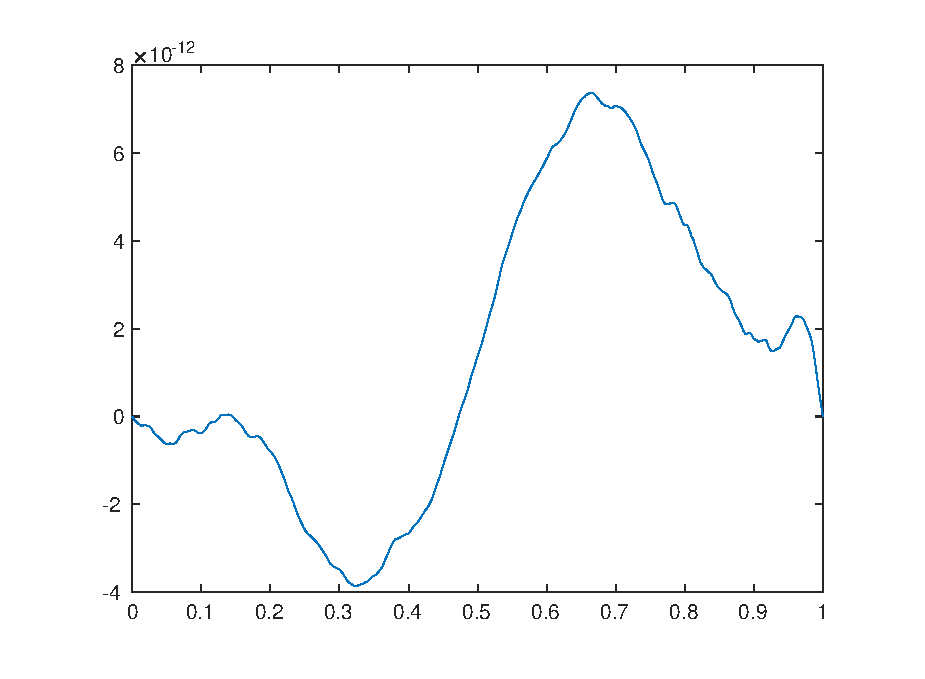
\includegraphics[width=0.9\linewidth]{figure/1-5-9.eps}
    \caption*{\small Iter 3 \\ $||\text{err}||_\infty=7.3\times 10^{-12}$}
  \end{minipage}
  \begin{minipage}[t]{0.24\linewidth}
    \centering
    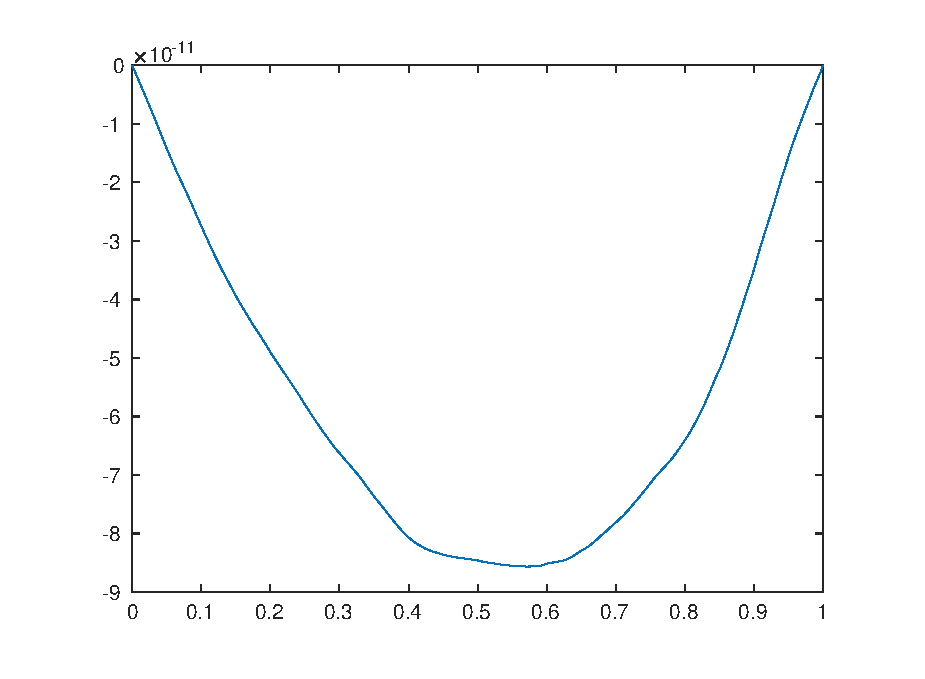
\includegraphics[width=0.9\linewidth]{figure/1-5-10.eps}
    \caption*{\small Iter 4 \\ $||\text{err}||_\infty=8.6\times 10^{-11}$}
  \end{minipage}
\end{figure}

采用 full-weighting + 二次插值 组合,一步迭代即可收敛,误差分布如下图。

\begin{figure}[H]
  \centering
  \begin{minipage}[t]{0.24\linewidth}
      \centering
      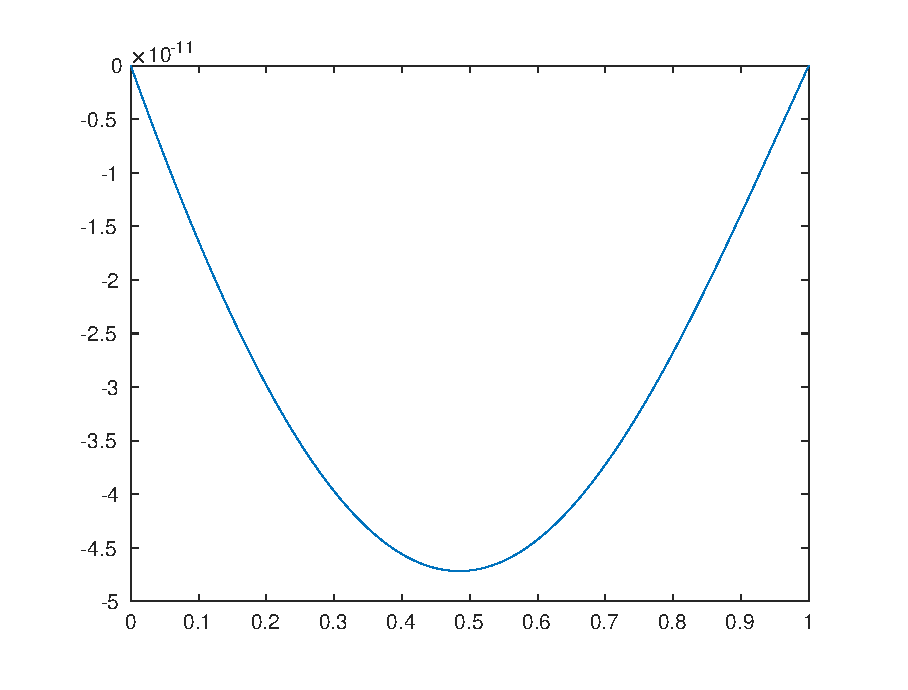
\includegraphics[width=0.9\linewidth]{figure/1-5-11.eps}
      \caption*{\small Iter 1 \\ $||\text{err}||_\infty=4.7\times 10^{-11}$}
  \end{minipage}
\end{figure}

下面我们取$n=2^{15},...,2^{18}$的网格测试,记录各实验组达到离散误差所需的迭代次数,结果如下表。

\begin{table}[H]
  \centering
  \small
  \begin{tabular}{c|ccccccc}
   $\mathbf{n}$      & $2^{15}$                   & $2^{16}$                   & $2^{17}$                  & $2^{18}$                    \\ \hline
离散误差$(\leq)$   & $4.80\times 10^{-11}$ & $1.18\times 10^{-11}$ & $2.95\times 10^{-12}$ & $7.37\times 10^{-13}$ \\
injection + 线性插值 迭代次数        & 10 & 9 & 9 & 10 \\
full-weighting + 线性插值 迭代次数   & 3  & 5 & 2 & 2 \\
injection + 二次插值 迭代次数        & 6  & 4 & 2 & 3 \\
full-weighting + 二次插值 迭代次数   & 1  & 1 & 1 & 1 \\
\end{tabular}
\end{table}

由结果可见,所有组合最终都能收敛。其中 full-weighting + 二次插值 是收敛最快的组合,而 injection + 一次插值 是收敛最慢的组合。另外两个组合没有明显的优劣。

\subsection{求解精度的极限测试}

在这一节中,我们求解Dirichlet边值问题(3.4),测试极限的求解精度。从$n=2^{16}$开始,采用最佳配置,即FMG-Cycle + full-weighting + 二次插值。测试结果如下:

\begin{table}[H]
  \centering
  \small
  \begin{tabular}{c|cccccc}
  \hline
    \textbf{$n$}                 & $2^{16}$                 & $2^{17}$                 & $2^{18}$                 & $2^{19}$                & $2^{20}$                 & $2^{21}$              \\ \hline
  $||\text{err}||_1$      & $7.58\times 10^{-12}$ & $1.90\times 10^{-12}$ & $4.74\times 10^{-13}$ & $1.18\times 10^{-13}$ & $2.97\times 10^{-14}$ & $7.54\times 10^{-15}$  \\
  $||\text{err}||_\infty$      & $1.18\times 10^{-11}$ & $2.95\times 10^{-12}$ & $7.37\times 10^{-13}$ & $1.85\times 10^{-13}$ & $4.61\times 10^{-14}$ & $1.18\times 10^{-14}$  \\
  求解时间(秒)                 & 0.214 & 0.402 & 0.813 & 1.957 & 4.444 & 9.488 \\ \hline 
  \textbf{$n$}                 & $2^{22}$                 & $2^{23}$                 & $2^{24}$                 & $2^{25}$             \\ \hline
  $||\text{err}||_1$      & $1.94\times 10^{-15}$ & $5.48\times 10^{-15}$ & $2.01\times 10^{-16}$ & $1.14\times 10^{-16}$ \\
  $||\text{err}||_\infty$      & $3.11\times 10^{-15}$ & $1.11\times 10^{-15}$ & $4.44\times 10^{-16}$ & $4.44\times 10^{-16}$  \\
  求解时间(秒)                 & 20.035 & 56.561 & 86.955 & 236.812 \\ \hline
  \end{tabular}
\end{table}

我们可以发现,从$n=2^{22}$开始,网格变得巨大,求解时间开始肉眼可见地增长。我们最大的测试网格达到了$2^{25}$,求解精度接近\verb|double|的机器精度。但令人遗憾的是,也正是从$n=2^{22}$开始,网格每增大一倍,求解误差并不能下降到原先的$\frac{1}{4}$倍,这没有印证理论的二阶收敛。

我们认为巨大网格下收敛阶数难以保持的主要原因是,当$n$足够大时,离散误差$O(h^2)$接近机器精度,由于浮点数运算的误差累积会对结果产生影响,这个影响放在$O(h^2)$尺度下就显得相当大,导致收敛阶无规律。

\newpage

\chapter{二维规则区域中的BVP}

\section{设计要点}

\subsection{二维区域的线性插值}

我们将细网格上的点分为四种情况,分别插值:
\begin{itemize}
  \item 在粗网格格点上。此时直接等于粗网格点上的值。
  \item 在粗网格的某条水平线上。此时该点值等与左右两粗网格格点值的平均。
  \item 在粗网格的某条竖直线上。此时该点值等与上下两粗网格格点值的平均。
  \item 不在粗网格线上。此时周围有四个粗网格格点,该点点值等于这四个粗网格格点值的平均。
\end{itemize}

\subsection{二维区域的二次插值}

仍然将点分为四类。事实上,在粗网格线上的点可以使用一维的二次插值公式,唯一需要考虑的就是不在粗网格线上的点。考虑点$P_0=G^h(2i+1,2j+1)$,做一次二维二次插值需要六个点,取:
\begin{align*}
  P_1&=G^h(i,j) & P_2&=G^h(i,j+1) & P_3&=G^h(i,j+2)\\
  P_4&=G^h(i+1,j) & P_5&=G^h(i+1,j+1) & P_6&=G^h(i+1,j+2)
\end{align*}

以这六个点的点值,通过待定系数法确定一个二维二次多项式$Q(x,y)=A+Bx+Cy+Dx^2+Exy+Fy^2$,再将$P_0$代入求得点值。结果为:
\begin{equation*}
  u(P_0)=\frac{1}{2}u(P_2)-\frac{1}{8}u(P_3)+\frac{1}{2}u(P_4)+\frac{1}{4}u(P_5)-\frac{1}{8}u(P_6).
\end{equation*}

这个形式不够对称,因此我们更换$P_1,...,P_6$的选取,重复上述过程三次,将每次得到的系数在各点上相加,并乘上$\frac{1}{4}$,得到对称的二次插值公式,各点插值系数如下图所示。
\begin{figure}[H]
  \centering
  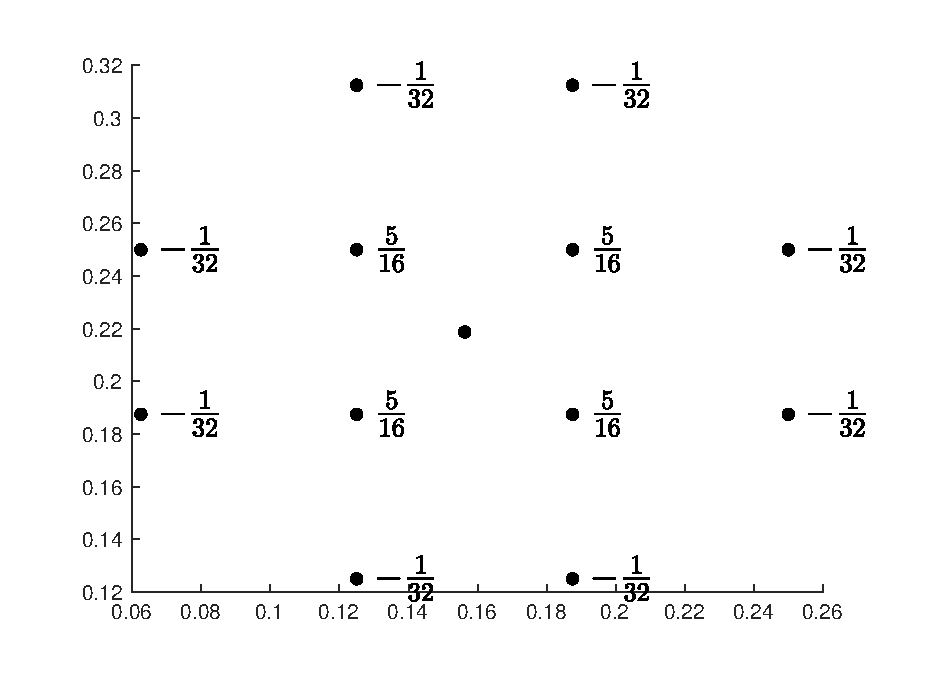
\includegraphics[width=0.4\textwidth]{figure/2-1.eps}
\end{figure}

注意,上述对称的形式在边界附近会有越界问题,此时应该做特殊处理,牺牲一些对称性。

\section{数值实验}

\subsection{Dirichlet边值问题的求解、误差分析、收敛性分析}

考虑由精确解$u(x,y)=e^{\sin x+y}$导出的Dirichlet边值问题
\begin{equation}
  \left\{
    \begin{array}{l}
      -\Delta u = -(1-\sin x+\cos^2 x)e^{\sin x + y},\quad x\in\Omega \\
      u|_{\partial \Omega}=e^{\sin x + y}
    \end{array}
  \right. .
\end{equation}

我们用$n=16,32,64,128,256,512,1024$的网格测试,使用V-Cycle,限制算子选择Full Operator,插值算子选择线性插值。当$n=16,32,64,128$时,误差分布如下图所示。
\begin{figure}[H]
  \centering
  \begin{minipage}[t]{0.24\linewidth}
      \centering
      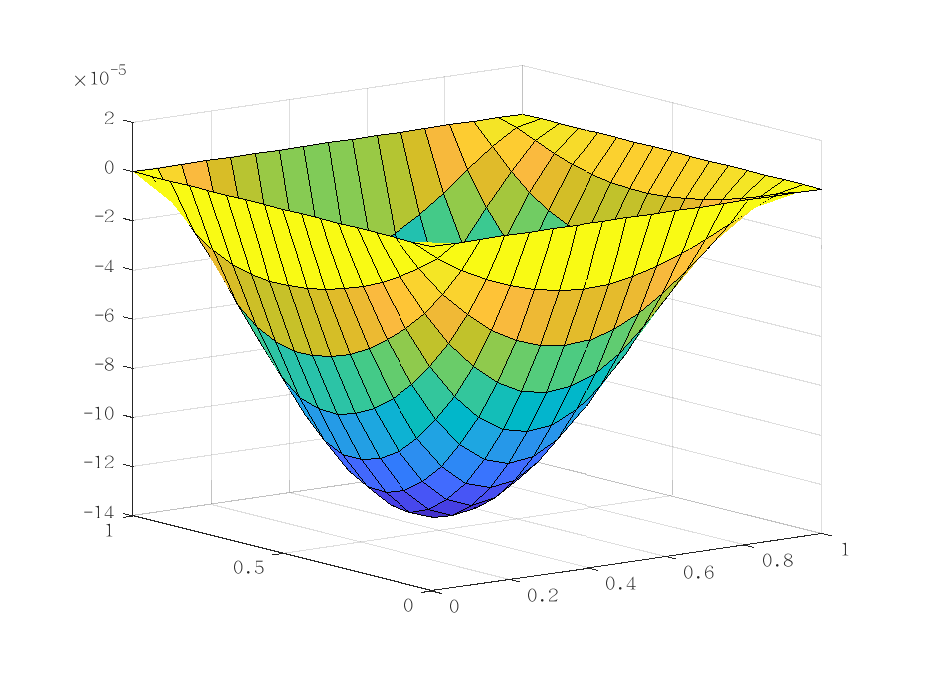
\includegraphics[width=0.95\linewidth]{figure/2-1-1.eps}
      \caption*{$n=16$}
  \end{minipage}
  \begin{minipage}[t]{0.24\linewidth}
    \centering
    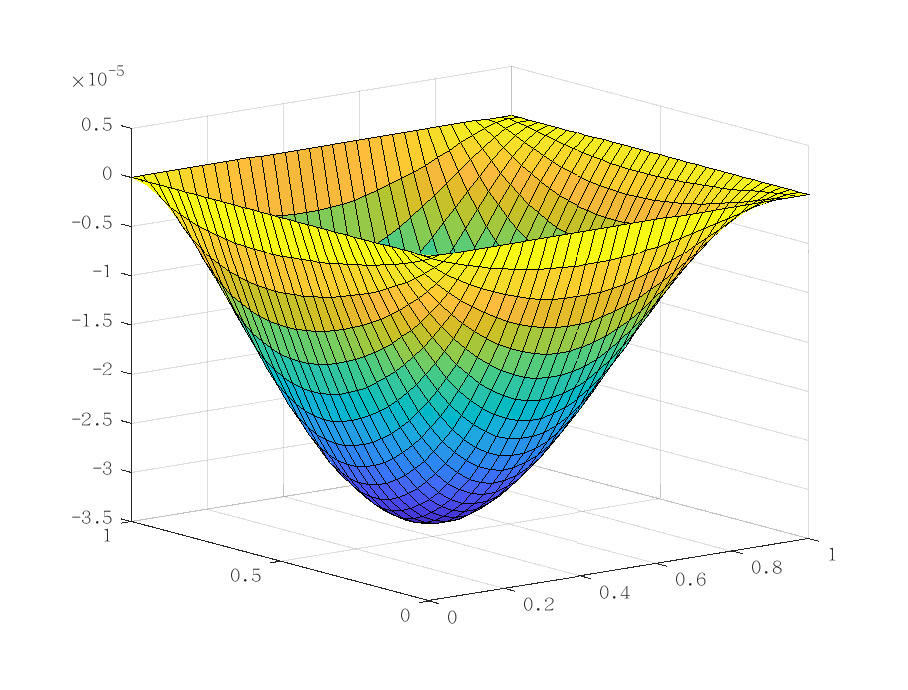
\includegraphics[width=0.95\linewidth]{figure/2-1-2.eps}
    \caption*{$n=32$}
  \end{minipage}
  \begin{minipage}[t]{0.24\linewidth}
    \centering
    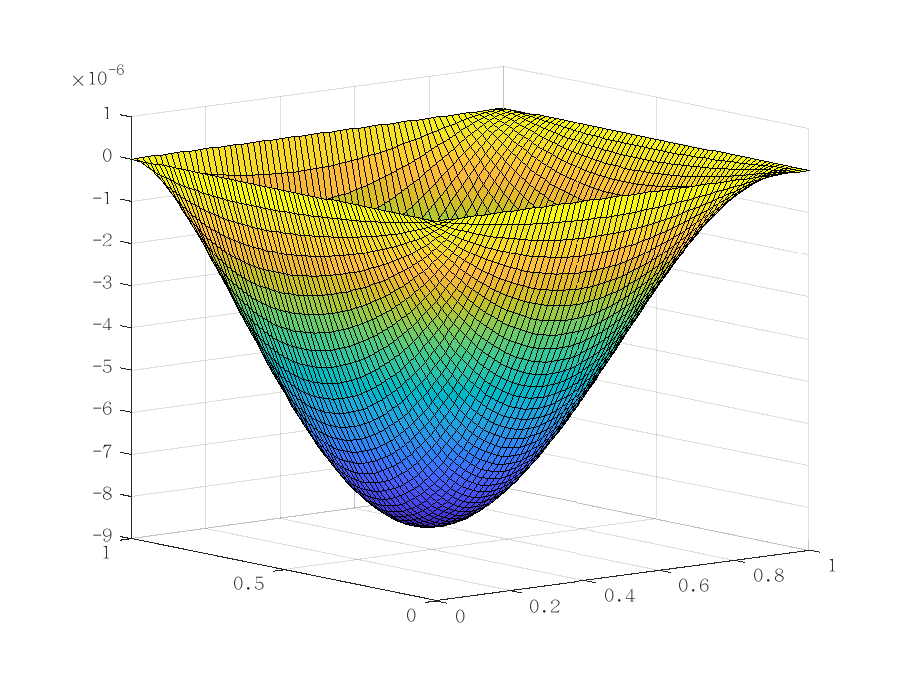
\includegraphics[width=0.95\linewidth]{figure/2-1-3.eps}
    \caption*{$n=64$}
  \end{minipage}
  \begin{minipage}[t]{0.24\linewidth}
    \centering
    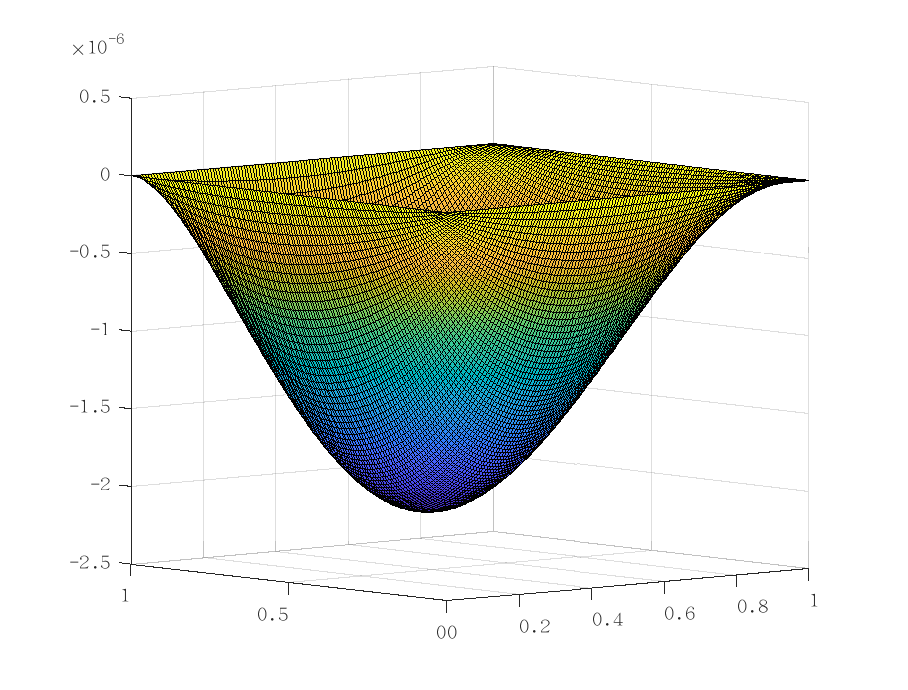
\includegraphics[width=0.95\linewidth]{figure/2-1-4.eps}
    \caption*{$n=128$}
  \end{minipage}
\end{figure}

可以看到,在Dirichlet条件下,格点越靠近边界,最终的计算误差越小。将数值解与真实解的误差用范数估计,并根据$n=512$增加到$n=1024$时误差减小的倍数,估计各范数下的收敛阶,结果如下表。

\begin{table}[H]
  \centering
  \small
  \begin{tabular}{c|ccccccc|c}
  \textbf{$n$}        & 16                   & 32                   & 64                   & 128                  & 256                  & 512                  & 1024                  & 收敛阶 \\ \hline
  $||\cdot||_1$      & $5.13\times 10^{-5}$ & $1.37\times 10^{-5}$ & $3.54\times 10^{-6}$ & $8.98\times 10^{-7}$ & $2.26\times 10^{-7}$ & $5.68\times 10^{-8}$ & $1.42\times 10^{-8}$ & $2.000$\\
  $||\cdot||_2$      & $6.71\times 10^{-5}$ & $1.73\times 10^{-5}$ & $4.40\times 10^{-6}$ & $1.11\times 10^{-6}$ & $2.78\times 10^{-7}$ & $6.97\times 10^{-8}$ & $1.74\times 10^{-8}$ & $2.002$\\
  $||\cdot||_\infty$ & $1.38\times 10^{-4}$ & $3.45\times 10^{-5}$ & $8.62\times 10^{-6}$ & $2.16\times 10^{-6}$ & $5.39\times 10^{-7}$ & $1.35\times 10^{-7}$ & $3.37\times 10^{-8}$ & $1.997$
  \end{tabular}
\end{table}

符合二阶收敛的理论结果。

\subsection{Neumann边值问题的求解、误差分析、收敛性分析}

考虑由精确解$u(x,y)=e^{\sin x+y}$导出的Neumann边值问题
\begin{equation}
  \left\{
    \begin{array}{l}
      -\Delta u = -(1-\sin x+\cos^2 x)e^{\sin x + y},\quad x\in\Omega, \\
      \frac{\partial u}{\partial \mathbf{n}}|_{x=0}=-e^{y},\\
      \frac{\partial u}{\partial \mathbf{n}}|_{x=1}=\cos 1 \cdot e^{\sin 1 + y},\\
      \frac{\partial u}{\partial \mathbf{n}}|_{y=0}=-e^{\sin x},\\
      \frac{\partial u}{\partial \mathbf{n}}|_{y=1}=e^{\sin x+1}
    \end{array}
  \right. .
\end{equation}

我们用$n=16,32,64,128,256,512,1024$的网格测试,使用V-Cycle,限制算子选择Full Operator,插值算子选择二次插值。当$n=16,32,64,128$时,误差分布如下图所示。
\begin{figure}[H]
  \centering
  \begin{minipage}[t]{0.24\linewidth}
      \centering
      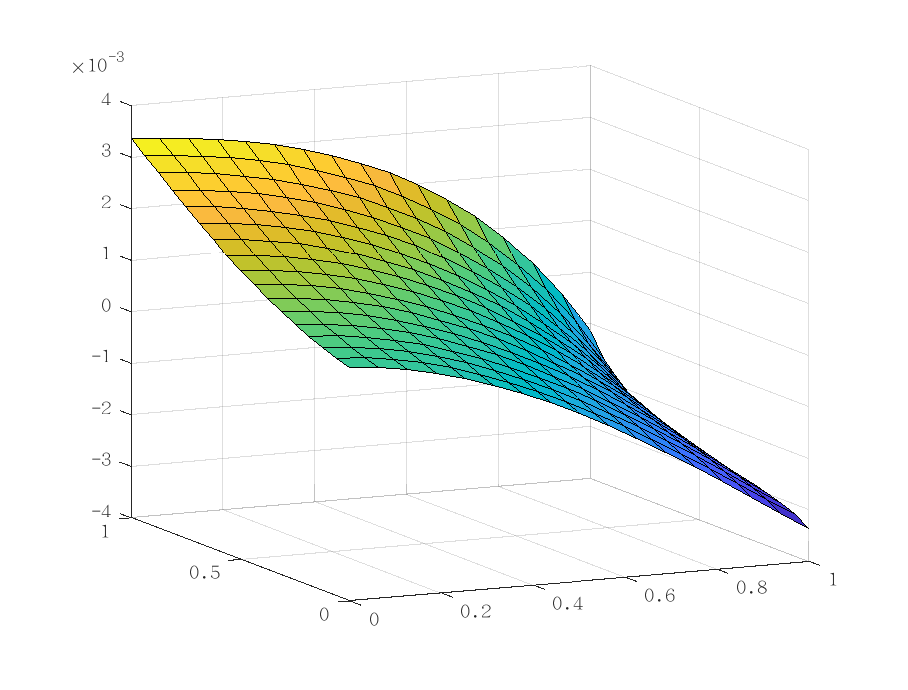
\includegraphics[width=0.95\linewidth]{figure/2-2-1.eps}
      \caption*{$n=16$}
  \end{minipage}
  \begin{minipage}[t]{0.24\linewidth}
    \centering
    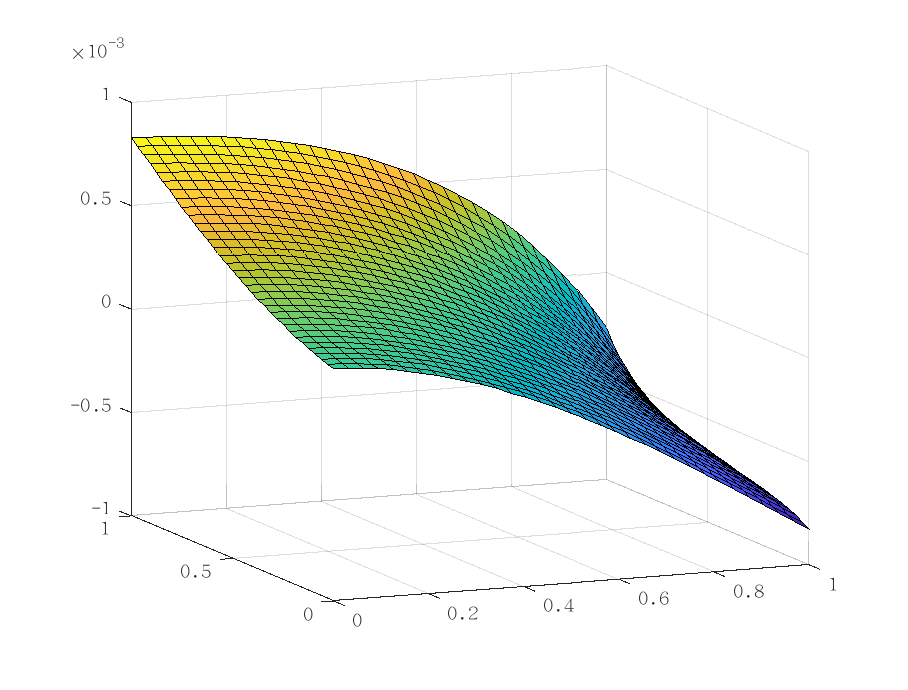
\includegraphics[width=0.95\linewidth]{figure/2-2-2.eps}
    \caption*{$n=32$}
  \end{minipage}
  \begin{minipage}[t]{0.24\linewidth}
    \centering
    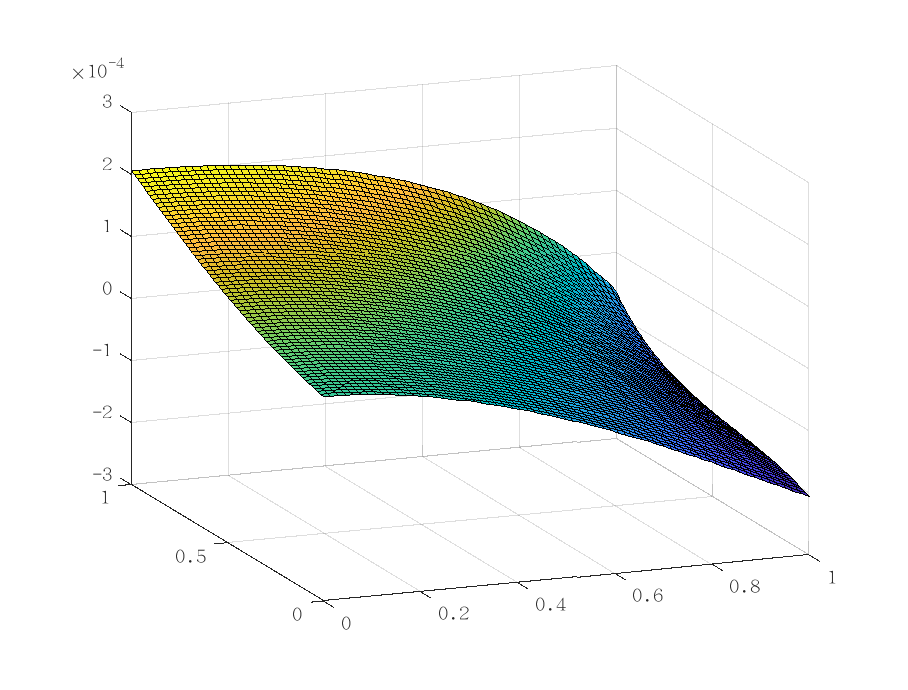
\includegraphics[width=0.95\linewidth]{figure/2-2-3.eps}
    \caption*{$n=64$}
  \end{minipage}
  \begin{minipage}[t]{0.24\linewidth}
    \centering
    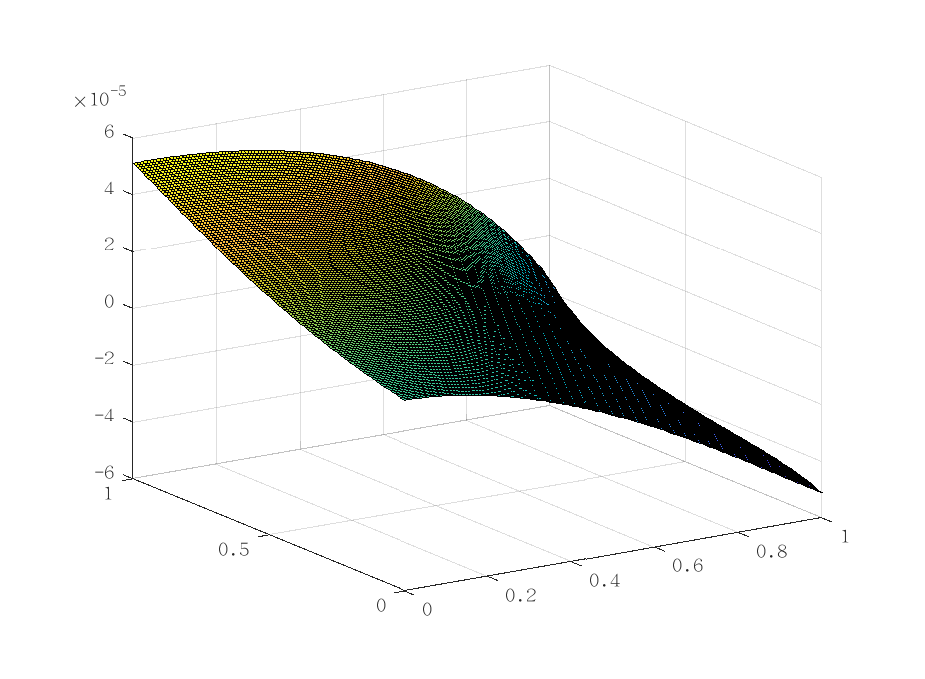
\includegraphics[width=0.95\linewidth]{figure/2-2-4.eps}
    \caption*{$n=128$}
  \end{minipage}
\end{figure}

将数值解与真实解的误差用范数估计,并根据$n=512$增加到$n=1024$时误差减小的倍数,估计各范数下的收敛阶,结果如下表。

\begin{table}[H]
  \centering
  \small
  \begin{tabular}{c|ccccccc|c}
  \textbf{$n$}        & 16                   & 32                   & 64                   & 128                  & 256                  & 512                  & 1024                  & 收敛阶 \\ \hline
  $||\cdot||_1$      & $1.36\times 10^{-3}$ & $3.26\times 10^{-4}$ & $7.99\times 10^{-5}$ & $1.98\times 10^{-5}$ & $4.92\times 10^{-6}$ & $1.22\times 10^{-6}$ & $3.06\times 10^{-7}$ & $1.995$\\
  $||\cdot||_2$      & $1.62\times 10^{-3}$ & $3.91\times 10^{-4}$ & $9.58\times 10^{-5}$ & $2.37\times 10^{-5}$ & $5.90\times 10^{-6}$ & $1.47\times 10^{-6}$ & $3.67\times 10^{-7}$ & $2.002$\\
  $||\cdot||_\infty$ & $3.36\times 10^{-3}$ & $8.28\times 10^{-4}$ & $2.06\times 10^{-4}$ & $5.12\times 10^{-5}$ & $1.28\times 10^{-5}$ & $3.19\times 10^{-6}$ & $7.97\times 10^{-7}$ & $2.001$
  \end{tabular}
\end{table}

符合二阶收敛的理论结果。

\subsection{混合边值问题的求解、误差分析、收敛性分析}

考虑由精确解$u(x,y)=e^{\sin x+y}$导出的混合边值问题
\begin{equation}
  \left\{
    \begin{array}{l}
      -\Delta u = -(1-\sin x+\cos^2 x)e^{\sin x + y},\quad x\in\Omega, \\
      u|_{x=0}=e^{y},\\
      u|_{x=1}=e^{y+\sin 1},\\
      \frac{\partial u}{\partial \mathbf{n}}|_{y=0}=-e^{\sin x},\\
      \frac{\partial u}{\partial \mathbf{n}}|_{y=1}=e^{\sin x+1}
    \end{array}
  \right. .
\end{equation}

我们用$n=16,32,64,128,256,512,1024$的网格测试,使用FMG-Cycle,限制算子选择Injection,插值算子选择线性插值。当$n=16,32,64,128$时,误差分布如下图所示。

\begin{figure}[H]
  \centering
  \begin{minipage}[t]{0.24\linewidth}
      \centering
      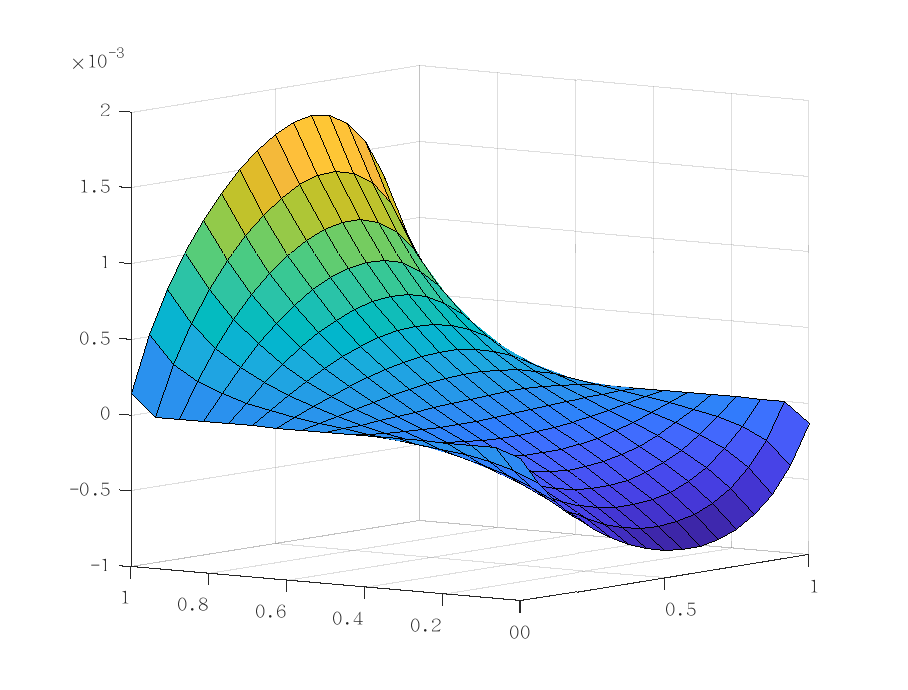
\includegraphics[width=0.8\linewidth]{figure/2-3-1.eps}
      \caption*{$n=16$}
  \end{minipage}
  \begin{minipage}[t]{0.24\linewidth}
    \centering
    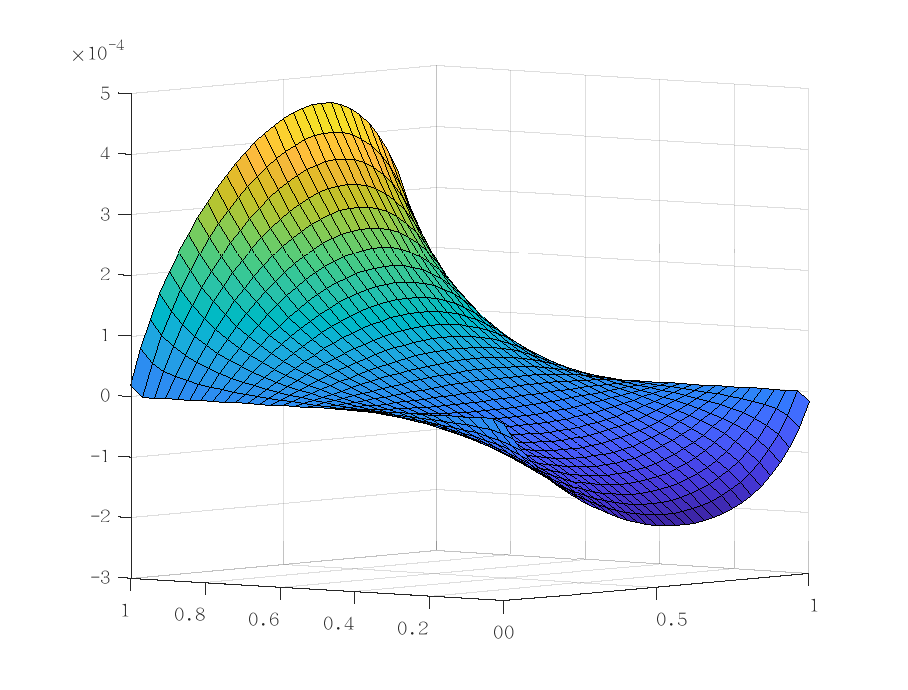
\includegraphics[width=0.8\linewidth]{figure/2-3-2.eps}
    \caption*{$n=32$}
  \end{minipage}
  \begin{minipage}[t]{0.24\linewidth}
    \centering
    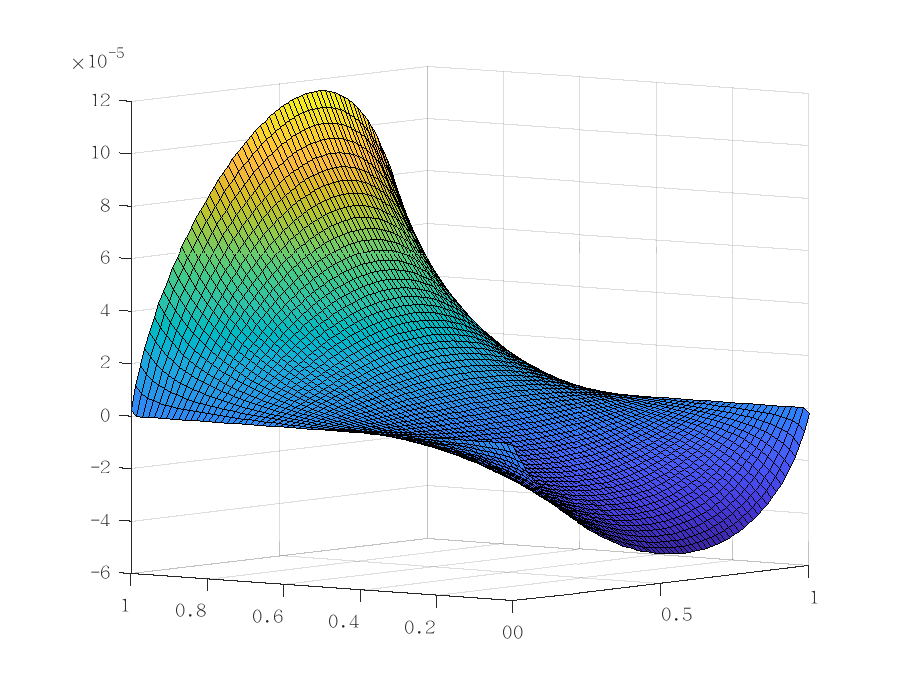
\includegraphics[width=0.8\linewidth]{figure/2-3-3.eps}
    \caption*{$n=64$}
  \end{minipage}
  \begin{minipage}[t]{0.24\linewidth}
    \centering
    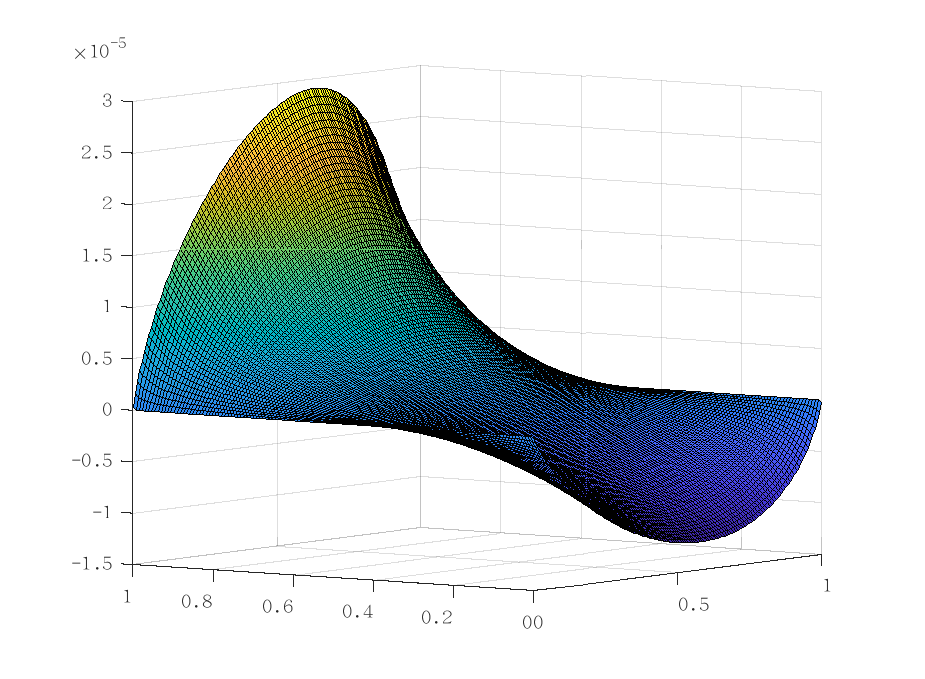
\includegraphics[width=0.8\linewidth]{figure/2-3-4.eps}
    \caption*{$n=128$}
  \end{minipage}
\end{figure}

可以看到,越靠近Dirichlet条件的边界,求解误差越小,靠近Neumann边界的求解误差会比较大。

将数值解与真实解的误差用范数估计,并根据$n=512$增加到$n=1024$时误差减小的倍数,估计各范数下的收敛阶,结果如下表。

\begin{table}[H]
  \centering
  \small
  \begin{tabular}{c|ccccccc|c}
  \textbf{$n$}        & 16                   & 32                   & 64                   & 128                  & 256                  & 512                  & 1024                  & 收敛阶 \\ \hline
  $||\cdot||_1$      & $3.91\times 10^{-4}$ & $9.65\times 10^{-5}$ & $2.40\times 10^{-5}$ & $6.00\times 10^{-6}$ & $1.50\times 10^{-6}$ & $3.75\times 10^{-7}$ & $9.37\times 10^{-8}$ & $2.001$\\
  $||\cdot||_2$      & $5.62\times 10^{-4}$ & $1.36\times 10^{-4}$ & $3.41\times 10^{-5}$ & $8.49\times 10^{-6}$ & $2.12\times 10^{-6}$ & $5.29\times 10^{-7}$ & $1.32\times 10^{-7}$ & $2.003$\\
  $||\cdot||_\infty$ & $1.79\times 10^{-3}$ & $4.56\times 10^{-4}$ & $1.15\times 10^{-4}$ & $2.90\times 10^{-5}$ & $7.29\times 10^{-6}$ & $1.82\times 10^{-6}$ & $4.57\times 10^{-7}$ & $1.994$
  \end{tabular}
\end{table}

符合二阶收敛的理论结果。

\subsection{V-Cycle 与 FMG-Cycle 的对比}

本小节中,我们用Dirichlet边值问题(4.1)做测试。限制算子采用injection,插值算子选择线性插值。

以$n=64$的网格为例,采用V-Cycle,每两步迭代的误差分布如下图。

\begin{figure}[H]
  \centering
  \begin{minipage}[t]{0.24\linewidth}
      \centering
      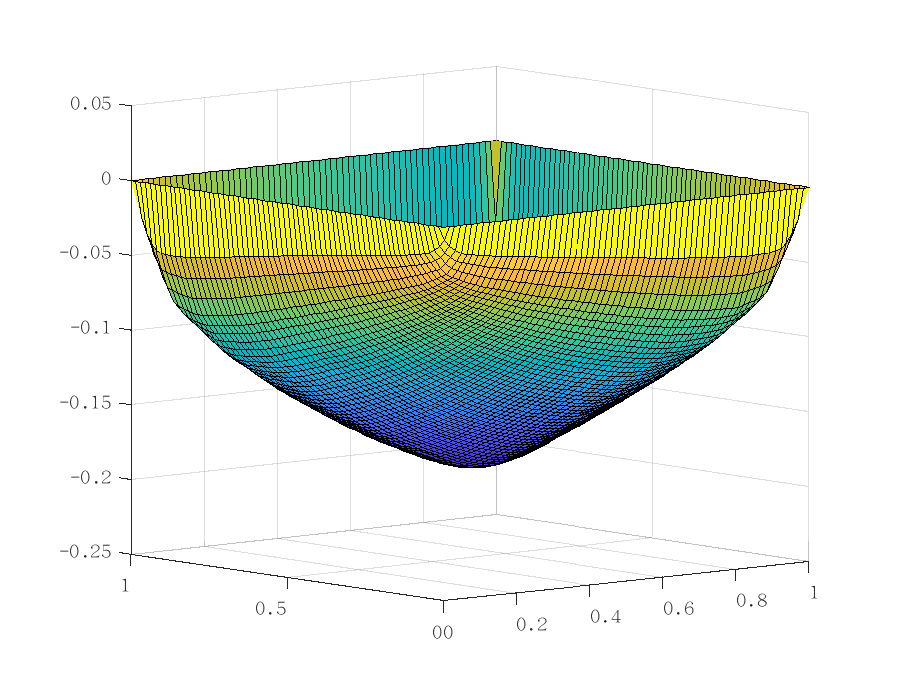
\includegraphics[width=0.8\linewidth]{figure/2-4-1.eps}
      \caption*{Iter 2}
  \end{minipage}
  \begin{minipage}[t]{0.24\linewidth}
    \centering
    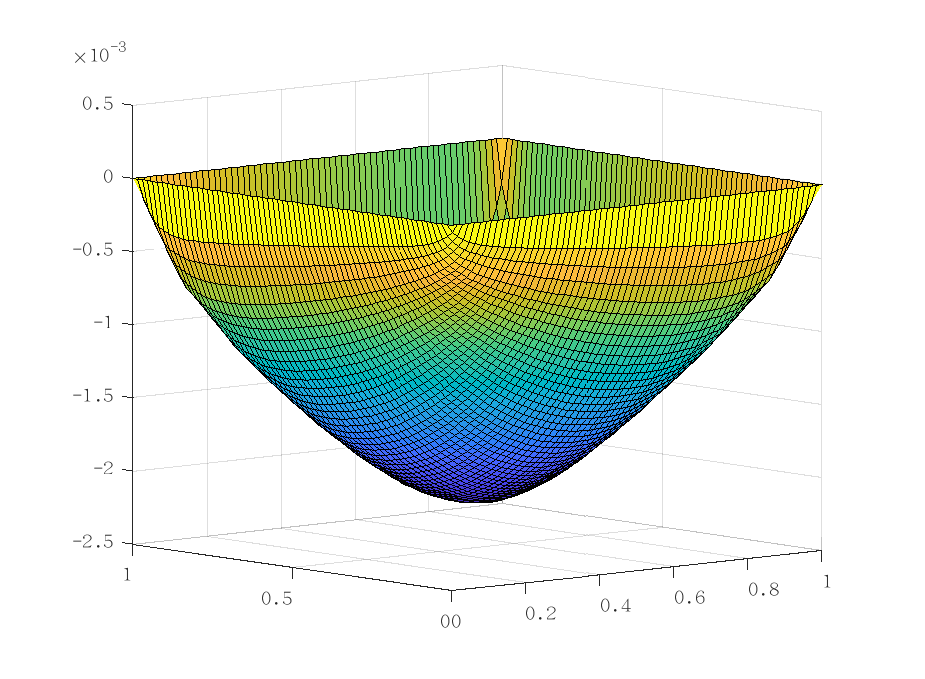
\includegraphics[width=0.8\linewidth]{figure/2-4-2.eps}
    \caption*{Iter 4}
  \end{minipage}
  \begin{minipage}[t]{0.24\linewidth}
    \centering
    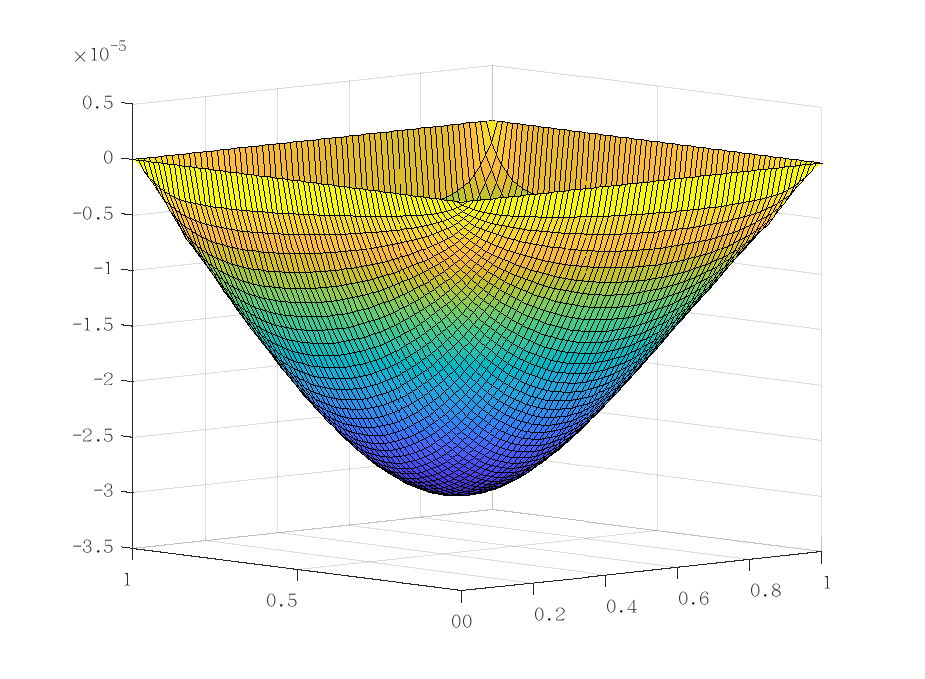
\includegraphics[width=0.8\linewidth]{figure/2-4-3.eps}
    \caption*{Iter 6}
  \end{minipage}
  \begin{minipage}[t]{0.24\linewidth}
    \centering
    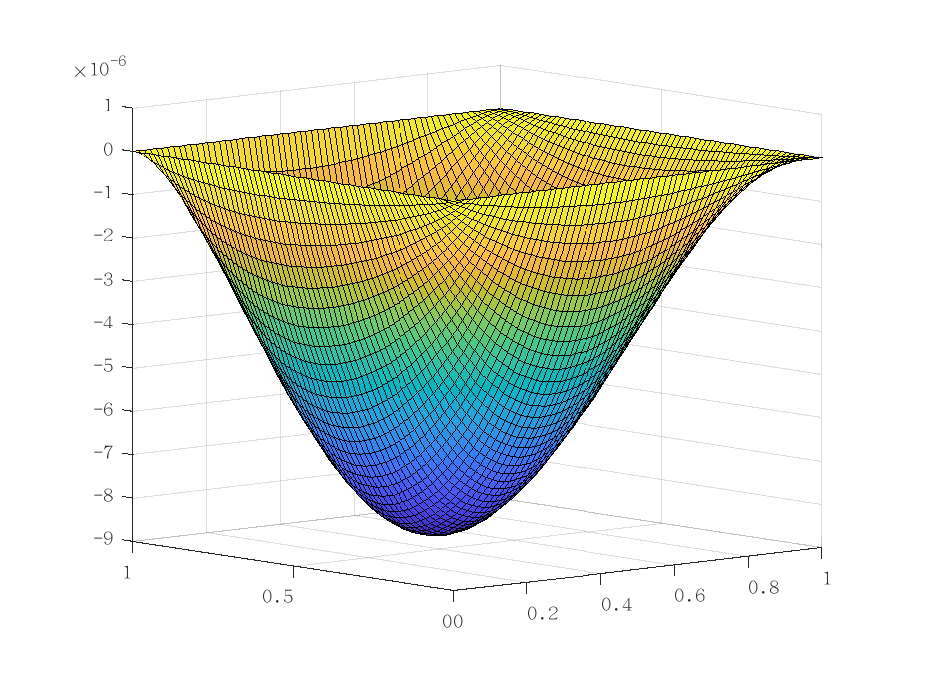
\includegraphics[width=0.8\linewidth]{figure/2-4-4.eps}
    \caption*{Iter 8}
  \end{minipage}
\end{figure}

采用FMG-Cycle,每两步迭代的误差分布如下图。

\begin{figure}[H]
  \centering
  \begin{minipage}[t]{0.24\linewidth}
      \centering
      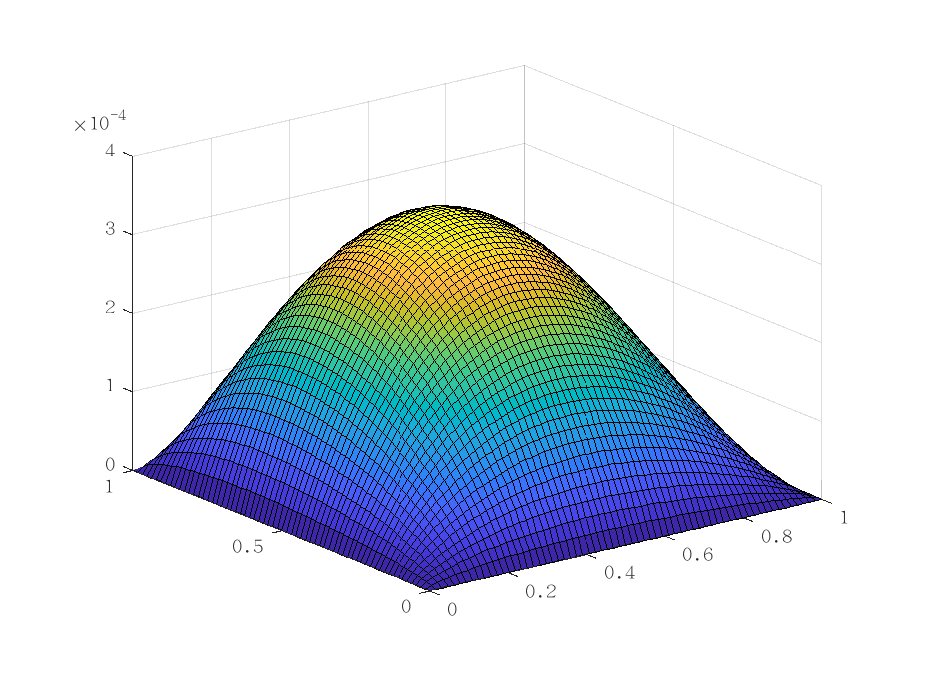
\includegraphics[width=0.8\linewidth]{figure/2-4-5.eps}
      \caption*{Iter 2}
  \end{minipage}
  \begin{minipage}[t]{0.24\linewidth}
    \centering
    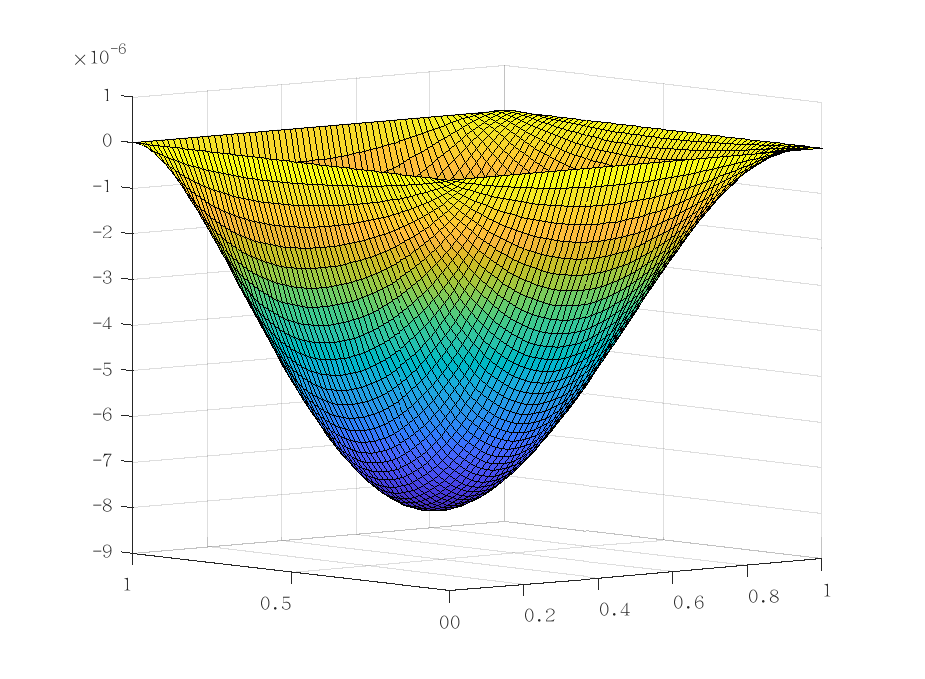
\includegraphics[width=0.8\linewidth]{figure/2-4-6.eps}
    \caption*{Iter 4}
\end{minipage}
\end{figure}

我们使用不同大小的网格,取$n=32,64,128,256,512$,用V-Cycle与FMG-Cycle分别迭代三次,误差与求解时间如下表(误差均以无穷范数计)。

\begin{table}[H]
  \centering
  \small
  \begin{tabular}{c|ccccccc}
   $\mathbf{n}$      & 32                   & 64                   & 128                  & 256                  & 512                 \\ \hline
V-Cycle   & $1.50\times 10^{-2}$ & $2.16\times 10^{-2}$ & $2.95\times 10^{-2}$ & $3.88\times 10^{-2}$ & $4.97\times 10^{-2}$  \\
FMG-Cycle   & $1.97\times 10^{-5}$ & $5.66\times 10^{-6}$ & $1.18\times 10^{-5}$ & $1.33\times 10^{-5}$ & $1.37\times 10^{-5}$  \\
离散误差$(\leq)$   & $3.45\times 10^{-5}$ & $8.62\times 10^{-6}$ & $2.16\times 10^{-6}$ & $5.39\times 10^{-7}$ & $1.35\times 10^{-7}$\\
V-Cycle 耗时$(s)$  & 0.008 & 0.017 & 0.066 & 0.211 & 0.802\\
FMG-Cycle 耗时$(s)$ & 0.011 & 0.024 & 0.077 & 0.260 & 0.905
\end{tabular}
\end{table}

可以发现,V-Cycle与FMG-Cycle迭代三次所需的时间相差无几,但是求解精度却天差地别。FMG-Cycle比V-Cycle要高效得多。

\subsection{限制算子与插值算子的选择测试}

本小节中,我们用Dirichlet边值问题(4.1)做测试。迭代方式选择V-Cycle,我们比较不同的限制算子与插值算子,设置如下四个实验组:
\begin{enumerate}[(i)]
  \item injection + 线性插值
  \item full-weighting + 线性插值
  \item injection + 二次插值
  \item full-weighting + 二次插值
\end{enumerate}

以$n=64$网格为例,采用injection + 线性插值,每步迭代的误差分布如下图。
\begin{figure}[H]
  \centering
  \begin{minipage}[t]{0.22\linewidth}
      \centering
      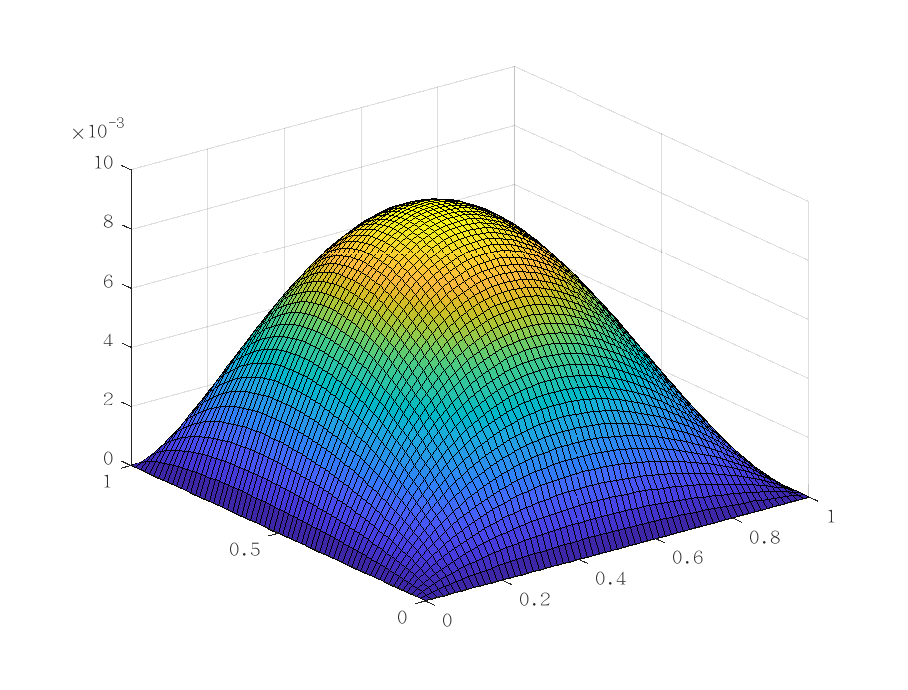
\includegraphics[width=0.84\linewidth]{figure/2-5-1.eps}
      \caption*{\small Iter 1 \\ 代数误差 $0.0087$}
  \end{minipage}
  \hspace{1em}
  \begin{minipage}[t]{0.22\linewidth}
    \centering
    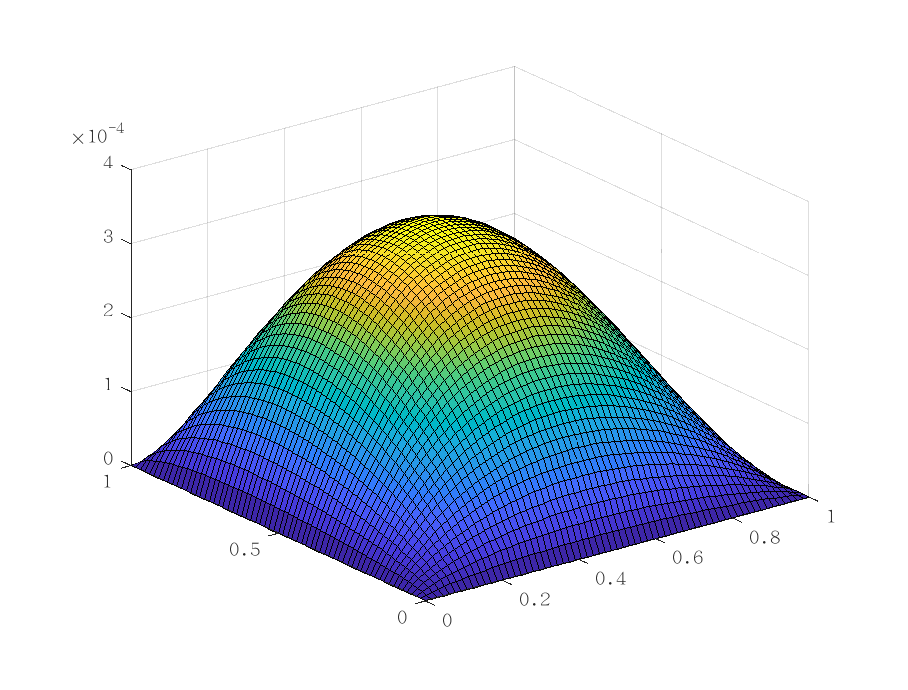
\includegraphics[width=0.84\linewidth]{figure/2-5-2.eps}
    \caption*{\small Iter 2 \\ 代数误差 $0.0003$}
  \end{minipage}
  \hspace{1em}
  \begin{minipage}[t]{0.22\linewidth}
    \centering
    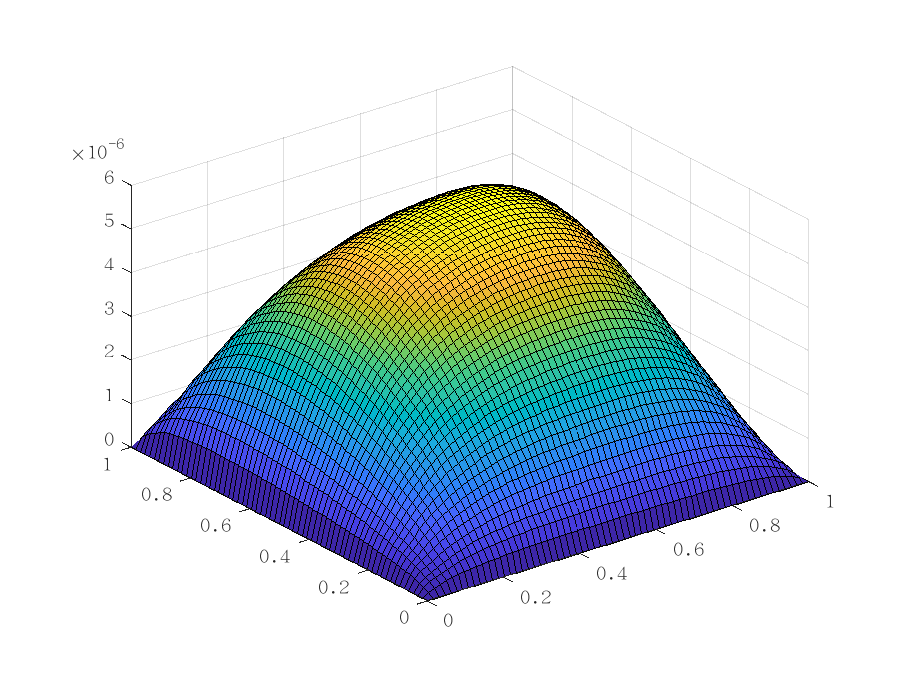
\includegraphics[width=0.84\linewidth]{figure/2-5-3.eps}
    \caption*{\small Iter 3 \\ 代数误差 $1.35\times 10^{-5}$}
  \end{minipage}
  \hspace{1em}
  \begin{minipage}[t]{0.22\linewidth}
    \centering
    \includegraphics[width=0.84\linewidth]{figure/2-5-4.eps}
    \caption*{\small Iter 4 \\ 代数误差 $5.72\times 10^{-7}$}
  \end{minipage}
\end{figure}

采用full-weighting + 线性插值,每步迭代的误差分布如下图。
\begin{figure}[H]
  \centering
  \begin{minipage}[t]{0.22\linewidth}
      \centering
      \includegraphics[width=0.84\linewidth]{figure/2-5-5.eps}
      \caption*{\small Iter 1 \\ 代数误差 $0.0002$}
  \end{minipage}
  \hspace{1em}
  \begin{minipage}[t]{0.22\linewidth}
    \centering
    \includegraphics[width=0.84\linewidth]{figure/2-5-6.eps}
    \caption*{\small Iter 2 \\ 代数误差 $3.93\times 10^{-6}$}
  \end{minipage}
  \hspace{1em}
  \begin{minipage}[t]{0.22\linewidth}
    \centering
    \includegraphics[width=0.84\linewidth]{figure/2-5-7.eps}
    \caption*{\small Iter 3 \\ 代数误差 $2.35\times 10^{-7}$}
  \end{minipage}
  \hspace{1em}
  \begin{minipage}[t]{0.22\linewidth}
    \centering
    \includegraphics[width=0.84\linewidth]{figure/2-5-8.eps}
    \caption*{\small Iter 4 \\ 代数误差 $1.61\times 10^{-8}$}
  \end{minipage}
\end{figure}

采用injection + 二次插值,每步迭代的误差分布如下图。
\begin{figure}[H]
  \centering
  \begin{minipage}[t]{0.22\linewidth}
      \centering
      \includegraphics[width=0.84\linewidth]{figure/2-5-9.eps}
      \caption*{\small Iter 1 \\ 代数误差 $3.01\times 10^{-6}$}
  \end{minipage}
  \hspace{1em}
  \begin{minipage}[t]{0.22\linewidth}
    \centering
    \includegraphics[width=0.84\linewidth]{figure/2-5-10.eps}
    \caption*{\small Iter 2 \\ 代数误差 $7.46\times 10^{-8}$}
  \end{minipage}
\end{figure}

采用full-weighting + 二次插值,每步迭代的误差分布如下图。
\begin{figure}[H]
  \centering
  \begin{minipage}[t]{0.22\linewidth}
      \centering
      \includegraphics[width=0.84\linewidth]{figure/2-5-11.eps}
      \caption*{\small Iter 1 \\ 代数误差 $2.64\times 10^{-5}$}
  \end{minipage}
  \hspace{1em}
  \begin{minipage}[t]{0.22\linewidth}
    \centering
    \includegraphics[width=0.84\linewidth]{figure/2-5-12.eps}
    \caption*{\small Iter 2 \\ 代数误差 $7.82\times 10^{-7}$}
  \end{minipage}
  \hspace{1em}
  \begin{minipage}[t]{0.22\linewidth}
    \centering
    \includegraphics[width=0.84\linewidth]{figure/2-5-13.eps}
    \caption*{\small Iter 3 \\ 代数误差 $4.33\times 10^{-8}$}
  \end{minipage}
\end{figure}

注意,上述误差分布图是真实误差的分布图,我们在图下方标注了此时的代数误差(以无穷范数计)。实际上,在代数误差下降的过程中,真实误差有时会增大,这是因为较大的代数误差有时恰好抵消了一部分离散误差,但这并不能作为最终的可信结果,我们还是应当以代数误差下降到足够小时的结果为最终结果。

我们使用不同大小的网格,取$n=2^5,2^6,...,2^{10}$,对每个实验组分别迭代求解,当代数误差达到$10^{-8}$时停止迭代,此时达到离散误差。各实验组需要的迭代次数与离散误差如下表(误差以无穷范数计)。

\begin{table}[H]
  \centering
  \small
  \begin{tabular}{c|ccccccc}
   $\mathbf{n}$       & 32                   & 64                   & 128                  & 256                  & 512      & 1024           \\ \hline
injection+线性插值   & 6 & 7 & 7 & 7 & 7 &  7 \\
full-weighting+线性插值   & 6 & 6 & 5 & 5 & 4 & 4 \\
injection+二次插值   & 5 & 4 & 3 & 3 & 3 & 3 \\
full-weighting+二次插值   & 5 & 5 & 5 & 4 & 4 & 3 \\
离散误差$(\leq)$   & $3.45\times 10^{-5}$ & $8.62\times 10^{-6}$ & $2.16\times 10^{-6}$ & $5.39\times 10^{-7}$ & $1.35\times 10^{-7}$ & $3.37\times 10^{-8}$
\end{tabular}
\end{table}

我们可以得出以下三条结论:
\begin{enumerate}
  \item 二次插值总是比线性插值好;
  \item 采用线性插值时,限制算子选择full-weighting比选择injection明显更好;
  \item 采用二次插值时,两种限制算子的效果区别不大。
\end{enumerate}

事实上,通过多次迭代,无论何种算子组合都能达到离散误差。这是因为离散误差是$O(h^2)$,而即使是最低阶的线性插值,精度也已经是$O(h^2)$,二次插值的精度则是更高阶的$O(h^3)$。

\subsection{多重网格与LU分解法的求解速度对比}

这里,我们以Dirichlet边值问题(4.1)为例,将多重网格法与Poject 01中的LU分解法进行求解速度的对比。限制算子选择Full Operator,插值算子选择二次插值,求解精度如下表(均以$\infty$范数误差计)。

\begin{table}[H]
  \centering
  \small
  \begin{tabular}{c|ccccccc}
求解方法        & 16                   & 32                   & 64                   & 128                  & 256                  & 512                  & 1024                 \\ \hline
V-Cycle        & $1.38\times 10^{-4}$ & $3.45\times 10^{-5}$ & $8.62\times 10^{-6}$ & $2.16\times 10^{-6}$ & $5.39\times 10^{-7}$ & $1.35\times 10^{-7}$ & $3.37\times 10^{-8}$  \\
FMG-Cycle      & $1.38\times 10^{-4}$ & $3.45\times 10^{-5}$ & $8.62\times 10^{-6}$ & $2.16\times 10^{-6}$ & $5.39\times 10^{-7}$ & $1.35\times 10^{-7}$ & $3.37\times 10^{-8}$  \\
LU分解         & $1.22\times 10^{-4}$ & $3.24\times 10^{-5}$ & $8.36\times 10^{-6}$ & $2.12\times 10^{-6}$ & - & - & - 
\end{tabular}
\end{table}

可以看到,LU分解的求解精度略高于多重网格,这是合理的。求解耗时如下表(单位:秒)。

\begin{table}[H]
  \centering
  \small
  \begin{tabular}{c|ccccccc|c}
求解方法        & 16                   & 32                   & 64                   & 128                  & 256                  & 512                  & 1024                & 增长阶数 \\ \hline
V-Cycle        & 0.005 & 0.011 & 0.036 & 0.105 & 0.376 & 1.440 &  6.934 & 2.268  \\
FMG-Cycle      & 0.002 & 0.015 & 0.025 & 0.090 & 0.351 & 1.182 &  3.835 & 1.698 \\
LU分解         & 0.002 & 0.022 & 0.42 & 8.168 & - & - & - & 4.281
\end{tabular}
\end{table}

根据理论结果,二维情形下,多重网格法的复杂度为$O(n^2)$,经过稀疏矩阵优化的LU分解法的复杂度为$O(n^4)$,考虑到算法具有固定的常数,上述实验结果符合理论。

\section{理论分析}

\subsection{基本表述}

在这一节中,我们以齐次Dirichlet边值问题为例给出理论分析,此时的离散方程为$A^h\mathbf{u}^h=\mathbf{f}^h$,系数矩阵$A^h\in\mathbb{R}^{n^2\times n^2}$是分块矩阵,
\begin{equation}
  A^h=\frac{1}{h^2}\begin{bmatrix}
    T & -I & \\
    -I & T & -I & \\
    & -I & T & -I &\\
    & & \ddots & \ddots & \ddots\\
    & & & -I & T
  \end{bmatrix},\qquad \text{其中}\;\;
  T=\begin{bmatrix}
    4 & -1 & \\
    -1 & 4 & -1 & \\
    & -1 & 4 & -1 &\\
    & & \ddots & \ddots & \ddots\\
    & & & -1 & 4
  \end{bmatrix}\in\mathbb{R}^{n\times n}.
\end{equation}

根据讲义Theorem 7.52,我们有:
\begin{theorem}
  式(4.4)中矩阵$A^h$的特征值与对应的特征向量为:
  \begin{equation}
    \lambda_{ij}=\lambda_i+\lambda_j,\quad \mathbf{W}_{ij}=\text{vec}(\mathbf{w}_i\mathbf{w}_j^T),\quad i,j=1,...,n-1.
  \end{equation}
  其中
  \begin{equation}
    \lambda_k=\frac{4}{h^2}\sin^2\frac{kh\pi}{2},\quad w_{k,j}=\sin(jkh\pi),\quad k,j=1,...,n-1.
  \end{equation}
\end{theorem}

\begin{lemma}
  式(4.4)中矩阵$A^h$的加权Jacobi迭代矩阵为:
  \begin{equation}
    T_\omega=(1-\omega)I+\omega D^{-1}(L+U)=I-\frac{\omega h^2}{4}A.
  \end{equation}

  $T_\omega$的特征向量与$A^h$一样,对应的特征值为:
  \begin{equation}
    \lambda_{ij}(T_\omega)=1-\frac{\omega h^2}{4}\lambda_{ij}=1-\omega\sin^2\frac{ih\pi}{2}-\omega\sin^2\frac{jh\pi}{2}.
  \end{equation}
\end{lemma}

\begin{definition}
  二维full-weighting算子由下式给出。
  \begin{equation*}
  v^{2h}_{i,j}=\frac{1}{16}(v^h_{2i-1,2j-1}+v^h_{2i-1,2j+1}+v^h_{2i+1,2j-1}+v^h_{2i+1,2j+1})
  +\frac{1}{8}(v^h_{2i,2j-1}+v^h_{2i,2j+1}+v^h_{2i-1,2j}+v^h_{2i+1,2j}) + \frac{1}{4}v^h_{2i,2j}.
  \end{equation*}
  其中$i,j=1,...,n$. 用$\mathbf{I}_h^{2h}$表示二维full-weighting算子。
\end{definition}

\begin{definition}
  二维线性插值算子$\mathbf{I}_{2h}^h=4(\mathbf{I}_h^{2h})^T.$
\end{definition}

\subsection{Two-Grid校正算子的谱半径}

我们引述讲义 Lemma 9.38 与 Lemma 9.39:
\begin{lemma}
  full-weighting算子在一对互补波上作用的结果为:
  \begin{align}
    I_h^{2h} \mathbf{w}_k^h&=c_k\mathbf{w}_k^{2h}:=\cos^2\frac{k\pi}{2n}\mathbf{w}_k^{2h},
    & I_h^{2h} \mathbf{w}_{k'}^h&=-s_k\mathbf{w}_k^{2h}:=-\sin^2\frac{k\pi}{2n}\mathbf{w}_k^{2h}
  \end{align}
  其中$k\in[1,\frac{n}{2}),k'=n-k$. 另外,$I_h^{2h}\mathbf{w}_{\frac{n}{2}}^h=\mathbf{0}$.
\end{lemma}

\begin{lemma}
  线性插值算子在波上的作用结果为:
  \begin{equation}
    I^h_{2h} \mathbf{w}_k^{2h}=c_k\mathbf{w}_k^h-s_k\mathbf{w}_{k'}^h,
  \end{equation}
  其中$k\in[1,\frac{n}{2}),k'=n-k$.
\end{lemma}

下面给出二维情形中的相应结果:
\begin{definition}
  对于$i,j\in[1,\frac{n}{2})$,记$i'=n-i,j'=n-j$,我们称$\mathbf{W}_{ij},\mathbf{W}_{ij'},\mathbf{W}_{ij'},\mathbf{W}_{i'j'}$为一组\textbf{互补波}。
\end{definition}

\begin{lemma}
  二维full-weighting算子在一组互补波上作用的结果为:
  \begin{subequations}
    \begin{align}
      \mathbf{I}_h^{2h} \mathbf{W}_{ij}^h&=c_ic_j\mathbf{W}_{ij}^{2h}, \\
      \mathbf{I}_h^{2h} \mathbf{W}_{ij'}^h&=-c_is_j\mathbf{W}_{ij}^{2h}, \\
      \mathbf{I}_h^{2h} \mathbf{W}_{i'j}^h&=-s_ic_j\mathbf{W}_{ij}^{2h}, \\
      \mathbf{I}_h^{2h} \mathbf{W}_{i'j'}^h&=s_is_j\mathbf{W}_{ij}^{2h}.
    \end{align}
  其中$i,j\in[1,\frac{n}{2}),i'=n-i,j'=n-j$. 另外
    \begin{align}
      \mathbf{I}_h^{2h}\mathbf{W}_{i\frac{n}{2}}^h&=\mathbf{0},\quad i=1,...,n-1\\
      \mathbf{I}_h^{2h}\mathbf{W}_{\frac{n}{2}j}^h&=\mathbf{0},\quad j=1,...,n-1.
    \end{align}
  \end{subequations}
\end{lemma}

\begin{proof}
  取定$i,j\in[1,\frac{n}{2})$,根据定义4.1与引理4.2,有:
  \begin{align*}
    \left(\mathbf{I}_h^{2h} \mathbf{W}_{ij}^h\right)_{kl} =& \frac{1}{4}\left(\frac{1}{4}w_{i,2k-1}+\frac{1}{2}w_{i,2k}+\frac{1}{4}w_{i,2k+1}\right)w_{j,2l-1}
    + \frac{1}{2}\left(\frac{1}{4}w_{i,2k-1}+\frac{1}{2}w_{i,2k}+\frac{1}{4}w_{i,2k+1}\right)w_{j,2l}+\\
    &\frac{1}{4}\left(\frac{1}{4}w_{i,2k-1}+\frac{1}{2}w_{i,2k}+\frac{1}{4}w_{i,2k+1}\right)w_{j,2l+1}\\
    =& \frac{1}{4}c_iw_{i,k}^{2h}w_{j,2l-1}+\frac{1}{2}c_iw_{i,k}^{2h}w_{j,2l}+\frac{1}{4}c_iw_{i,k}^{2h}w_{j,2l+1}\\
    =& c_iw_{i,k}^{2h}c_jw_{j,l}^{2h}.
  \end{align*}

  所以$\mathbf{I}_h^{2h} \mathbf{W}_{ij}^h=c_ic_j\mathbf{W}_{ij}^{2h}$. 其余结论同理可证。
\end{proof}

\begin{lemma}
  线性插值算子在波上的作用结果为:
  \begin{equation}
    I^h_{2h} \mathbf{W}_{ij}^{2h}=c_ic_j\mathbf{W}_{ij}^h-c_is_j\mathbf{W}_{ij'}^h-s_ic_j\mathbf{W}_{i'j}^h+s_is_j\mathbf{W}_{i'j'}^h,
  \end{equation}
  其中$i,j\in[1,\frac{n}{2}),i'=n-i,j'=n-j$.
\end{lemma}

\begin{proof}
  取定$i,j\in[1,\frac{n}{2})$,设$k,l\in(1,n-1)$,若$k,l$均为奇数,我们有:
  \begin{align*}
    \left(I^h_{2h} \mathbf{W}_{ij}^{2h}\right)_{kl} =& \frac{1}{4}w_{i,\frac{k-1}{2}}^{2h}w_{j,\frac{l-1}{2}}^{2h}
    +\frac{1}{4}w_{i,\frac{k-1}{2}}^{2h}w_{j,\frac{l+1}{2}}^{2h} + \frac{1}{4}w_{i,\frac{k+1}{2}}^{2h}w_{j,\frac{l-1}{2}}^{2h}
    +\frac{1}{4}w_{i,\frac{k+1}{2}+1}^{2h}w_{j,\frac{l+1}{2}}^{2h}\\
    =& \frac{1}{4}\sin(i(k-1)h\pi)\sin(j(l-1)h\pi)+\frac{1}{4}\sin(i(k-1)h\pi)\sin(j(l+1)h\pi)+\\
     &\frac{1}{4}\sin(i(k+1)h\pi)\sin(j(l-1)h\pi)+\frac{1}{4}\sin(i(k+1)h\pi)\sin(j(l+1)h\pi)\\
    =& \frac{1}{2}\sin(i(k-1)h\pi)\cos(jh\pi)w_{j,l}^h+\frac{1}{2}\sin(i(k+1)h\pi)\cos(jh\pi)w_{j,l}^h=\cos(ih\pi)\cos(jh\pi)w_{i,k}^hw_{j,l}^h.
  \end{align*}
  \begin{align*}
    &\left(c_ic_j\mathbf{W}_{ij}^h-c_is_j\mathbf{W}_{ij'}^h-s_ic_j\mathbf{W}_{i'j}^h+s_is_j\mathbf{W}_{i'j'}^h\right)_{kl}\\
    =& c_iw_{i,k}^hc_jw_{j,l}^h-c_iw_{i,k}^hs_jw_{n-j,l}^h-s_iw_{n-i,k}^hc_jw_{j,l}^h+s_iw_{n-i,k}^hs_jw_{n-j,l}^h\\
    =& \left(\cos^2\frac{ih\pi}{2}\cos^2\frac{jh\pi}{2}-\cos^2\frac{ih\pi}{2}\sin^2\frac{jh\pi}{2}-\sin^2\frac{ih\pi}{2}\cos^2\frac{jh\pi}{2}+\sin^2\frac{ih\pi}{2}\sin^2\frac{jh\pi}{2}\right)w_{i,k}^hw_{j,l}^h\\
    =& \left(\cos^2\frac{ih\pi}{2}\cos(jh\pi)-\sin^2\frac{ih\pi}{2}c_j\cos(jh\pi)\right)w_{i,k}^hw_{j,l}^h = \cos(ih\pi)\cos(jh\pi)w_{i,k}^hw_{j,l}^h.
  \end{align*}

  从而该分量得证。现在考虑$k$为偶数、$l$为奇数,我们有:
  \begin{align*}
    \left(I^h_{2h} \mathbf{W}_{ij}^{2h}\right)_{kl} =& \frac{1}{2}w_{i,\frac{k}{2}}^{2h}w_{j,\frac{l-1}{2}}^{2h}
    +\frac{1}{2}w_{i,\frac{k}{2}}^{2h}w_{j,\frac{l+1}{2}}^{2h}\\
    =& \frac{1}{2}\sin(ikh\pi)\sin(j(l-1)h\pi)+\frac{1}{2}\sin(ikh\pi)\sin(j(l+1)h\pi)\\
    =& \cos(ih\pi)w_{i,k}^hw_{j,l}^h.
  \end{align*}
  \begin{align*}
    &\left(c_ic_j\mathbf{W}_{ij}^h-c_is_j\mathbf{W}_{ij'}^h-s_ic_j\mathbf{W}_{i'j}^h+s_is_j\mathbf{W}_{i'j'}^h\right)_{kl}\\
    =& c_iw_{i,k}^hc_jw_{j,l}^h-c_iw_{i,k}^hs_jw_{n-j,l}^h-s_iw_{n-i,k}^hc_jw_{j,l}^h+s_iw_{n-i,k}^hs_jw_{n-j,l}^h\\
    =& \left(\cos^2\frac{ih\pi}{2}\cos^2\frac{jh\pi}{2}+\cos^2\frac{ih\pi}{2}\sin^2\frac{jh\pi}{2}-\sin^2\frac{ih\pi}{2}\cos^2\frac{jh\pi}{2}-\sin^2\frac{ih\pi}{2}\sin^2\frac{jh\pi}{2}\right)w_{i,k}^hw_{j,l}^h\\
    =& \left(\cos^2\frac{ih\pi}{2}-\sin^2\frac{ih\pi}{2}c_j\right)w_{i,k}^hw_{j,l}^h = \cos(ih\pi)w_{i,k}^hw_{j,l}^h.
  \end{align*}

  从而该分量得证。$k$为奇数、$l$为偶数的情况同理。此外,对于$k,l$取$1$或$n-1$时的边界情况,过于繁琐,不再赘述。综上所述(4.10)式成立。
\end{proof}

\begin{theorem}
  $\mathcal{W}_{ij}^h=\text{span}\{\mathbf{W}_{ij},\mathbf{W}_{ij'},\mathbf{W}_{ij'},\mathbf{W}_{i'j'}\}$是Two-Grid校正算子的不变子空间。
\end{theorem}

\begin{proof}
  事实上,
  \begin{equation*}
    TG=T_\omega^{\nu_2}(I-\mathbf{I}_{2h}^h(A^{2h})^{-1}\mathbf{I}_h^{2h}A^h)T_\omega^{\nu_1}.
  \end{equation*}
  根据定理4.1、引理4.1、引理4.4、引理4.5,容易验证$\mathcal{W}$是$TG$算子的不变子空间。我们经过仔细运算后发现系数过长,且不美观,故不再像讲义里那样列出。
\end{proof}

\begin{proposition}
  取$\nu_1=\nu_2=3$,有$\rho(TG)<0.1$,因此能Two-Grid校正能够快速收敛。
\end{proposition}

我们作图来验证上述命题。事实上,根据定理4.2,我们有:
\begin{equation}
  TG\begin{bmatrix}
    \mathbf{W}_{ij}^h\\
    \mathbf{W}_{ij'}^h\\
    \mathbf{W}_{i'j}^h\\
    \mathbf{W}_{i'j'}^h
  \end{bmatrix} = 
  \begin{bmatrix}
    c_{11} & c_{12} & c_{13} & c_{14}\\
    c_{21} & c_{22} & c_{23} & c_{24}\\
    c_{31} & c_{32} & c_{33} & c_{34}\\
    c_{41} & c_{42} & c_{43} & c_{44}\\
  \end{bmatrix}
  \begin{bmatrix}
    \mathbf{W}_{ij}^h\\
    \mathbf{W}_{ij'}^h\\
    \mathbf{W}_{i'j}^h\\
    \mathbf{W}_{i'j'}^h
  \end{bmatrix}
\end{equation}

因此,我们只需对每个$i,j\in[0,\frac{n}{2})$,求出相应的$C=(c_{ij})$,计算$\rho(C)$并取最大值即可得到$\rho(TG)$。我们绘制$(i,j)-\rho(C)$图,如下图所示,可以发现$\rho(TG)<0.1$。

\begin{figure}[H]
  \centering
  \begin{minipage}[t]{0.24\linewidth}
      \centering
      \includegraphics[width=0.9\linewidth]{figure/2-t-1.eps}
      \caption*{$n=8,\rho(TG)=0.0884$}
  \end{minipage}
  \hspace{1em}
  \begin{minipage}[t]{0.24\linewidth}
    \centering
    \includegraphics[width=0.9\linewidth]{figure/2-t-2.eps}
    \caption*{$n=16,\rho(TG)=0.0973$}
  \end{minipage}
  \hspace{1em}
  \begin{minipage}[t]{0.24\linewidth}
    \centering
    \includegraphics[width=0.9\linewidth]{figure/2-t-3.eps}
    \caption*{$n=32,\rho(TG)=0.0973$}
  \end{minipage}
\end{figure}

\subsection{插值与限制算子的代数性质}

\begin{lemma}
  二维线性插值算子$\mathbf{I}^h_{2h}$的列向量构成$\mathcal{R}(\mathbf{I}^h_{2h})$的一组基,因此有:
  \begin{equation}
    \text{dim} \mathcal{R}(\mathbf{I}^h_{2h}) = \left(\frac{n}{2}-1\right)^2,\quad \mathcal{N}(\mathbf{I}^h_{2h})=\left\{\mathbf{0}\right\}.
  \end{equation}
\end{lemma}

\begin{proof}
  $\mathbf{I}^h_{2h}$显然是列满秩的,因此结论显然成立。
\end{proof}

\begin{lemma}
  二维full-weighting算子的零空间与像空间的维数为:
  \begin{equation}
    \text{dim} \mathcal{R}(\mathbf{I}^{2h}_{h}) = \left(\frac{n}{2}-1\right)^2,\quad \text{dim} \mathcal{N}(\mathbf{I}^{2h}_{h})=(n-1)^2-\left(\frac{n}{2}-1\right)^2.
  \end{equation}
\end{lemma}

\begin{proof}
  $\mathbf{I}^h_{2h}$显然是行满秩的,因此必然有$\text{dim} \mathcal{R}(\mathbf{I}^{2h}_{h}) = \left(\frac{n}{2}-1\right)^2$. 根据线性映射的维数定理,即得$\text{dim} \mathcal{N}(\mathbf{I}^{2h}_{h})=(n-1)^2-\left(\frac{n}{2}-1\right)^2$.
\end{proof}

\begin{lemma}
  full-weighting算子的零空间$\mathcal{N}(\mathbf{I}^{2h}_{h})$中的一组线性独立集为:
  \begin{equation}
    \{A^h\mathbf{e}^h_{ij}:i,j\text{是奇数}\}
  \end{equation}

  其中$\mathbf{e}^h_{ij}$表示$\Omega^h$中$(i,j)$位置为$1$的单位向量。
\end{lemma}

\begin{proof}
  注意到$A^h$满秩,因此$\{A^h\mathbf{e}^h_{ij}:i,j\text{是奇数}\}$线性无关。只需证明$\mathbf{I}^{2h}_{h}A^h\mathbf{e}^h_{ij}=\mathbf{0}$,事实上:
  \begin{equation*}
    (A^h\mathbf{e}^h_{ij})_{kl}=\left\{\begin{array}{ll}
      4h^{-2}, & k=i,l=j,\\
      -h^{-2}, & k=i,l=j\pm 1\;\text{或} \;k=i\pm 1,j=l,\\
      0, & \text{其余}.
    \end{array}\right.
  \end{equation*}

  若$i,j$均为奇数,则$\mathbf{I}^{2h}_{h}A^h\mathbf{e}^h_{ij}$仅在$\left(\frac{k\pm 1}{2},\frac{l \pm 1}{2}\right)$处可能非零,但是
  \begin{equation*}
    (\mathbf{I}^{2h}_{h}A^h\mathbf{e}^h_{ij})_{\left(\frac{k\pm 1}{2},\frac{l \pm 1}{2}\right)}=\frac{1}{16}\cdot 4h^{-2} + \frac{1}{8}\cdot (-h^{-2}) + \frac{1}{8}\cdot (-h^{-2}) = 0.
  \end{equation*}

  因此$\mathbf{I}^{2h}_{h}A^h\mathbf{e}^h_{ij}=\mathbf{0}$.
\end{proof}

\begin{definition}
  对于一个正定对称矩阵$A$,我们定义:
  \begin{equation}
    \langle \mathbf{u},\mathbf{v} \rangle_A := \langle A\mathbf{u},\mathbf{v} \rangle.
  \end{equation}
  后者是通常意义下的内积。容易验证这个内积是良定义的,我们称之为“$A$内积”或“$A$能量内积”。相对应的有“$A$能量模”,如下:
  \begin{equation}
    ||\mathbf{u}||_A:=\langle \mathbf{u},\mathbf{u} \rangle_A
  \end{equation}
\end{definition}

\begin{lemma}
  在$\Omega^h$中的网格点$(i,j)$上,Laplace方程可以用九点离散表示:
  \begin{align}
    \mathcal{L} u_{ij} =& \frac{1}{3h^2}(8u_{ij}-u_{(i-1)(j-1)}-u_{(i-1)j}-u_{(i-1)(j+1)}-u_{i(j-1)}-u_{i(j+1)} \nonumber \\
    &-u_{(i+1)(j-1)}-u_{(i+1)j}-u_{(i+1)(j+1)}).
  \end{align}

  由泰勒展开容易得到:
  \begin{equation}
    \mathcal{L} u_{ij}=-\Delta u(x_i,y_j)+O(h^4).
  \end{equation}
\end{lemma}

我们设$B^h$为采用九点离散格式时的系数矩阵,有:
\begin{equation}
  B^h=\frac{1}{h^2}\begin{bmatrix}
    K & P & \\
    P & K & P & \\
    & P & K & P &\\
    & & \ddots & \ddots & \ddots\\
    & & & P & K
  \end{bmatrix}.
\end{equation}

其中
\begin{equation}
  K=\begin{bmatrix}
    8 & -1 & \\
    -1 & 8 & -1 & \\
    & -1 & 8 & -1 &\\
    & & \ddots & \ddots & \ddots\\
    & & & -1 & 8
  \end{bmatrix}\in\mathbb{R}^{n\times n}, \qquad 
  P=\begin{bmatrix}
    -1 & -1 & \\
    -1 & -1 & -1 & \\
    & -1 & -1 & -1 &\\
    & & \ddots & \ddots & \ddots\\
    & & & -1 & -1
  \end{bmatrix}\in\mathbb{R}^{n\times n}
\end{equation}

\textbf{注意:不论是在理论分析还是代码实现中,我们都不会用九点离散格式来解方程,仅以$B^h$的能量模作为分析误差的工具。}

\begin{lemma}
  线性插值算子与full-weighting算子关于$B^h$具有如下共轭性质:
  \begin{equation}
    \mathbf{I}_h^{2h}B^h\mathbf{I}_{2h}^h=B^{2h}.
  \end{equation}
\end{lemma}

\begin{proof}
  取$\Omega^{2h}$中的单位向量$\mathbf{e}^{2h}_{ij}$,只需对每个单位向量证明$\mathbf{I}_h^{2h}B^h\mathbf{I}_{2h}^h\mathbf{e}^{2h}_{ij}=B^{2h}\mathbf{e}^{2h}_{ij}$即可。我们先假定格点$(i,j)$不在边界旁边,有:
  \begin{align*}
    &(B^{2h}\mathbf{e}^{2h}_{ij})_{kl}=\left\{
    \begin{array}{ll}
      \frac{8}{3\cdot (2h)^2}=\frac{2}{3h^2}, & k=i,l=j,\\
      -\frac{1}{3\cdot (2h)^2}=-\frac{1}{12h^2}, & k=i,l=j\pm 1 \; \text{或} \; k=i\pm 1,l=j \; \text{或} \; k=i\pm 1,l=j\pm 1,\\
      0, & \text{其余}.
    \end{array}\right.\\
    &(\mathbf{I}_{2h}^h\mathbf{e}^{2h}_{ij})_{kl}=\left\{
    \begin{array}{ll}
      1, & k=2i,l=2j,\\
      \frac{1}{2}, & k=2i,l=2j\pm 1 \; \text{或} \; k=2i\pm 1,l=2j,\\
      \frac{1}{4}, & k=2i\pm 1,l=2j\pm 1,\\
      0, & \text{其余}.
    \end{array}\right.
  \end{align*}

  $B^h\mathbf{I}_{2h}^h\mathbf{e}^{2h}_{ij}=\frac{\mathbf{c}_{i,j}}{3h^2}$,其中$\mathbf{c}_{i,j}$是$\Omega^h$上的向量,值如下图所示。图的中间位置是$(2i,2j)$,右边一格是$(2i,2j+1)$,下面一格是$(2i+1,2j)$。图之外的位置为$0$。

  \begin{figure}[H]
    \centering
    \includegraphics[width=0.4\textwidth]{figure/2-t-4.png}
  \end{figure}

  从而我们有:
  \begin{align*}
    &(\mathbf{I}_{h}^{2h}B^h\mathbf{I}_{2h}^h\mathbf{e}^{2h}_{ij})_{ij}=\frac{1}{3h^2}\left(\frac{1}{4}\times 5 + \frac{1}{8}\times 1.5\times 4\right)=\frac{2}{3h^2},\\
    &(\mathbf{I}_{h}^{2h}B^h\mathbf{I}_{2h}^h\mathbf{e}^{2h}_{ij})_{(i\pm 1)j}=(\mathbf{I}_{h}^{2h}B^h\mathbf{I}_{2h}^h\mathbf{e}^{2h}_{ij})_{i(j\pm 1)} = \frac{1}{3h^2}\left(\frac{1}{4}\times (-1) + \frac{1}{8}\times (-0.75)\times 2+\frac{1}{8}\times 1.5\right)=-\frac{1}{12h^2},\\
    &(\mathbf{I}_{h}^{2h}B^h\mathbf{I}_{2h}^h\mathbf{e}^{2h}_{ij})_{(i\pm 1)(j\pm 1)}=\frac{1}{3h^2}\left(\frac{1}{4}\times (-0.25) + \frac{1}{8}\times (-0.75)\times 2\right)=-\frac{1}{12h^2},\\
    &(\mathbf{I}_{h}^{2h}B^h\mathbf{I}_{2h}^h\mathbf{e}^{2h}_{ij})_{kl}=0,\qquad k,l\text{不在上述情况中}.
  \end{align*}

  从而$\mathbf{I}_h^{2h}B^h\mathbf{I}_{2h}^h\mathbf{e}^{2h}_{ij}=B^{2h}\mathbf{e}^{2h}_{ij}$得证。对于格点$(i,j)$在边界旁边的情况,类似也可以验证,此处不再赘述。
\end{proof}

不难验证,将引理4.10中的$B^h$与$B^{2h}$换成$A^h$与$A^{2h}$,共轭性质是不成立的,这正是我们引入$B^h$的理由。

\subsection{FMG-Cycle的误差分析}

\begin{definition}
  我们知道,微分方程数值解在格点$(x_i,y_j)$处的误差为
  \begin{equation*}
    E_{ij}^h:=v^h_{ij}-u(x_i,y_j)=v_{ij}^h-u_{ij}^h+u_{ij}^h-u(x_i,y_j).
  \end{equation*}
  其中$v_{ij}^h-u_{ij}^h$是多重网格法解方程带来的误差,我们称之为“代数误差”;$u_{ij}^h-u(x_i,y_j)$是微分方程离散化带来的误差,我们称之为“离散误差”。
\end{definition}

\begin{lemma}
二维线性插值带来的误差在$B^h$能量模下,具有如下等式。
\begin{equation}
  ||\mathbf{I}_{2h}^h\mathbf{v}^{2h}-\mathbf{I}_{2h}^h\mathbf{u}^{2h}||_{B^h}=2||\mathbf{v}^{2h}-\mathbf{u}^{2h}||_{B^{2h}}.
\end{equation}
\end{lemma}

\begin{proof}
  根据定义4.2、定义4.4与引理4.10,我们有
  \begin{align*}
    & ||\mathbf{v}^{2h}-\mathbf{u}^{2h}||^2_{B^{2h}} = \langle B^{2h}(\mathbf{v}^{2h}-\mathbf{u}^{2h}), \mathbf{v}^{2h}-\mathbf{u}^{2h} \rangle = \langle \mathbf{I}_h^{2h}B^{h}\mathbf{I}_{2h}^h(\mathbf{v}^{2h}-\mathbf{u}^{2h}), \mathbf{v}^{2h}-\mathbf{u}^{2h} \rangle\\
    =& \frac{1}{4}\langle B^{h}\mathbf{I}_{2h}^h(\mathbf{v}^{2h}-\mathbf{u}^{2h}), \mathbf{I}_{2h}^{h}(\mathbf{v}^{2h}-\mathbf{u}^{2h}) \rangle =\frac{1}{4}||\mathbf{I}_{2h}^h(\mathbf{v}^{2h}-\mathbf{u}^{2h})||^2_{B^h}
  \end{align*}

  即得证。
\end{proof}

\begin{lemma}
  假设存在常数$K>0$,使得
  \begin{equation}
    ||\mathbf{I}_{2h}^h \mathbf{u}^{2h}-\mathbf{u}^{h}||_{B^h}\leq Kh^2.
  \end{equation}

  那么一次FMG-Cycle的代数误差有如下估计:
  \begin{equation}
    ||\mathbf{e}^h||_{B^h}\leq Kh^2.
  \end{equation}
\end{lemma}

\begin{proof}
  用数学归纳法证明。在最粗的网格上,FMG是精确求解的,因此误差估计成立。现在假设在$\Omega^{2h}$上,有误差估计
  \begin{equation*}
    ||\mathbf{e}^{2h}||_{B^{2h}}\leq K(2h)^2.
  \end{equation*}

  考虑初始代数误差$\mathbf{e}_0^h=\mathbf{I}_{2h}^h\mathbf{v}^{2h}-\mathbf{u}^h$,根据条件以及引理4.11,有如下估计:
  \begin{align*}
    ||\mathbf{e}_0^h||_{B^h}&=||\mathbf{I}_{2h}^h\mathbf{v}^{2h}-\mathbf{I}_{2h}^h\mathbf{u}^{2h}||_{B^h}+||\mathbf{I}_{2h}^h\mathbf{u}^{2h}-\mathbf{u}^h||_{B^h}\\
    &=2||\mathbf{v}^{2h}-\mathbf{u}^{2h}||_{B^h}+||\mathbf{I}_{2h}^h\mathbf{u}^{2h}-\mathbf{u}^h||_{B^h}\\
    &\leq 2K(2h)^2+Kh^2=9Kh^2.
  \end{align*}

  在命题4.1中,我们验证了$\rho(TG)<0.1$,因此经过一次$V(3,3)$-Cycle,代数误差$||\mathbf{e}^h||_{B^h}$可以降至$Kh^2$,从而归纳得证。
\end{proof}

\begin{theorem}
  对于二维齐次Dirichlet边值问题,只需要一次FMG-Cycle迭代,就能够达到$O(h^2)$精度,计算耗时$O(n^2)$。
\end{theorem}

\begin{proof}
  考虑二范数 $||\cdot||_2$,注意到 $\lambda_{\min}(B^h)=O(1)\approx 60$,再由引理4.12,存在$C,K>0$,使得:
  \begin{equation*}
    ||\mathbf{u}^h-\mathbf{v}^h||_2\leq \lambda^{-1}_{\min}(B^h)||\mathbf{u}^h-\mathbf{v}^h||_{B^h}\leq \lambda^{-1}_{\min}(B^h)CKh^2.
  \end{equation*}

  又由泰勒展开知道离散误差$||\mathbf{u}^h-\mathbf{u}||_2=O(h^2)$,因此:
  \begin{equation*}
    ||\mathbf{E}^h||_2\leq ||\mathbf{u}^h-\mathbf{u}||_2+||\mathbf{u}^h-\mathbf{v}^h||_2=O(h^2).
  \end{equation*}
\end{proof}

\newpage

\chapter{二维不规则区域中的BVP}

在本节中,我们求解区域$\Omega=\{(x,y):x\in(0,1),y\in(D(x),1)\}$中的Poisson方程,其中$D(x)=\frac{1}{16}\sin(\pi x).$

\section{设计要点}

\subsection{扭曲网格简介}

对于不规则区域的方程求解,我们想出了三种思路:

\begin{itemize}
  \item 添加不规则点,增加额外的方程,与Project 01类似。这个方法的问题在于添加的方程过于不规则,严重破坏矩阵的性质,导致Jacobi迭代发散。
  \item 坐标变换。将不规则区域的方程变换到规则区域求解,再将结果映射回不规则区域。这是一个建设性的想法,但是我们没有选择它。
  \item 扭曲网格。将整个网格沿着不规则区域的形状扭曲,如下图所示,这就是我们的方法。
\end{itemize}

\begin{figure}[H]
  \centering
  \includegraphics[width=0.4\textwidth]{figure/3-1.eps}
  \caption{扭曲网格示意图}
\end{figure}

在宽度为$h=\frac{1}{n}$的扭曲网格中,网格点$G^h(i,j)$的实际坐标为:
\begin{equation*}
  G^h(i,j)=(ih,\;D(ih)+jh(1-D(ih)))
\end{equation*}

\subsection{扭曲网格中的Laplace方程}

在规则网格中,我们可以通过上下左右四个点,给出Laplace方程的离散格式。在扭曲网格中,由于左右两个格点不在同一水平线上,因此二阶泰勒展开会存在$xy$交叉项。为将其消去,我们需要一个额外的的点。具体而言,记
\begin{align*}
  P_0&=G^h(i,j) & P_1&=G^h(i,j+1) & P_2&=G^h(i,j-1)\\
  P_3&=G^h(i+1,j) & P_4&=G^h(i-1,j) & P_5&=G^h(i+1,j+1)
\end{align*}

对于$i=0,...,5$,我们记$P_i=(x_i,y_i)$,将$P_i$处的点值在$P_0$处做二阶Taylor展开:
\begin{align*}
  u(P_i)&=u(P_0)+(x_i-x_0)\frac{\partial u}{\partial x}(P_0)+(y_i-y_0)\frac{\partial u}{\partial y}(P_0)
  +\frac{1}{2}(x_i-x_0)^2\frac{\partial^2 u}{\partial x^2}(P_0) \\
  & +\frac{1}{2}(y_i-y_0)^2\frac{\partial^2 u}{\partial y^2}(P_0)
  +(x_i-x_0)(y_i-y_0)\frac{\partial^2 u}{\partial x \partial y}(P_0)+O(h^3).
\end{align*}

列出六元一次方程组,解出系数$A_0,...,A_6$,使得
\begin{equation*}
  \sum_{i=0}^6 A_iu(P_i)=-\Delta u(P_0)+O(h)
\end{equation*}

这样列出的方程不够美观。因此我们更换$P_5$的选取,分别选择$G^h(i+1,j-1),G^h(i-1,j+1),G^h(i-1,j-1)$重复上述过程,一共求得四组系数,将各组系数在对应点处相加,再乘以$\frac{1}{4}$,即可得到更加对称的离散化Laplace方程。特别地,在靠近边界的格点处,上述过程会存在越界风险,因此需要视格点位置做特殊处理。

以$n=32,i=4,j=6$为例,通过上述方法求得的各点系数如下图所示,可以看到大体上与规则网格类似。

\begin{figure}[H]
  \centering
  \includegraphics[width=0.4\textwidth]{figure/3-2.eps}
\end{figure}

\subsection{扭曲网格中的Neumann边值条件方程}

\subsubsection{$x=0$与$x=1$边界}

这里仅以$x=0$边界为例,$x=1$边界是完全对称的。在规则网格中,对于$(0,jh)$处的法向导数,只需要$U_{0,j},U_{1,j},U_{2,j}$三个点值,即可得到二阶估计。但是在扭曲网格中,这三点之间存在$y$方向的偏移,因此二阶Taylor展式中存在$y,y^2,xy$项,这就需要额外的三个点来消除。与Laplace方程的方法完全类似,选取六个点:
\begin{align*}
  P_0&=G^h(0,j) & P_1&=G^h(1,j) & P_2&=G^h(2,j)\\
  P_3&=G^h(0,j-1) & P_4&=G^h(0,j+1) & P_5&=G^h(1,j+1).
\end{align*}

对于$i=0,...,5$,我们记$P_i=(x_i,y_i)$,将$P_i$处的点值在$P_0$处做二阶Taylor展开:
\begin{align*}
  u(P_i)&=u(P_0)+(x_i-x_0)\frac{\partial u}{\partial x}(P_0)+(y_i-y_0)\frac{\partial u}{\partial y}(P_0)
  +\frac{1}{2}(x_i-x_0)^2\frac{\partial^2 u}{\partial x^2}(P_0) \\
  & +\frac{1}{2}(y_i-y_0)^2\frac{\partial^2 u}{\partial y^2}(P_0)
  +(x_i-x_0)(y_i-y_0)\frac{\partial^2 u}{\partial x \partial y}(P_0)+O(h^3).
\end{align*}

列出六元一次方程组,解出系数$A_0,...,A_6$,使得
\begin{equation*}
  \sum_{i=0}^6 A_iu(P_i)=-u_x(P_0)+O(h^2)
\end{equation*}

为使方程更加对称,我们更换$P_5$的选取,取$P_5=G^h(1,j-1)$,重复上述过程,得到另一组系数,将各组系数在对应点处相加,再乘以$\frac{1}{2}$,即可得到更加对称的Neumann边界条件方程。特别地,在靠近上下边界的格点处,上述过程会存在越界风险,因此需要视格点位置做特殊处理。

以$n=32,j=6$为例,通过上述方法求得的各点系数如下图所示,可以看到大体上与规则网格类似。

\begin{figure}[H]
  \centering
  \includegraphics[width=0.35\textwidth]{figure/3-3.eps}
\end{figure}

\subsubsection{$y=1$边界}

我们记$h_i=\frac{1}{n}(1-D(ih))$,表示扭曲网格在$x=ih$列中的纵向间隔,那么根据二阶Taylor展开,有:
\begin{equation*}
  \frac{\partial u}{\partial y}(ih,1) = \frac{1}{2h_i}(3U_{i,n}-4U_{i,n-1}+U_{i,n-2})+O(h_i^2).
\end{equation*}

\subsubsection{下边界}

在$x=ih$处,下边界的法向量$\mathbf{n}$为:
\begin{equation}
  \mathbf{n}=\frac{1}{\sqrt{\frac{\pi^2}{256}\cos^2(\pi x)+1}}\left(\frac{\pi}{16}\cos(\pi x),1\right)
\end{equation}

仍利用二阶Taylor展开,选取六个点:
\begin{align*}
  P_0&=G^h(i,0) & P_1&=G^h(i,1) & P_2&=G^h(i,2)\\
  P_3&=G^h(i-1,0) & P_4&=G^h(i+1,0) & P_5&=G^h(i-1,1).
\end{align*}

对于$i=0,...,5$,我们记$P_i=(x_i,y_i)$,将$P_i$处的点值在$P_0$处做二阶Taylor展开:
\begin{align*}
  u(P_i)&=u(P_0)+(x_i-x_0)\frac{\partial u}{\partial x}(P_0)+(y_i-y_0)\frac{\partial u}{\partial y}(P_0)
  +\frac{1}{2}(x_i-x_0)^2\frac{\partial^2 u}{\partial x^2}(P_0) \\
  & +\frac{1}{2}(y_i-y_0)^2\frac{\partial^2 u}{\partial y^2}(P_0)
  +(x_i-x_0)(y_i-y_0)\frac{\partial^2 u}{\partial x \partial y}(P_0)+O(h^3).
\end{align*}

列出六元一次方程组,解出系数$A_0,...,A_5$,使得
\begin{equation*}
  \sum_{i=0}^5 A_iu(P_i)=\frac{\partial u}{\partial \mathbf{n}}(P_0)+O(h^2)
\end{equation*}

为使方程更加对称,我们更换$P_5$的选取,取$P_5=G^h(i+1,1)$,重复上述过程,得到另一组系数,将各组系数在对应点处相加,再乘以$\frac{1}{2}$,即可得到更加对称的Neumann边界条件方程。特别地,在靠近上下边界的格点处,上述过程会存在越界风险,因此需要视格点位置做特殊处理。

以$n=32,i=4$为例,通过上述方法求得的各点系数如下图所示,可以看到大体上与规则网格相近。

\begin{figure}[H]
  \centering
  \includegraphics[width=0.3\textwidth]{figure/3-4.eps}
\end{figure}

\subsection{扭曲网格中的线性插值}

对于一个细网格上的点,它的位置可能有四种情况:在粗网格点上、在粗网格的某条竖直线上、在粗网格的某条水平线上、不在粗网格线上。对于前两种情况,我们的处理方式与规则网格一样。对于第三种情况,因为扭曲网格的格点与左右两格点并不在同一直线上,因此需要引入第三点做线性插值。

我们只介绍不在粗网格线上点如何插值。考虑点$P_0=G^h(2i+1,2j+1)$,选取粗网格上三个点:
\begin{align*}
  P_1&=G^{2h}(i,j) & P_1&=G^{2h}(i,j+1) & P_2&=G^{2h}(i+1,j)
\end{align*}

对于$i=0,...,3$,我们记$P_i=(x_i,y_i)$,将$P_i$处的点值在$P_0$处做一阶Taylor展开:
\begin{align*}
  u(P_i)&=u(P_0)+(x_i-x_0)\frac{\partial u}{\partial x}(P_0)+(y_i-y_0)\frac{\partial u}{\partial y}(P_0)
  +\frac{1}{2}(x_i-x_0)^2\frac{\partial^2 u}{\partial x^2}(P_0) + O(h^2).
\end{align*}

列出三元一次方程组,解出系数$A_1,...,A_3$,使得
\begin{equation*}
  \sum_{i=1}^3 A_iu(P_i)=u(P_0)+O(h^2)
\end{equation*}

为了使插值系数更加对称,我们重新选取$P_1,P_2,P_3$,每次在$P_0$周围的四个粗网格点上取三个点做上述过程,取遍所有可能,一共四次。将每次得到的系数在各点处相加并乘$\frac{1}{4}$,即可得到更加对称的线性插值方程。

以$n=32,i=5,j=7$为例,各点插值系数如下图所示,与规则网格的插值系数只相差大约$0.001$.
\begin{figure}[H]
  \centering
  \includegraphics[width=0.35\textwidth]{figure/3-5.eps}
\end{figure}

在最早先版本的代码中,我们实现了不规则网格的线性插值(见gitee用户Wenchong Huang在4月14日凌晨0点14分的commit),当时我们并没有发现插值系数与规则网格如此相近。意识到这个情况后,在最终版本的代码中,出于计算性能考虑,我们选择直接使用规则网格的线性插值作为近似。

\subsection{扭曲网格中的二次插值}

这里以$P_0=G^{h}(2i+1,2j+1)$的二次插值为例讲解思路,不在赘述网格线上的点与边界附近点的特殊讨论。

选取粗网格上六个点:
\begin{align*}
  P_1&=G^{2h}(i,j) & P_2&=G^{2h}(i,j+1) & P_3&=G^{2h}(i+1,j)\\
  P_4&=G^{2h}(i+1,j+1) & P_5&=G^{2h}(i,j+2) & P_6&=G^{2h}(i+2,j)
\end{align*}

对于$i=0,...,6$,我们记$P_i=(x_i,y_i)$,将$P_i$处的点值在$P_0$处做二阶Taylor展开:
\begin{align*}
  u(P_i)&=u(P_0)+(x_i-x_0)\frac{\partial u}{\partial x}(P_0)+(y_i-y_0)\frac{\partial u}{\partial y}(P_0)
  +\frac{1}{2}(x_i-x_0)^2\frac{\partial^2 u}{\partial x^2}(P_0) \\
  & +\frac{1}{2}(y_i-y_0)^2\frac{\partial^2 u}{\partial y^2}(P_0)
  +(x_i-x_0)(y_i-y_0)\frac{\partial^2 u}{\partial x \partial y}(P_0)+O(h^3).
\end{align*}

列出六元一次方程组,解出系数$A_1,...,A_6$,使得
\begin{equation*}
  \sum_{i=1}^6 A_iu(P_i)=u(P_0)+O(h^3)
\end{equation*}

为了使插值系数更加对称,我们重新选取$P_5,P_6$:
\begin{enumerate}
  \item $P_5=G^{2h}(i+2,j+1),\;P_6=G^{2h}(i,j-1)$;
  \item $P_5=G^{2h}(i+1,j-1),\;P_6=G^{2h}(i-1,j+1)$;
  \item $P_5=G^{2h}(i-1,j),\;P_6=G^{2h}(i+1,j+2)$.
\end{enumerate}

重新选取$P_5,P_6$后重复上述过程。一共四次。将每次得到的系数在各点处相加并乘$\frac{1}{4}$,即可得到更加对称的二次插值方程。

这里不再举例展示各点插值系数,经过实际测试,与规则网格的插值系数只相差大约$0.001$。在最早先版本的代码中,我们实现了不规则网格的二次插值(见gitee用户Wenchong Huang在4月14日凌晨0点14分的commit),当时我们并没有发现插值系数与规则网格如此相近。意识到这个情况后,在最终版本的代码中,出于计算性能考虑,我们选择直接使用规则网格的二次插值作为近似。

\section{数值实验}

\subsection{Dirichlet边值问题的求解、误差分析、收敛性分析}

考虑由精确解$u(x,y)=e^{\sin x+y}$导出的Dirichlet边值问题
\begin{equation}
  \left\{
    \begin{array}{l}
      -\Delta u = -(1-\sin x+\cos^2 x)e^{\sin x + y},\quad x\in\Omega \\
      u|_{\partial \Omega}=e^{\sin x + y}
    \end{array}
  \right. .
\end{equation}

我们用$n=16,32,64,128,256,512,1024$的网格测试,使用V-Cycle,限制算子选择Full Operator,插值算子选择线性插值。当$n=16,32,64,128$时,误差分布如下图所示。
\begin{figure}[H]
  \centering
  \begin{minipage}[t]{0.24\linewidth}
      \centering
      \includegraphics[width=0.95\linewidth]{figure/3-1-1.eps}
      \caption*{$n=16$}
  \end{minipage}
  \begin{minipage}[t]{0.24\linewidth}
    \centering
    \includegraphics[width=0.95\linewidth]{figure/3-1-2.eps}
    \caption*{$n=32$}
  \end{minipage}
  \begin{minipage}[t]{0.24\linewidth}
    \centering
    \includegraphics[width=0.95\linewidth]{figure/3-1-3.eps}
    \caption*{$n=64$}
  \end{minipage}
  \begin{minipage}[t]{0.24\linewidth}
    \centering
    \includegraphics[width=0.95\linewidth]{figure/3-1-4.eps}
    \caption*{$n=128$}
  \end{minipage}
\end{figure}

可以看到,在Dirichlet条件下,格点越靠近边界,最终的计算误差越小。将数值解与真实解的误差用范数估计,并根据$n=512$增加到$n=1024$时误差减小的倍数,估计各范数下的收敛阶,结果如下表。

\begin{table}[H]
  \centering
  \small
  \begin{tabular}{c|ccccccc|c}
  \textbf{$n$}        & 16                   & 32                   & 64                   & 128                  & 256                  & 512                  & 1024                  & 收敛阶 \\ \hline
  $||\cdot||_1$      & $4.83\times 10^{-5}$ & $1.29\times 10^{-5}$ & $3.35\times 10^{-6}$ & $8.72\times 10^{-7}$ & $2.40\times 10^{-7}$ & $5.42\times 10^{-8}$ & $1.41\times 10^{-8}$ & $1.944$\\
  $||\cdot||_2$      & $6.55\times 10^{-5}$ & $1.69\times 10^{-5}$ & $4.31\times 10^{-6}$ & $1.11\times 10^{-6}$ & $2.99\times 10^{-7}$ & $6.86\times 10^{-8}$ & $1.77\times 10^{-8}$ & $1.952$\\
  $||\cdot||_\infty$ & $1.39\times 10^{-4}$ & $3.49\times 10^{-5}$ & $8.77\times 10^{-6}$ & $2.23\times 10^{-6}$ & $5.96\times 10^{-7}$ & $1.38\times 10^{-7}$ & $3.54\times 10^{-8}$ & $1.958$
  \end{tabular}
\end{table}

大致呈二阶收敛。

\subsection{Neumann边值问题的求解、误差分析、收敛性分析}

考虑由精确解$u(x,y)=e^{\sin x+y}$导出的Neumann边值问题
\begin{equation}
  \left\{
    \begin{array}{l}
      -\Delta u = -(1-\sin x+\cos^2 x)e^{\sin x + y},\quad x\in\Omega, \\
      \frac{\partial u}{\partial \mathbf{n}}|_{x=0}=-e^{y},\\
      \frac{\partial u}{\partial \mathbf{n}}|_{x=1}=\cos 1 \cdot e^{\sin 1 + y},\\
      \frac{\partial u}{\partial \mathbf{n}}|_{y=D(x)}=\cos x\cdot e^{\sin x + y} \cdot \mathbf{n}_x + e^{\sin x + y} \cdot \mathbf{n}_y,\\
      \frac{\partial u}{\partial \mathbf{n}}|_{y=1}=e^{\sin x+1}
    \end{array}
  \right. .
\end{equation}

其中$\mathbf{n}$的表达式见5.1.3小节中的式(5.1)。

我们用$n=16,32,64,128,256,512,1024$的网格测试,使用V-Cycle,限制算子选择Full Operator,插值算子选择二次插值。当$n=16,32,64,128$时,误差分布如下图所示。
\begin{figure}[H]
  \centering
  \begin{minipage}[t]{0.24\linewidth}
      \centering
      \includegraphics[width=0.95\linewidth]{figure/3-2-1.eps}
      \caption*{$n=16$}
  \end{minipage}
  \begin{minipage}[t]{0.24\linewidth}
    \centering
    \includegraphics[width=0.95\linewidth]{figure/3-2-2.eps}
    \caption*{$n=32$}
  \end{minipage}
  \begin{minipage}[t]{0.24\linewidth}
    \centering
    \includegraphics[width=0.95\linewidth]{figure/3-2-3.eps}
    \caption*{$n=64$}
  \end{minipage}
  \begin{minipage}[t]{0.24\linewidth}
    \centering
    \includegraphics[width=0.95\linewidth]{figure/3-2-4.eps}
    \caption*{$n=128$}
  \end{minipage}
\end{figure}

将数值解与真实解的误差用范数估计,并根据$n=512$增加到$n=1024$时误差减小的倍数,估计各范数下的收敛阶,结果如下表。

\begin{table}[H]
  \centering
  \small
  \begin{tabular}{c|ccccccc|c}
  \textbf{$n$}        & 16                   & 32                   & 64                   & 128                  & 256                  & 512                  & 1024                  & 收敛阶 \\ \hline
  $||\cdot||_1$      & $1.23\times 10^{-3}$ & $2.92\times 10^{-4}$ & $7.11\times 10^{-5}$ & $1.76\times 10^{-5}$ & $4.36\times 10^{-6}$ & $1.09\times 10^{-6}$ & $2.72\times 10^{-7}$ & $2.001$\\
  $||\cdot||_2$      & $1.49\times 10^{-3}$ & $3.55\times 10^{-4}$ & $8.65\times 10^{-5}$ & $2.14\times 10^{-5}$ & $5.31\times 10^{-6}$ & $1.32\times 10^{-6}$ & $3.31\times 10^{-7}$ & $2.001$\\
  $||\cdot||_\infty$ & $3.21\times 10^{-3}$ & $7.87\times 10^{-4}$ & $1.95\times 10^{-4}$ & $4.84\times 10^{-5}$ & $1.21\times 10^{-5}$ & $3.02\times 10^{-6}$ & $7.54\times 10^{-7}$ & $2.000$
  \end{tabular}
\end{table}

大致呈二阶收敛。

\subsection{混合边值问题的求解、误差分析、收敛性分析}

考虑由精确解$u(x,y)=e^{\sin x+y}$导出的混合边值问题
\begin{equation}
  \left\{
    \begin{array}{l}
      -\Delta u = -(1-\sin x+\cos^2 x)e^{\sin x + y},\quad x\in\Omega, \\
      u|_{x=0}=e^{y},\\
      u|_{x=1}=e^{y+\sin 1},\\
      \frac{\partial u}{\partial \mathbf{n}}|_{y=D(x)}=\cos x\cdot e^{\sin x + y} \cdot \mathbf{n}_x + e^{\sin x + y} \cdot \mathbf{n}_y,\\
      \frac{\partial u}{\partial \mathbf{n}}|_{y=1}=e^{\sin x+1}
    \end{array}
  \right. .
\end{equation}

其中$\mathbf{n}$的表达式见5.1.3小节中的式(5.1)。

我们用$n=16,32,64,128,256,512,1024$的网格测试,使用FMG-Cycle,限制算子选择Injection,插值算子选择线性插值。当$n=16,32,64,128$时,误差分布如下图所示。

\begin{figure}[H]
  \centering
  \begin{minipage}[t]{0.24\linewidth}
      \centering
      \includegraphics[width=0.95\linewidth]{figure/3-3-1.eps}
      \caption*{$n=16$}
  \end{minipage}
  \begin{minipage}[t]{0.24\linewidth}
    \centering
    \includegraphics[width=0.95\linewidth]{figure/3-3-2.eps}
    \caption*{$n=32$}
  \end{minipage}
  \begin{minipage}[t]{0.24\linewidth}
    \centering
    \includegraphics[width=0.95\linewidth]{figure/3-3-3.eps}
    \caption*{$n=64$}
  \end{minipage}
  \begin{minipage}[t]{0.24\linewidth}
    \centering
    \includegraphics[width=0.95\linewidth]{figure/3-3-4.eps}
    \caption*{$n=128$}
  \end{minipage}
\end{figure}

可以看到,越靠近Dirichlet条件的边界,求解误差越小,靠近Neumann边界的求解误差会比较大。且误差分布图的形状与4.2.3节中规则网格的结果大致相似。

将数值解与真实解的误差用范数估计,并根据$n=512$增加到$n=1024$时误差减小的倍数,估计各范数下的收敛阶,结果如下表。

\begin{table}[H]
  \centering
  \small
  \begin{tabular}{c|ccccccc|c}
  \textbf{$n$}        & 16                   & 32                   & 64                   & 128                  & 256                  & 512                  & 1024                  & 收敛阶 \\ \hline
  $||\cdot||_1$      & $3.54\times 10^{-4}$ & $8.74\times 10^{-5}$ & $2.18\times 10^{-5}$ & $5.44\times 10^{-6}$ & $1.36\times 10^{-6}$ & $3.41\times 10^{-7}$ & $8.59\times 10^{-8}$ & $1.990$\\
  $||\cdot||_2$      & $5.05\times 10^{-4}$ & $1.23\times 10^{-4}$ & $3.06\times 10^{-5}$ & $7.64\times 10^{-6}$ & $1.91\times 10^{-6}$ & $4.79\times 10^{-7}$ & $1.21\times 10^{-7}$ & $1.986$\\
  $||\cdot||_\infty$ & $1.58\times 10^{-3}$ & $4.04\times 10^{-4}$ & $1.02\times 10^{-4}$ & $2.57\times 10^{-5}$ & $6.46\times 10^{-6}$ & $1.63\times 10^{-6}$ & $4.11\times 10^{-7}$ & $1.984$
  \end{tabular}
\end{table}

大致呈二阶收敛。

\subsection{V-Cycle 与 FMG-Cycle 的对比}

本小节中,我们用Dirichlet边值问题(5.2)做测试。限制算子采用full-weighting,插值算子选择二次插值。

以$n=2^5$的网格为例,采用V-Cycle,每一步迭代的误差分布如下图。

\begin{figure}[H]
  \centering
  \begin{minipage}[t]{0.24\linewidth}
      \centering
      \includegraphics[width=0.9\linewidth]{figure/3-4-1.eps}
      \caption*{\small Iter 1 \\ $||\text{err}||_\infty=0.607$}
  \end{minipage}
  \begin{minipage}[t]{0.24\linewidth}
    \centering
    \includegraphics[width=0.9\linewidth]{figure/3-4-2.eps}
    \caption*{\small Iter 2 \\ $||\text{err}||_\infty=0.0378$}
  \end{minipage}
  \begin{minipage}[t]{0.24\linewidth}
    \centering
    \includegraphics[width=0.9\linewidth]{figure/3-4-3.eps}
    \caption*{\small Iter 3 \\ $||\text{err}||_\infty=0.0035$}
  \end{minipage}
  \begin{minipage}[t]{0.24\linewidth}
    \centering
    \includegraphics[width=0.9\linewidth]{figure/3-4-4.eps}
    \caption*{\small Iter 4 \\ $||\text{err}||_\infty=3.8\times 10^{-4}$}
  \end{minipage}
\end{figure}

采用FMG-Cycle,只需两三步迭代即可收敛到离散误差,误差分布如下图。

\begin{figure}[H]
  \centering
  \begin{minipage}[t]{0.24\linewidth}
      \centering
      \includegraphics[width=0.9\linewidth]{figure/3-4-5.eps}
      \caption*{\small Iter 1 \\ $||\text{err}||_1.0\times 10^{-4}$}
  \end{minipage}
  \begin{minipage}[t]{0.24\linewidth}
    \centering
    \includegraphics[width=0.9\linewidth]{figure/3-4-6.eps}
    \caption*{\small Iter 2 \\ $||\text{err}||_\infty=3.5\times 10^{-5}$}
  \end{minipage}
  \begin{minipage}[t]{0.24\linewidth}
    \centering
    \includegraphics[width=0.9\linewidth]{figure/3-4-7.eps}
    \caption*{\small Iter 3 \\ $||\text{err}||_\infty=3.5\times 10^{-5}$}
  \end{minipage}
\end{figure}

我们使用不同大小的网格,取$n=2^{5},...,2^{10}$,用V-Cycle与FMG-Cycle分别迭代,方程组求解误差达到$10^{-8}$即停。离散误差、迭代次数与求解时间如下表(误差均以无穷范数计)。

\begin{table}[H]
  \centering
  \small
  \begin{tabular}{c|ccccccc}
   $\mathbf{n}$      & $2^{5}$                   & $2^{6}$                   & $2^{7}$                  & $2^{8}$     & $2^{9}$       & $2^{10}$        \\ \hline
离散误差$(\leq)$   & $3.49\times 10^{-5}$ & $8.77\times 10^{-6}$ & $2.23\times 10^{-6}$ & $5.96\times 10^{-7}$ & $1.38\times 10^{-7}$ & $3.54\times 10^{-8}$ \\
V-Cycle 迭代次数   & 10 & 10 & 10 & 10 & 10 & 10\\
FMG-Cycle 迭代次数   & 6 & 5 & 5 & 4 & 4 & 3\\
V-Cycle 耗时$(s)$  & 0.039 & 0.138 & 0.511 & 1.877 & 8.2 & 33.268\\
FMG-Cycle 耗时$(s)$ & 0.05 & 0.139 & 0.521 & 1.629 & 7.025 & 23.334
\end{tabular}
\end{table}

可以看出,FMG-Cycle所需的迭代次数普遍较少。虽然V-Cycle的单次迭代比FMG-Cycle快,但需要的迭代次数太多。当$n$较大时,FMG-Cycle的迭代次数少的优势逐渐显现。

\subsection{限制算子与插值算子的选择测试}

本小节中,我们用Dirichlet边值问题(5.2)做测试。迭代方式选择FMG-Cycle,我们比较不同的限制算子与插值算子,设置如下四个实验组:
\begin{enumerate}[(i)]
  \item injection + 线性插值
  \item full-weighting + 线性插值
  \item injection + 二次插值
  \item full-weighting + 二次插值
\end{enumerate}

以$n=2^{5}$的网格为例,采用 injection + 线性插值 组合,每一步迭代的误差分布如下图。

\begin{figure}[H]
  \centering
  \begin{minipage}[t]{0.22\linewidth}
      \centering
      \includegraphics[width=0.9\linewidth]{figure/3-5-1.eps}
      \caption*{\small Iter 1 \\ $||\text{err}||_\infty=0.006$}
  \end{minipage}
  \hspace{1em}
  \begin{minipage}[t]{0.22\linewidth}
    \centering
    \includegraphics[width=0.9\linewidth]{figure/3-5-2.eps}
    \caption*{\small Iter 2 \\ $||\text{err}||_\infty=0.0002$}
  \end{minipage}
  \hspace{1em}
  \begin{minipage}[t]{0.22\linewidth}
    \centering
    \includegraphics[width=0.9\linewidth]{figure/3-5-3.eps}
    \caption*{\small Iter 3 \\ $||\text{err}||_\infty=2.5\times 10^{-5}$}
  \end{minipage}
\end{figure}

采用full-weighting + 线性插值,每一步迭代的误差分布如下图。
\begin{figure}[H]
  \centering
  \begin{minipage}[t]{0.22\linewidth}
      \centering
      \includegraphics[width=0.9\linewidth]{figure/3-5-4.eps}
      \caption*{\small Iter 1 \\ $||\text{err}||_\infty=0.0005$}
  \end{minipage}
  \hspace{1em}
  \begin{minipage}[t]{0.22\linewidth}
    \centering
    \includegraphics[width=0.9\linewidth]{figure/3-5-5.eps}
    \caption*{\small Iter 2 \\ $||\text{err}||_\infty=3.4\times 10^{-5}$}
  \end{minipage}
  \hspace{1em}
  \begin{minipage}[t]{0.22\linewidth}
    \centering
    \includegraphics[width=0.9\linewidth]{figure/3-5-6.eps}
    \caption*{\small Iter 3 \\ $||\text{err}||_\infty=3.5\times 10^{-5}$}
  \end{minipage}
\end{figure}

采用injection + 二次插值,每一步迭代的误差分布如下图。
\begin{figure}[H]
  \centering
  \begin{minipage}[t]{0.22\linewidth}
      \centering
      \includegraphics[width=0.9\linewidth]{figure/3-5-7.eps}
      \caption*{\small Iter 1 \\ $||\text{err}||_\infty=4.2\times 10^{-5}$}
  \end{minipage}
  \hspace{1em}
  \begin{minipage}[t]{0.22\linewidth}
    \centering
    \includegraphics[width=0.9\linewidth]{figure/3-5-8.eps}
    \caption*{\small Iter 2 \\ $||\text{err}||_\infty=3.5\times 10^{-5}$}
  \end{minipage}
\end{figure}

采用full-weighting + 二次插值,每一步迭代的误差分布如下图。
\begin{figure}[H]
  \centering
  \begin{minipage}[t]{0.22\linewidth}
      \centering
      \includegraphics[width=0.9\linewidth]{figure/3-5-9.eps}
      \caption*{\small Iter 1 \\ $||\text{err}||_\infty=0.0001$}
  \end{minipage}
  \hspace{1em}
  \begin{minipage}[t]{0.22\linewidth}
    \centering
    \includegraphics[width=0.9\linewidth]{figure/3-5-10.eps}
    \caption*{\small Iter 2 \\ $||\text{err}||_\infty=3.5\times 10^{-5}$}
  \end{minipage}
\end{figure}

下面我们取$n=2^{5},...,2^{10}$的网格测试,方程组求解误差达到$10^{-8}$即停,记录各实验组达到离散误差所需的迭代次数。离散误差、迭代次数与求解时间如下表(误差均以无穷范数计)。

\begin{table}[H]
  \centering
  \small
  \begin{tabular}{c|ccccccc}
   $\mathbf{n}$      & $2^{5}$                   & $2^{6}$                   & $2^{7}$                  & $2^{8}$      & $2^{9}$   & $2^{10}$           \\ \hline
离散误差$(\leq)$   & $3.49\times 10^{-5}$ & $8.77\times 10^{-6}$ & $2.23\times 10^{-6}$ & $5.96\times 10^{-7}$ & $1.38\times 10^{-7}$ & $3.54\times 10^{-8}$ \\
injection + 线性插值        & 7  & 7 & 7 & 7 & 7 & 7 \\
full-weighting + 线性插值   & 6  & 6 & 5 & 5 & 4 & 4 \\
injection + 二次插值        & 5  & 4 & 4 & 3 & 3 & 3 \\
full-weighting + 二次插值   & 6  & 5 & 5 & 4 & 4 & 3 \\
\end{tabular}
\end{table}

我们可以得出以下三条结论:
\begin{enumerate}
  \item 二次插值总是比线性插值好;
  \item 采用线性插值时,限制算子选择full-weighting比选择injection明显更好;
  \item 采用二次插值时,两种限制算子的效果区别不大。
\end{enumerate}

\section{理论分析}

由于我们采用了二维规则网格的插值与限制算子作为近似,因此4.3节、4.4节中的所有结论在扭曲网格中依然适用。唯一需要注意的是,引理4.12的证明用到了$\rho(TG)<0.1$的性质,因此为使引理4.12在扭曲网格中也成立,我们需要验证扭曲网格也具有$\rho(TG)<0.1$.

首先,我们给出扭曲网格中的Laplace方程离散格式:
\begin{equation}
  A^h=\frac{1}{h^2}\begin{bmatrix}
    T & -K & \\
    -K & T & -K & \\
    & -K & T & -K &\\
    & & \ddots & \ddots & \ddots\\
    & & & -K & T
  \end{bmatrix}.
\end{equation}

其中,
\begin{align}
  T=\begin{bmatrix}
    4+\varepsilon^1_{11} & -1+\varepsilon^2_{12} & \\
    -1+\varepsilon^2_{21} & 4+\varepsilon^1_{22} & -1+\varepsilon^2_{23} & \\
    & -1+\varepsilon^2_{32} & 4+\varepsilon^1_{33} & -1+\varepsilon^2_{34} &\\
    & & \ddots & \ddots & \ddots\\
    & & & -1+\varepsilon^2_{n(n-1)} & 4+\varepsilon^1_{nn}
  \end{bmatrix}\in\mathbb{R}^{n\times n},\\
  K=\begin{bmatrix}
    1+\varepsilon^2_{11} & \varepsilon^2_{12} & \\
    \varepsilon^2_{21} & 1+\varepsilon^2_{22} & \varepsilon^2_{23} & \\
    & \varepsilon^2_{32} & 1+\varepsilon^2_{33} & \varepsilon^2_{34} &\\
    & & \ddots & \ddots & \ddots\\
    & & & \varepsilon^2_{n(n-1)} & 1+\varepsilon^2_{nn}
  \end{bmatrix}\in\mathbb{R}^{n\times n}.
\end{align}

上式中,$|\varepsilon^1_{ij}|<0.3$,$|\varepsilon^2_{ij}|<0.1$,表示一个可控范围内的小量。

加权Jacobi迭代矩阵为$T_\omega=(1-\omega)I+\omega D^{-1}(D-A)$,取$\omega=0.8$,观察$T_\omega$的特征值分布,并与规则网格下$T_\omega$的特征值分布对比,如下图所示。
\begin{figure}[H]
  \centering
  \begin{minipage}[t]{0.28\linewidth}
      \centering
      \includegraphics[width=0.9\linewidth]{figure/3-t-1.eps}
      \caption*{\small 扭曲网格,$n=8$ \\ $\rho(T_\omega)=0.9392$}
  \end{minipage}
  \hspace{1em}
  \begin{minipage}[t]{0.28\linewidth}
    \centering
    \includegraphics[width=0.9\linewidth]{figure/3-t-2.eps}
    \caption*{\small 扭曲网格,$n=16$ \\ $\rho(T_\omega)=0.9846$}
  \end{minipage}
  \hspace{1em}
  \begin{minipage}[t]{0.28\linewidth}
    \centering
    \includegraphics[width=0.9\linewidth]{figure/3-t-3.eps}
    \caption*{\small 扭曲网格,$n=32$ \\ $\rho(T_\omega)=0.9961$}
  \end{minipage}
\end{figure}

\begin{figure}[H]
  \centering
  \begin{minipage}[t]{0.28\linewidth}
      \centering
      \includegraphics[width=0.9\linewidth]{figure/3-t-4.eps}
      \caption*{\small 规则网格,$n=8$ \\ $\rho(T_\omega)=0.9391$}
  \end{minipage}
  \hspace{1em}
  \begin{minipage}[t]{0.28\linewidth}
    \centering
    \includegraphics[width=0.9\linewidth]{figure/3-t-5.eps}
    \caption*{\small 规则网格,$n=16$ \\ $\rho(T_\omega)=0.9846$}
  \end{minipage}
  \hspace{1em}
  \begin{minipage}[t]{0.28\linewidth}
    \centering
    \includegraphics[width=0.9\linewidth]{figure/3-t-6.eps}
    \caption*{\small 规则网格,$n=32$ \\ $\rho(T_\omega)=0.9961$}
  \end{minipage}
\end{figure}

可以看到,$T_\omega$的谱半径不受影响,较大或较小的特征值受的影响小,中间的特征值受影响略大。总之$\rho(T_\omega)<1$仍然成立,因此加权Jacobi迭代还是收敛的。

下面我们来观察Two-Grid校正算子
\begin{equation}
  TG=T_\omega^{\nu_2}(I-\mathbf{I}_{2h}^h(A^{2h})^{-1}\mathbf{I}_h^{2h}A^h)T_\omega^{\nu_1}
\end{equation}

的谱半径。取不同的$\nu_1,\nu_2$,结果如下:

\begin{table}[H]
  \centering
  \small
  \begin{tabular}{c|ccccccc}
   $\mathbf{n}$      & 8                   & 16                   & 32                       \\ \hline
   $\nu_1=\nu_2=1$   & 0.3445              & 0.3731               & 0.3830  \\
   $\nu_1=\nu_2=2$   & 0.1314              & 0.1430               & 0.1512  \\
   $\nu_1=\nu_2=3$   & 0.0913              & 0.0993               & 0.1064  \\
   $\nu_1=\nu_2=4$   & 0.0668              & 0.0748               & 0.0819  \\
\end{tabular}
\end{table}

可以看到,当$\nu_1=\nu_2=4$时,$\rho(TG)<0.1$。实际应用时我们取$\nu_1=\nu_2=5$,以保证当$n$继续增大时仍能保持$\rho(TG)<0.1$。上面的实验验证了我们需要的结果,从而有引理成立:

\begin{lemma}
  假设存在常数$K>0$,使得
  \begin{equation}
    ||\mathbf{I}_{2h}^h \mathbf{u}^{2h}-\mathbf{u}^{h}||_{B^h}\leq Kh^2.
  \end{equation}

  那么一次FMG-Cycle的代数误差有如下估计:
  \begin{equation}
    ||\mathbf{e}^h||_{B^h}\leq Kh^2.
  \end{equation}
\end{lemma}

根据上面的引理,我们立即得到FMG的误差与效率估计。

\begin{theorem}
  对于二维不规则区域中的的齐次Dirichlet边值问题,采用扭曲网格离散,只需要一次FMG-Cycle迭代,就能够达到$O(h^2)$精度,计算耗时$O(n^2)$。
\end{theorem}

\newpage

\chapter{代数多重网格}

在这一章中,我们实现了一个代数多重网格求解器,并设计了一些数据进行测试。我们为AMG的代码单独创建了一个独立于前文的项目,若想使用本章实现的AMG求解器,请看项目中的README文件。

\section{算法描述}

\subsection{背景与介绍}

代数多重网格(AMG)是几何多重网格的一个自然推广,当我们发现由偏微分方程引出的离散方程组,使用多重网格具有如此优秀的表现时,自然会想,能不能将其推广到更一般的方程组,解更一般的大型稀疏矩阵。

答案是肯定的,这就是代数多重网格。具体而言,代数多重网格对$M$矩阵具有较好的表现,$M$矩阵是满足正定对称、对角元为正数、非对角元非正的矩阵。事实上,大部分椭圆方程的离散矩阵都是$M$矩阵。

对一个$n\times n$的矩阵$A^h$,我们不妨将$1,...,n$看作点,将$A^h$看作一个邻接矩阵,这样我们就得到了一个稀疏图,于是就有了网格结构。

要想应用多重网格的思路,我们必须将方程限制到粗网格中,求解后返回细网格调整。但此时我们面临着严峻的问题:我们不知道网格的结构,只知道一个矩阵。我们需要一些算法来选取粗网格点$\Omega^{2h}$,并且定义限制算子$I_{h}^{2h}$与插值算子$I_{2h}^{h}$,还要给出粗网格上的矩阵$A^{2h}$。

\subsection{选取粗网格点}

要想从中选取粗网格点,首先给出如下定义:

\begin{definition}
  若$i,j$满足:
  \begin{equation}
    |a_{i,j}|\geq \theta\max_{k\neq i}|a_{i,k}|
  \end{equation}

  则称$i$强依赖于$j$,也称$j$强影响$i$. 其中$\theta$是一个事先给定的阈值.

  记$N_i$为所有使$a_{i,j}\neq 0$的点$j$构成的集合,称为“相邻点”集。记$S_i$为所有强影响$i$的点构成的集合,$S_i^T$为所有强依赖于$i$的点构成的集合。
\end{definition}

在下文中,我们记粗网格$\Omega^{2h}=C$,细网格$\Omega^h=C\cup F$,即$F$表示所有在细网格但不在粗网格中的点。我们还记$C_i=S_i\cap C,\;D_i^s=S_i\cap F,\;D_i^w=N_i\setminus S_i$.

我们希望用一种\textbf{启发式的方法}来选取粗网格点,具体地,我们希望:
\begin{enumerate}[(1)]
  \item $\forall i\in F$,对于$j\in S_i$,或$j\in C_i$,或$j$强依赖于$C_i$中某点;
  \item $C$中的点尽可能多,但需要保持:$\forall i\in C$,没有$j\in C$使得$i$强依赖于$j$。
\end{enumerate}

当然,我们只是希望上述性质尽可能得到满足,为此,William L. Briggs的书上给出了\textbf{“染色算法”},如下:
\begin{enumerate}[1]
  \item $C,F\gets \varnothing$, $\lambda_i\gets |S_i^T|$.
  \item 选取$i\in\Omega^h\setminus(C\cup F)$,使$\lambda_i$最大.
  \item $C\gets C\cup\{i\}$, $F\gets F\cup (S_i^T\setminus C)$.
  \item $\forall j\in S_i^T,\;\forall k\in S_j\setminus(C\cup F)$, 令$\lambda_k\gets \lambda_k+1$.
  \item 若$C\cup F=\Omega^h$,结束,否则返回第2步.
\end{enumerate}

注意到上述过程需要维护一个$\lambda_i$数组,支持增加、删除、求最大下标三种操作,我们期望单次操作的复杂度不超过$O(\log n)$,因此我们实现了一个\textbf{二叉搜索树}。当然,使用线段树、平衡树也是可以的,不过因为可以提前建树,所以平衡操作是不必要的。

\subsection{构建插值算子}

对于$\mathbf{e}\in\Omega^{2h}$,插值算子具有如下格式:
\begin{equation}
  (I_{2h}^h \mathbf{e})_i=\left\{
    \begin{array}{ll}
      e_i & \text{若 }i\in C,\\
      \sum_{j\in C_i}\omega_{ij}e_j & \text{若 }i\in F.
    \end{array}
  \right.
\end{equation}

在粗网格中,我们求解的方程是$A^{2h}\mathbf{e}=\mathbf{f}$,其中$\mathbf{f}$是光滑化(即若干次G-S迭代)后的残差,通常比较小,因此
\begin{equation*}
  a_{ii}e_i\approx -\sum_{j\in N_i} a_{ij}e_j.
\end{equation*}

将$N_i$展开成三类,得
\begin{equation}
  a_{ii}e_i\approx -\sum_{j\in C_i} a_{ij}e_j -\sum_{j\in D^s_i} a_{ij}e_j -\sum_{j\in D^w_i} a_{ij}e_j.
\end{equation}

对于$j\in D^w_i$,将$e_j$近似为$e_i$,得
\begin{equation}
  \left(a_{ii}+\sum_{j\in D^w_i} a_{ij}\right)e_i\approx -\sum_{j\in C_i} a_{ij}e_j -\sum_{j\in D^s_i} a_{ij}e_j.
\end{equation}

对于$e_j\in D_i^s$,将其近似为
\begin{equation}
  e_j\approx \frac{\sum_{k\in C_i} a_{jk}e_k}{\sum_{k\in C_i} a_{jk}}.
\end{equation}

将(6.5)代入(6.4),得
\begin{equation}
  \omega_{ij}=-\frac{a_{ij}+\sum\limits_{m\in D_i^s}\left(\frac{a_{im}a_{mj}}{\sum\limits_{k\in C_i} a_{mk}}\right)}{a_{ii}+\sum\limits_{n\in D_i^w} a_{in}}
\end{equation}

本小节内容均来源于William L. Briggs的书,我们实现了上述过程,同时对反复使用的求和进行了预处理优化,能在$O(N_i)$的时间里完成单个$\omega_{ij}$的计算。

\subsection{构建限制算子与粗网格矩阵$A^{2h}$}

事实上,有了插值算子,我们可以直接由对称性和Garlerkin条件构建$I_{h}^{2h}$与$A^{2h}$,如下:
\begin{equation}
  I_{h}^{2h}:=(I_{2h}^{h})^T
\end{equation}
\begin{equation}
  A^{2h}:=I_{h}^{2h}A^hI_{2h}^{h}
\end{equation}

\subsection{V-Cycle}

实际上,代数多重网格的V-Cycle与几何多重网格基本一致,只不过使用的$A^h,I_h^{2h},I_{2h}^h$都是事先构建好的。为方便表述,记\verb|Rh|为$I_{h}^{2h}$,\verb|Ph|为$I_{2h}^{h}$,下面以递归形式描述。

\begin{lstlisting}
    VC(h, x, f)
        if size of grid <= 16
            return direct_solve(Ah, f)
        pre-smoothing for v1 times
        e = VC(2h, zeros, Rh*(f-Ah*x))
        x = x + Ph * e
        post-smoothing for v2 times
        return x
\end{lstlisting}

有了V-Cycle,自然可以定义FMG-Cycle.

\section{数值实验}

\subsection{与几何多重网格的对比测试}

这一节中,我们以问题(4.1)为例进行测试,并与几何多重网格、直接法对比。迭代方式均选择FMG-Cycle,几何多重网格的限制算子与插值算子采用full-weighting与二次插值。下面是测试结果,单位均为秒。

\begin{table}[H]
  \centering
  \begin{tabular}{ccccccc}
  \multicolumn{2}{c}{\textbf{$n$}}                                           & 64    & 128   & 256   & 512   & 1024  \\ \hline
  \multicolumn{1}{c|}{\multirow{3}{*}{代数多重网格}} & \multicolumn{1}{c|}{生成网格耗时} & 0.028 & 0.108 & 0.464 & 2.1   & 9.91  \\
  \multicolumn{1}{c|}{}                        & \multicolumn{1}{c|}{迭代耗时}   & 0.016 & 0.053 & 0.213 & 0.874 & 3.86  \\
  \multicolumn{1}{c|}{}                        & \multicolumn{1}{c|}{总耗时}    & 0.044 & 0.161 & 0.677 & 2.974 & 13.77 \\ \cline{1-2}
  \multicolumn{2}{c|}{几何多重网格耗时}                                                & 0.025 & 0.090 & 0.351 & 1.182 & 3.835 \\ \cline{1-2}
  \multicolumn{2}{c|}{直接法耗时}                                                   & 0.42  & 8.168 & -     & -     & -    
  \end{tabular}
\end{table}

代数多重网格与几何多重网格的求解误差没有差异。从速度上看,代数多重网格要比几何多重网格慢,尤其是网格巨大时,差异明显。但是比起直接法仍然具有巨大优势。此外,我们可以看到,代数多重网格的大部分耗时都在生成网格,迭代反而是快的。另外,当使用AMG时,$n$不一定要是$2$的幂次,它可以是任意正整数,这给了我们更大的自由。

在生成网格的过程中,运算矩阵$A^h$保持了良好的稀疏性质。以$n=1024$为例,共生成了10级网格,生成的各级矩阵信息如下:

\begin{lstlisting}
  level 1:    size=1046529   density=0.000477396%
  level 2:    size=523265    density=0.00171698%
  level 3:    size=131072    density=0.00684262%
  level 4:    size=32768     density=0.0272753%
  level 5:    size=8192      density=0.108334%
  level 6:    size=2048      density=0.424337%
  level 7:    size=512       density=1.63803%
  level 8:    size=128       density=6.09131%
  level 9:    size=32        density=20.8984%
  level 10:   size=8         density=65.625%  
\end{lstlisting}

可以看到,除了第一次粗化时网格大小只缩小了$\frac{1}{2}$,在之后的粗化中,网格大小都缩小到了大约$\frac{1}{4}$.

下面我们来观察对于方程(4.1),代数多重网格生成的各级网格形状如何。为便于观察,初始网格不取太大,我们以$n=16$为例。各级网格如下图所示,图中实心点为粗网格选取的点。

\begin{figure}[H]
  \centering
  \begin{minipage}[t]{0.32\linewidth}
      \centering
      \includegraphics[width=\linewidth]{figure/4-1-1.eps}
      \caption*{\small 第一次粗化}
  \end{minipage}
  \hspace{.5em}
  \begin{minipage}[t]{0.32\linewidth}
    \centering
    \includegraphics[width=0.9\linewidth]{figure/4-1-2.eps}
    \caption*{\small 第二次粗化}
  \end{minipage}
  \hspace{.5em}
  \begin{minipage}[t]{0.32\linewidth}
    \centering
    \includegraphics[width=0.9\linewidth]{figure/4-1-3.eps}
    \caption*{\small 第三次粗化}
  \end{minipage}
\end{figure}

虽然与我们第四章中的粗网格选取不一致,但这也是符合直觉的。事实上,如果采用九点离散格式(4.19),那么AMG生成的各级网格与第四章中粗网格的选取一致。

\subsection{不规则方程的测试}

我们考虑如下形式的方程:
\begin{equation}
  -au_{xx}-cu_{yy}+bu_{xy}=f(x,y).
\end{equation}

其中各系数在不同区域取不同值,如下:
\begin{align*}
  (0,\frac{1}{2})\times (0,\frac{1}{2})&: a=1,\;b=0,\;c=1 \\
  [\frac{1}{2},1)\times (0,\frac{1}{2})&: a=2,\;b=0,\;c=1 \\
  (0,\frac{1}{2})\times [\frac{1}{2},1)&: a=1,\;b=0,\;c=2 \\
  [\frac{1}{2},1)\times [\frac{1}{2},1)&: a=1,\;b=\frac{1}{2},\;c=1
\end{align*}

用精确解$u(x,y)=e^{\sin(x)+y}$诱导一个上述形式的方程。对$n=64,128,...,1024$的网格进行测试,结果如下。

\begin{table}[H]
  \centering
  \begin{tabular}{ccccccc}
  \multicolumn{2}{c}{\textbf{$n$}}                                           & 64    & 128   & 256   & 512   & 1024  \\ \hline
  \multicolumn{1}{c|}{\multirow{3}{*}{求解耗时}} & \multicolumn{1}{c|}{生成网格耗时} & 0.030 & 0.123 & 0.56 & 3.3   & 15.7  \\
  \multicolumn{1}{c|}{}                        & \multicolumn{1}{c|}{迭代耗时}   & 0.052 & 0.419 & 4.3 & 29.5 &  251 \\
  \multicolumn{1}{c|}{}                        & \multicolumn{1}{c|}{总耗时}    & 0.082 & 0.542 & 4.86 & 32.8 & 266.7 \\ \cline{1-2}
  \multicolumn{2}{c|}{生成网格层数}                                                & 7 & 8 & 9 & 11 & 12 \\ \cline{1-2}
  \multicolumn{2}{c|}{求解精度(以无穷范数计)}                                                   &  $7.19\times 10^{-6}$ & $1.80\times 10^{-6}$ & $4.52\times 10^{-7}$   & $1.16\times 10^{-7}$    &  $3.71\times 10^{-8}$
  \end{tabular}
\end{table}

我们发现,在这项测试中,AMG的收敛速度明显变慢。与规则网格中的情况完全相反,迭代过程开始占据主要时间。在$n=1024$的实验中,FMG-Cycle的迭代次数达到了惊人的202次!

以$n=1024$为例,共生成了12级网格,生成的各级矩阵信息如下:
\begin{lstlisting}
  level 1:     size=1046529    density=0.000525173%
  level 2:     size=523265     density=0.00200327%
  level 3:     size=179587     density=0.00899713%
  level 4:     size=55659      density=0.0325168%
  level 5:     size=21297      density=0.0888035%
  level 6:     size=9576       density=0.258347%
  level 7:     size=3283       density=0.768179%
  level 8:     size=1220       density=2.56477%
  level 9:     size=402        density=5.89218%
  level 10:    size=142        density=12.3289%
  level 11:    size=39         density=28.3366%
  level 12:    size=15         density=49.3333%
\end{lstlisting}

以$n=16$为例,生成的各级网格形状如下图所示,可以发现生成的网格极度不规则。
\begin{figure}[H]
  \centering
  \begin{minipage}[t]{0.32\linewidth}
      \centering
      \includegraphics[width=\linewidth]{figure/4-1-1.eps}
      \caption*{\small 第一次粗化}
  \end{minipage}
  \hspace{.5em}
  \begin{minipage}[t]{0.32\linewidth}
    \centering
    \includegraphics[width=0.9\linewidth]{figure/4-2-1.eps}
    \caption*{\small 第二次粗化}
  \end{minipage}
  \hspace{.5em}
  \begin{minipage}[t]{0.32\linewidth}
    \centering
    \includegraphics[width=0.9\linewidth]{figure/4-2-2.eps}
    \caption*{\small 第三次粗化}
  \end{minipage}
\end{figure}

\subsection{一个简单的随机游走问题}

在本节中,我们试图解决这样一个随机游走问题:

\begin{postulate}
  给定一个$(0...n,0...n)$的网格,一个机器人从$(0,0)$出发,每次等可能地走到网格中的一个相邻点,当到达$(n,n)$时,停止游走。试求走过总步数的期望。

  其中有一些网格点是“坏点”,机器人不会走到这些点上。
\end{postulate}

事实上,设$E_i$为从$i$号点出发,到结束还需步数的期望,记$N_i$为$i$号点的相邻点集,我们不难列出下面的方程:
\begin{equation}
  E_i=1+\frac{1}{|N_i|}\sum_{j\in N_i}E_j,\quad i=1,2,...,n-1.
\end{equation}

此外我们有边界条件$E_{\text{id}(n,n)}=0$. 求解上述方程组,得到$E_{\text{id}(0,0)}$即为问题的解。我们使用AMG求解,并使用蒙特卡洛法、Gauss-Seidel迭代法求解此问题以进行对比,终止的相对误差设置为$10^{-6}$。结果如下。

\begin{table}[H]
  \centering
  \begin{tabular}{cccccccc}
  \multicolumn{2}{c}{\textbf{$n$}}                                           & 5          & 10   & 20   & 40   & 80 & 160  \\ \hline
  \multicolumn{1}{c|}{\multirow{3}{*}{代数多重网格}} & \multicolumn{1}{c|}{生成网格耗时} & 0  & 0 & 0.003 & 0.012   & 0.046 & 0.158 \\
  \multicolumn{1}{c|}{}                        & \multicolumn{1}{c|}{迭代耗时}   & 0       & 0.002 & 0.027 & 0.181 & 2.68 & 27 \\
  \multicolumn{1}{c|}{}                        & \multicolumn{1}{c|}{总耗时}    & 0       & 0.002 & 0.030 & 0.193 & 2.726 & 27.158 \\ \cline{1-2}
  \multicolumn{2}{c|}{Gauss-Seidel迭代法耗时}                                                & 0.001 & 0.023 & 0.313 & 6.6 & - & - \\ \cline{1-2}
  \multicolumn{2}{c|}{蒙特卡洛法耗时}                                                   & 4.01  & - & -     & -     & -    & -\\ \cline{1-2}
  \multicolumn{2}{c|}{方程解与蒙特卡洛法的相对误差}                                    & 0.03  & - & -     & -     & -    & -
  \end{tabular}
\end{table}

蒙特卡洛法需要大量的模拟才能得到更为精确的结果,这里只是为了验证方程的正确性,不必对精度做太高要求,只要方程解和它的相对误差不超过$0.1$就可以认为方程是正确的。

在这个问题中,AMG生成的网格也是非常不规则的,以$n=20$为例,生成的各级网格形状如下图所示。

\begin{figure}[H]
  \centering
  \begin{minipage}[t]{0.45\linewidth}
      \centering
      \includegraphics[width=0.7\linewidth]{figure/4-3-1.eps}
      \caption*{\small 第一次粗化}
  \end{minipage}
  \begin{minipage}[t]{0.45\linewidth}
    \centering
    \includegraphics[width=0.7\linewidth]{figure/4-3-2.eps}
    \caption*{\small 第二次粗化}
  \end{minipage}
  \begin{minipage}[t]{0.45\linewidth}
    \centering
    \includegraphics[width=0.7\linewidth]{figure/4-3-3.eps}
    \caption*{\small 第三次粗化}
  \end{minipage}
  \begin{minipage}[t]{0.45\linewidth}
    \centering
    \includegraphics[width=0.7\linewidth]{figure/4-3-4.eps}
    \caption*{\small 第四次粗化}
  \end{minipage}
\end{figure}

\newpage

\chapter{总结}

在本文中,我们实现了一个Poisson方程的多重网格法求解器,并面向用户做了精致的二次封装。用到的主要底层工具有:向量、稀疏矩阵、表达式解析器、json解析器。其中除了json解析器采用了jsoncpp之外,其余的底层工具均由我们自己实现。

在我们实现的稀疏矩阵中,元素使用了行压缩存储法,即存储每个元素的值与列标号,再存储一个额外的数组\verb|row_index|,表示第$i$行第一个元素的位置。比起三元组存储法节省大约$\frac{1}{3}$的空间。

我们放弃了使用模板类,而选择了继承的方式来简化我们的代码。事实证明,我们的代码比使用模板类更加优美。特别是我们的头文件,条理清晰,便于用户与开发者查找函数。

我们的求解器支持了一维情况、二维情况、二维非规则情况。在每一个情况中,求解器的表现都非常良好,除了一维超大型网格下离散精度与机器精度过于相近导致的不良情况,其余测试中,我们的求解器都表现出了二阶的收敛率。

在本文里,我们特别关注误差的分布,在每一个测试中,我们几乎都给出了误差分布的图,这些图均由matlab生成。关注这些图可以让我们更好地了解求解器的表现。

我们做了二维规则情形下的一些理论分析。不过不规则情况下,给出$\rho(TG)<0.1$的方式不够严格,并没有像一维、二维规则情形中那样分析特征值与特征向量。但这是因为扭曲网格法中,特征值与特征向量无法准确给出,因此我们也难以严格分析。

另外,我们对大型稀疏矩阵方程的求解非常感兴趣,因此非常希望能将多重网格法推广。为此,我们根据William L. Briggs等人的书,实现了一个代数多重网格(AMG)求解器,并进行了一些测试,不过结果并没有完全符合我们的期待,AMG对矩阵性质的要求仍然过于苛刻。

最后,我想说“我们”并不是指一群人,而仅仅是指作者一个人,使用复数人称只是作者的行文习惯。

总之,我们对实验结果感到满意,也希望能够进一步完善这份大作业。

\end{document}
